\section{Action Phase: 3D Renderer}
After the player is done setting up the game via the 2D renderer, comes time for the 3D engine to shine.
\par
It is based on raycasting technology which is simple yet powerful where the core idea is to cast a ray for each column of pixel visible on the screen. Based on the distance \cw{d} from the point of view to where the ray hits a wall, a height \cw{h} can be calculated:\\
\par
\begin{figure}[H]
  \centering
  \begin{equation*}
      \scalebox{2.0}{$h = \frac{X}{d}$}
  \end{equation*}
\end{figure}
\par
Even for a complex scene involving multiple door and rooms, this method can delivers fast intersection calculations.
\par
\begin{figure}[H]
\centering
 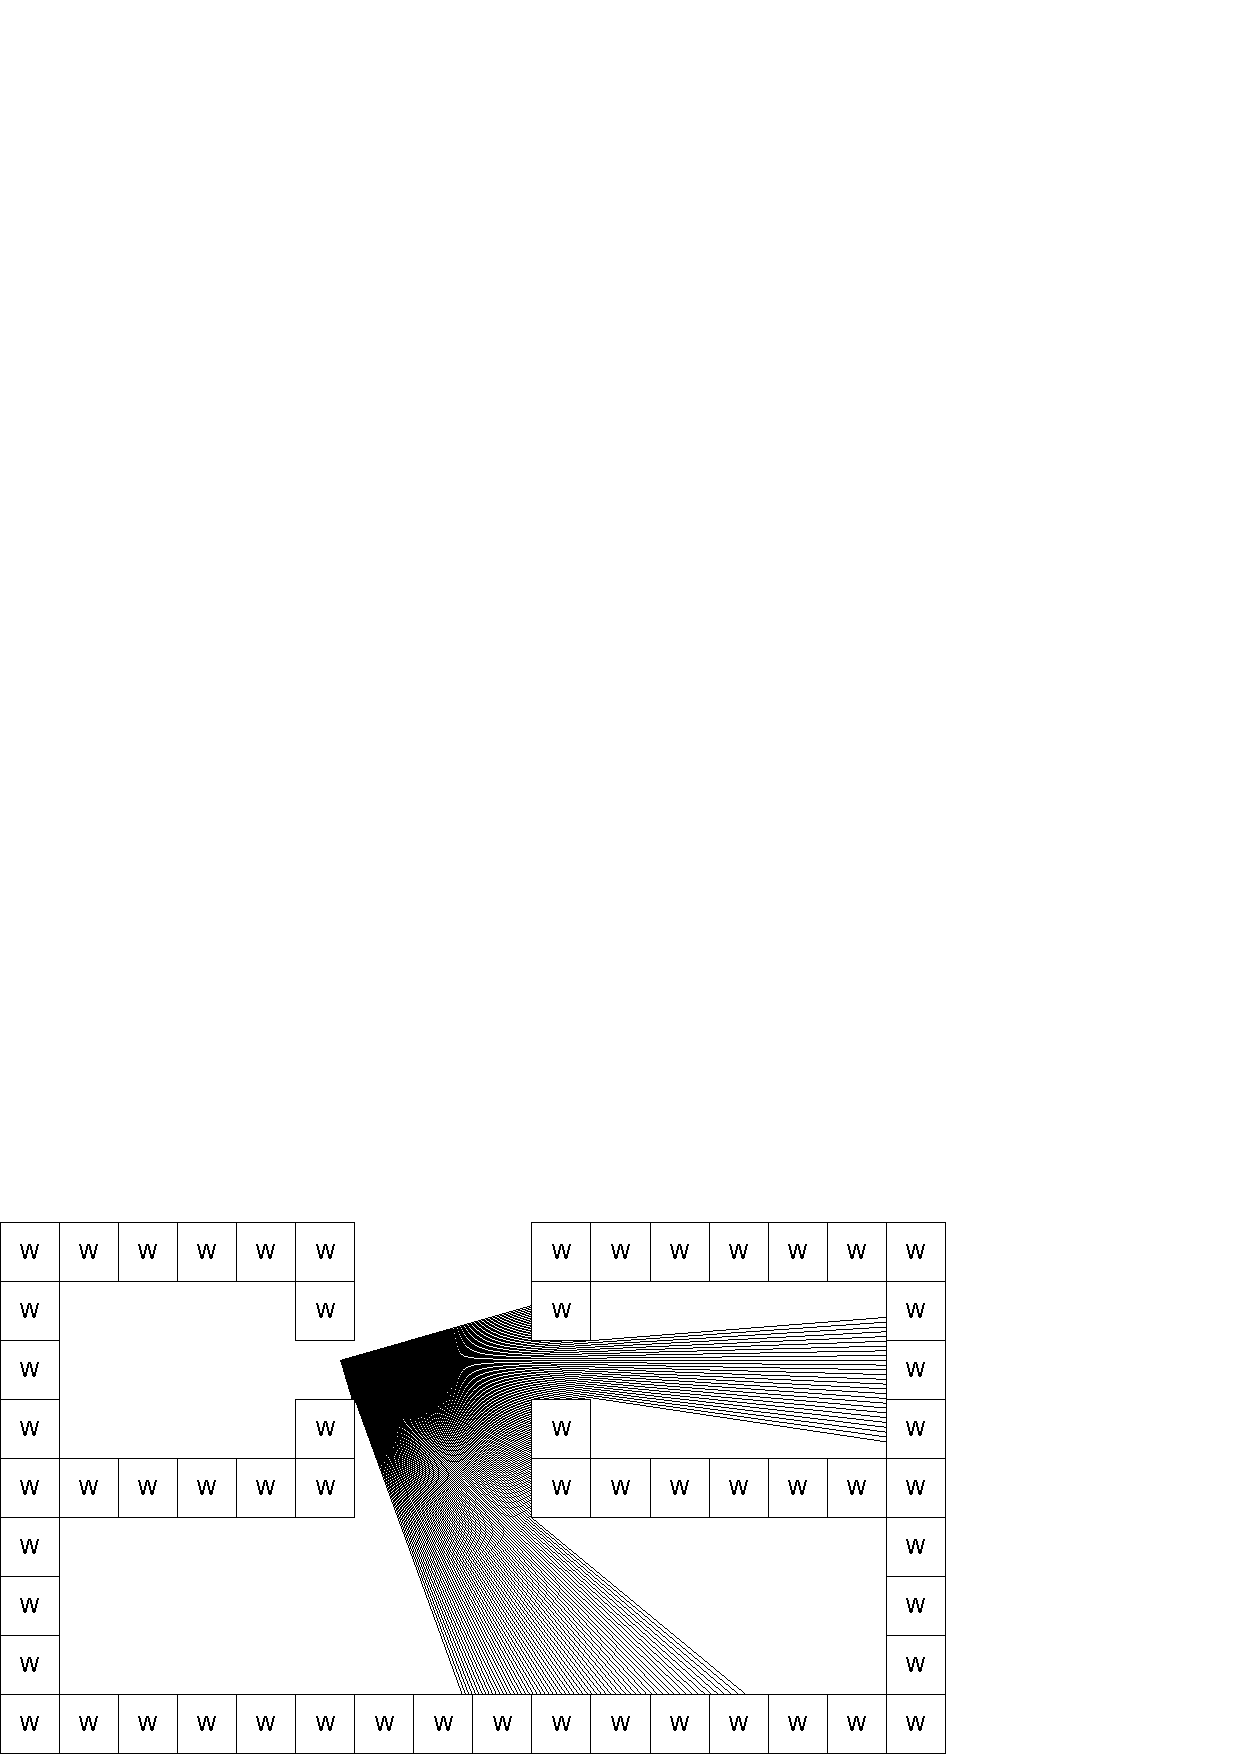
\includegraphics[width=\textwidth]{imgs/drawings/ray_caster_explained/out_room.pdf}
 \caption{Casting 320 rays (one for each column) for a screen of resolution 320x200} \label{fig:Raycasting2}
\end{figure}

\begin{figure}[H]
  \centering
 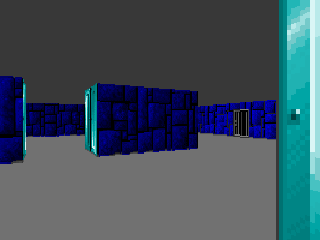
\includegraphics[width=\textwidth]{imgs/drawings/ray_caster_explained/out_door.png}
 \caption{Rendition of the 320 column of pixels (with texturing).} 
\end{figure} 


\subsection{Life of a frame}
As we saw when we unrolled the loop, the action scene is made of frames in a loop which is pseudo code looks as follow:\\
\par
\begin{minipage}{\textwidth}
 \lstinputlisting[language=C]{code/flawded_game_loop.c}
 \end{minipage}
\par
This is a pretty standard loop for an engine from the 90s however this architecture has a major flaw. Each slice of the game has a different duration which makes the game nondeterministic from one machine to an other. Or even between two runs on the same machine. In the next drawing, all three timeslice have different durations:\\
\begin{figure}[H]
\centering
 \includegraphics[width=\textwidth]{imgs/drawings/timer/wrong.pdf}
 
 \end{figure}
  Which explains why it is not possible to record and replay a session. Upon replaying a recorded game the engine would reach point where it is supposed to update the world at a point in time where no inputs are available, resulting in a different world outcome.\\
 \begin{figure}[H]
\centering
 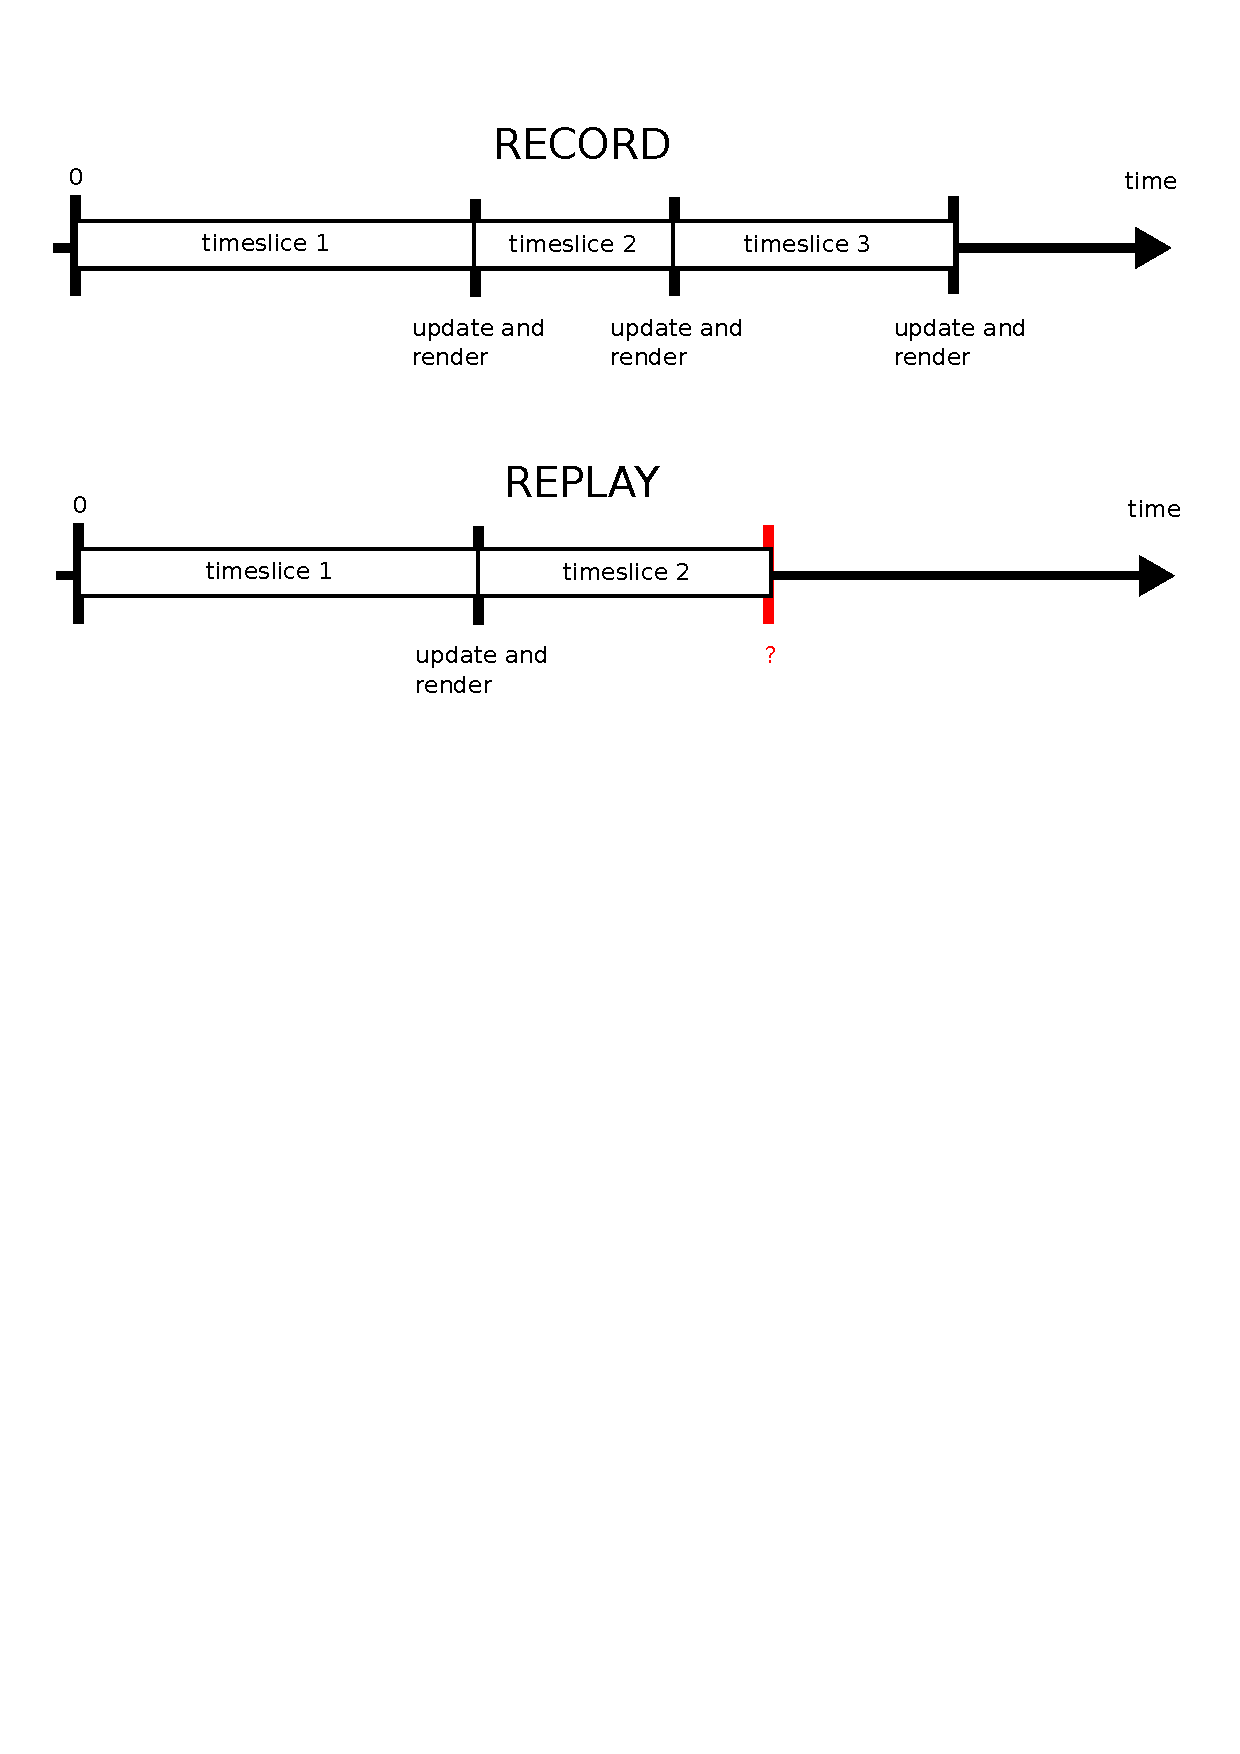
\includegraphics[width=\textwidth]{imgs/drawings/timer/replay.pdf}
 
 \end{figure}
\par
To solve this problem during the demo, the game disregards the timer and simulate things at fixed timesteps.\\
\par
\bu{Trivia :} In 1993, Doom engine would solve this issue by simulating the world at fixed intervals:\\
\par
\begin{minipage}{\textwidth}
 \lstinputlisting[language=C]{code/fixed_game_loop.c}
 \end{minipage}
\par
 \begin{figure}[H]
\centering
 \includegraphics[width=\textwidth]{imgs/drawings/timer/fixed.pdf}
 
 \end{figure}

\subsection{Life of a 3D frame}
Before diving into details, here is an overview of the five stages involved in drawing a 3D scene.\\
\begin{enumerate}
 \item Clear the framebuffer by drawing the floor and the ceiling (both solid color).
 \item For each column of pixel on screen. cast a ray for each column of pixel from the player the wall. Draw a textured column of pixels inversely proportional to the distance.
 \item Draw the things (enemies, lamps, barrels).
 \item Draw the weapon.	
 \item Flip buffers: Instruct CRT Controller to use the framebuffer just composed on next vsync.
\end{enumerate}
During the entire process, all assets come from one file VMSWAP via the Page Manager.\\
\begin{enumerate}
	\item Textures for the wall are stored uncompressed.
	\item Sprites are stored in RAM compressed (via RLE encoding skipping transparent parts). They are decompressed on the fly upon drawing each column of pixels.
\end{enumerate}
As a visual aid here is what the framebuffer looks like after each stage:\\
\begin{figure}[H]
\centering
 \fullimage{wolf3d_1_background.png}
 \caption{Phase 1: Clear screen}
 \end{figure}




\begin{figure}[H]
 \centering
  \fullimage{wolf3d_4_partial_wall_32rays.png}
  \caption{Phase 2: Drawing Walls: 40 rays} 
\end{figure}
\begin{minipage}{.4\textwidth}
 \end{minipage}
\begin{minipage}{.6\textwidth}
\begin{figure}[H]
  \begin{flushright}
 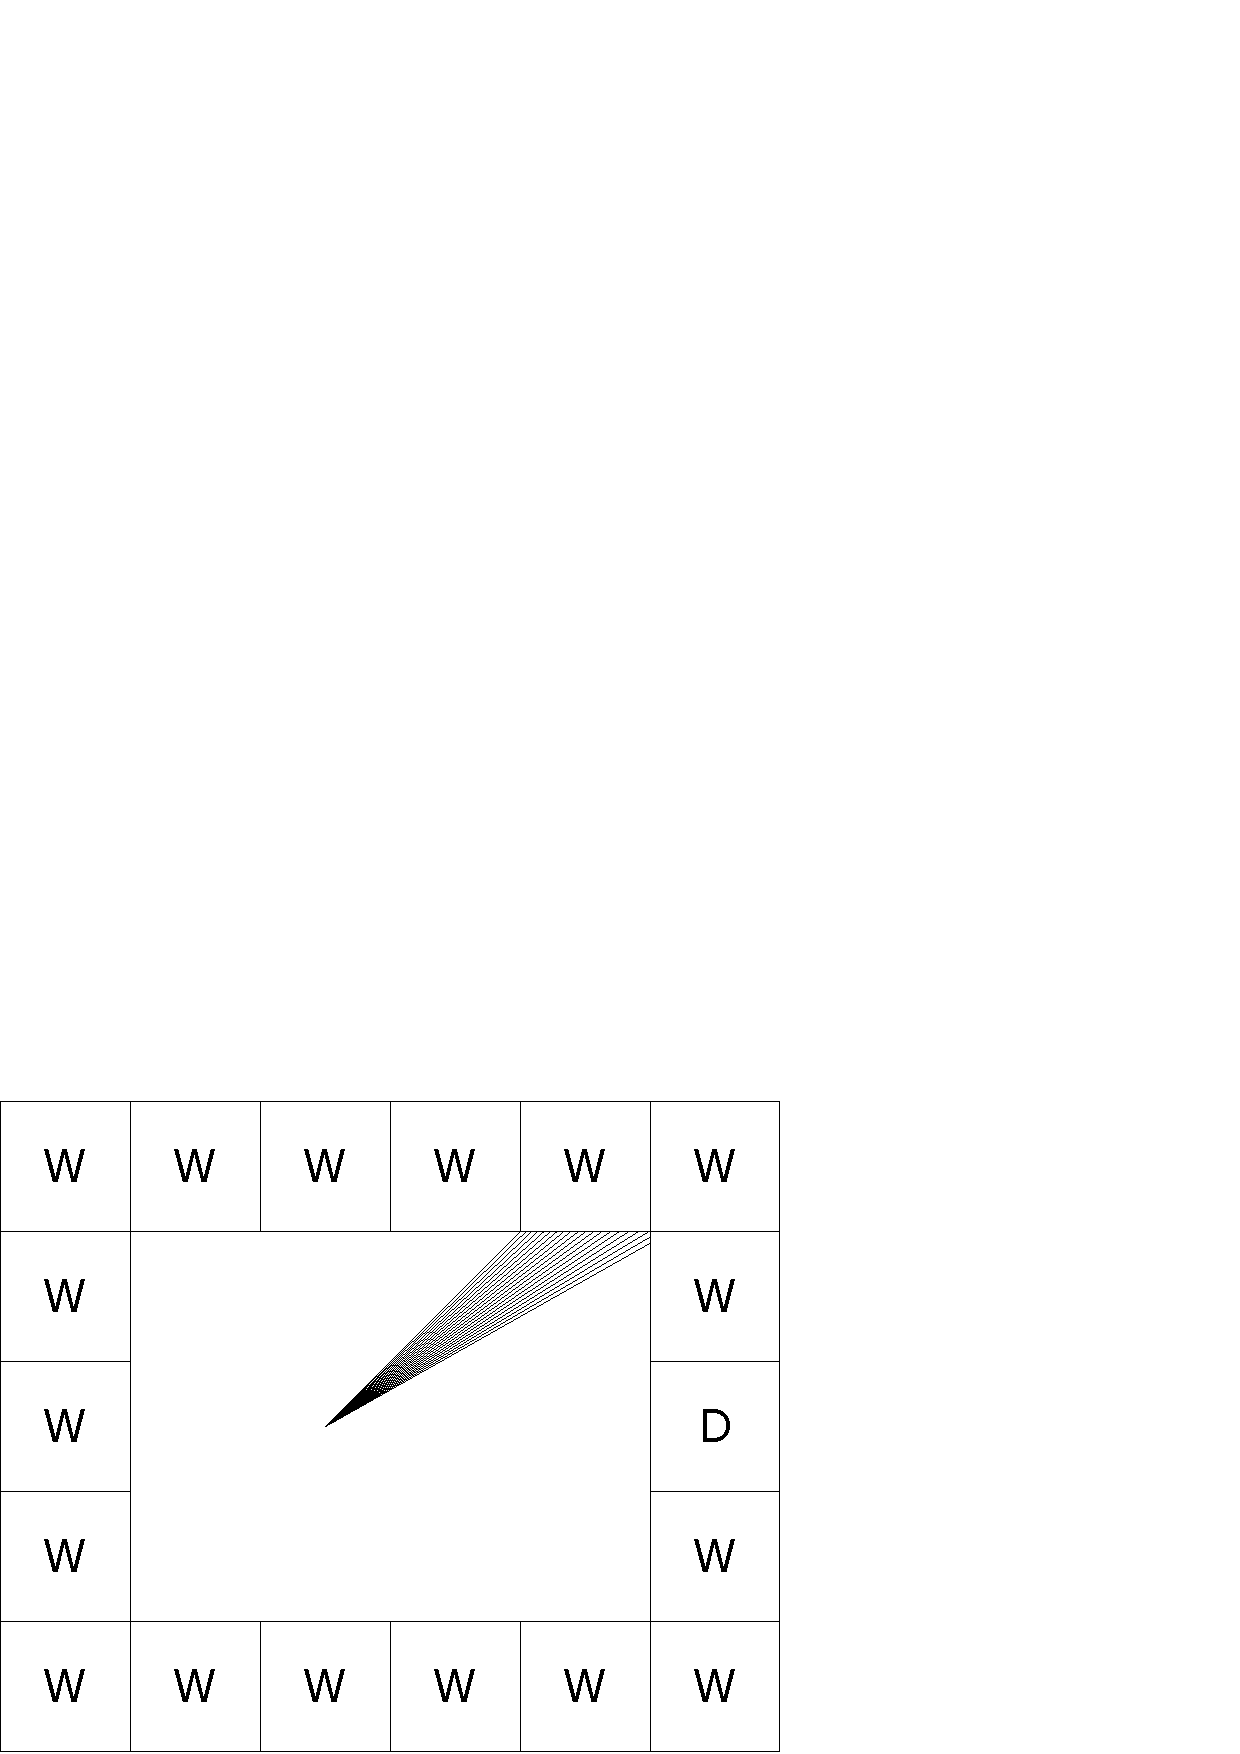
\includegraphics[width=.9\textwidth]{imgs/drawings/ray_caster_explained/beginning10.pdf}
   \end{flushright}
\end{figure}
\end{minipage}




 
\begin{figure}[H]
 \centering
  \fullimage{wolf3d_5_partialwalls_160rays.png}
 \caption{Phase 2: Drawing Walls: 160 rays}  
\end{figure}
 \begin{minipage}{.4\textwidth}
 \end{minipage}
\begin{minipage}{.6\textwidth}
\begin{figure}[H]
  \begin{flushright}
 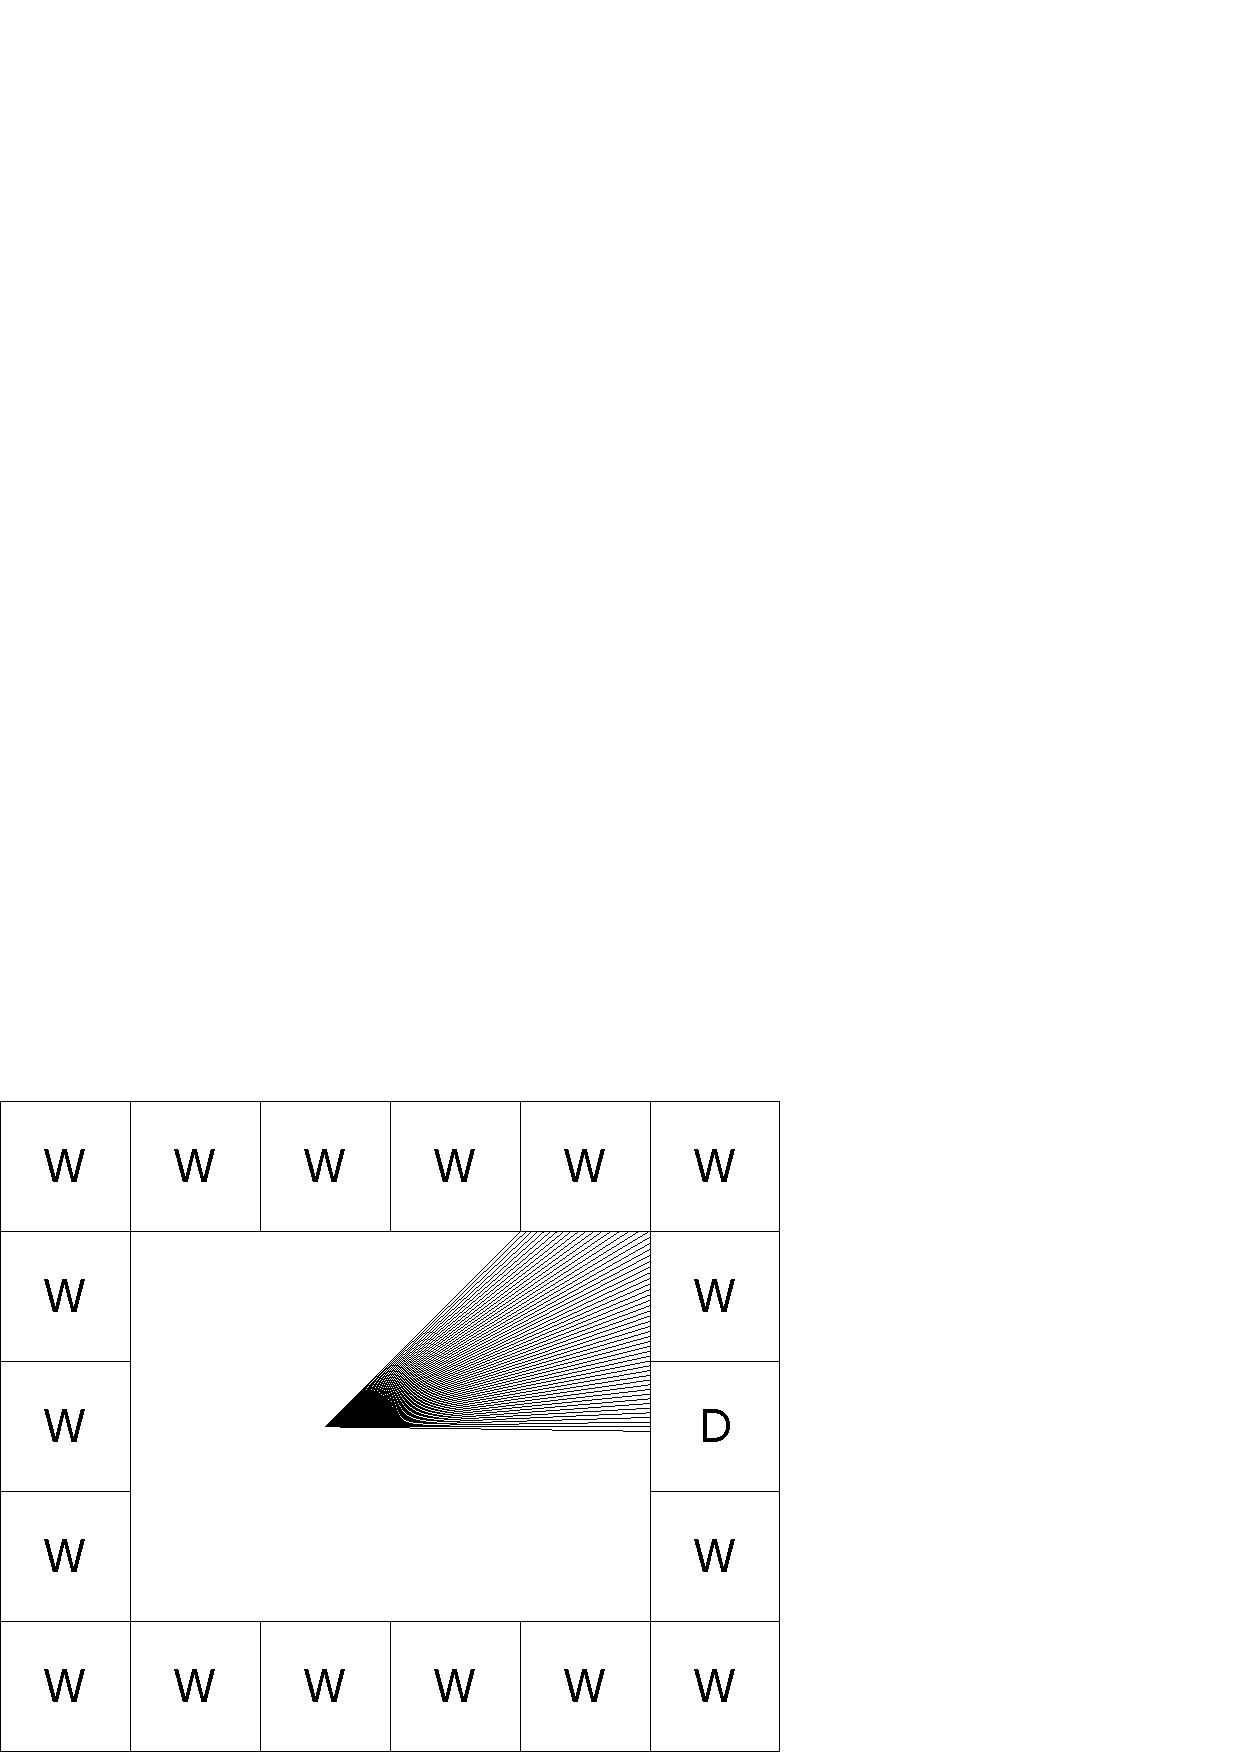
\includegraphics[width=.9\textwidth]{imgs/drawings/ray_caster_explained/beginning50.pdf}
   \end{flushright}
\end{figure}
\end{minipage}



 
 \begin{figure}[H]
\centering
 \fullimage{wolf3d_2_walls.png}
 \caption{Phase 2: Drawing Walls: completed} 
 \end{figure}
\begin{minipage}{.4\textwidth}
 \end{minipage}
\begin{minipage}{.6\textwidth}
\begin{figure}[H]
  \begin{flushright}
 
\includegraphics[width=.9\textwidth]{imgs/drawings/ray_caster_explained/beginning.pdf}
   \end{flushright}
\end{figure}
\end{minipage}




 
 
 \begin{figure}[H]
\centering
 \fullimage{wolf3d_6_scaled}
 \caption{Phase 3: Drawing Things (a.k.a: Scaled, a.k.a: Sprites)} 
 \end{figure}
Note that during this step, clipping is performed.




 \begin{figure}[H]
\centering
 \fullimage{wolf3d_7_fullframe.png}
 \caption{Phase 4: Drawing Weapon} 
 \end{figure}
 













\subsection{3D setup}
Before starting to draw frames, the 3D renderer needs to setup the VRAM with static elements. The 3D view is not fullscreen but it is contained in a HUD\footnote{Head-up display}:
\begin{figure}[H]
  \centering
 \fullimage{hud_empty.png}
\end{figure}
This HUD is drawn only once at the beginning of the 3D phase and it has to be drawn in all three pages. For each new frame, the engine will draw the 3D view in the allocated region. The stats contained in the blue part at the bottom of the screen (Level, Score, Lives, Status, Health, Ammo, Current weapon) get a special treatment via an other VGA trick.\\
\par

The hardware chapter described the Mode 12h which. Despite being unfit for games it still had something interesting. Mode 12h is a 16 colors mode where each four bits are spread across the VGA banks. Since all write operation are one byte, you can see how it would have been difficult to plot a single pixel without changing the other stored in the same bytes. One would have to do four read, four xor and four writes. But the designed of the VGA were not complete sadist they added some circuitry to simplify this operation. For each bank, they added one latche in from of a configurable ALU:\\
\par
 \begin{figure}[H]
\centering
 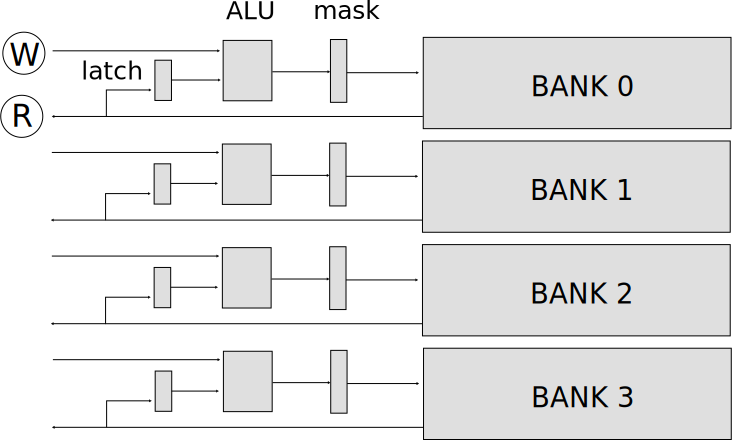
\includegraphics[width=\textwidth]{imgs/drawings/latches.pdf}
 \end{figure}
In this architecture, each time VRAM is read, the latch from the corresponding bank is loaded with the read value. And each time a value is written, it can be composed via the latched value and the ALU. Which allowed mode 12h programmer to plot a point easily:\\
\par
TODO: Insert code sample.\\
\par
Mode Y does not need latches to operate since values are stored in byte and banks can be updated individually thanks to the mask. However hackers\footnote{Michael Abrash Grahic Programming Black Book: Chapter 48 -- Mode X Marks the Latch} found that these latches are still active in  Mode-Y. And by getting a little bit creative and repurposing them, one could copy four pixels from one area of the VRAM to an other with just one read and write to the RAM!\\
\par
To take full advantage of this optimization, the 3D renderer upload images to the VRAM above the third page. Sprites 91 to 134 are latched in VRAM.\\

\begin{minipage}{.23\textwidth}
     \fullimage{latched/91.png}
  \end{minipage}
\begin{minipage}{.23\textwidth}
     \fullimage{latched/92.png}
  \end{minipage}
\begin{minipage}{.23\textwidth}
     \fullimage{latched/93.png}
  \end{minipage}
\begin{minipage}{.23\textwidth}
     \fullimage{latched/94.png}
  \end{minipage}
\par


\begin{minipage}{.095\textwidth}
     \fullimage{latched/99.png}
  \end{minipage}
\begin{minipage}{.095\textwidth}
     \fullimage{latched/100.png}
  \end{minipage}
\begin{minipage}{.095\textwidth}
     \fullimage{latched/101.png}
  \end{minipage}
\begin{minipage}{.095\textwidth}
     \fullimage{latched/102.png}
  \end{minipage}
\begin{minipage}{.095\textwidth}
     \fullimage{latched/103.png}
  \end{minipage}
\begin{minipage}{.095\textwidth}
     \fullimage{latched/104.png}
  \end{minipage}
\begin{minipage}{.095\textwidth}
     \fullimage{latched/105.png}
  \end{minipage}
\begin{minipage}{.095\textwidth}
     \fullimage{latched/106.png}
  \end{minipage}
\begin{minipage}{.095\textwidth}
     \fullimage{latched/107.png}
  \end{minipage}
\begin{minipage}{.095\textwidth}
     \fullimage{latched/108.png}
  \end{minipage}
\par


\begin{minipage}{.3\textwidth}
     \fullimage{latched/109.png}
  \end{minipage}
\begin{minipage}{.3\textwidth}
     \fullimage{latched/110.png}
  \end{minipage}
\begin{minipage}{.3\textwidth}
     \fullimage{latched/111.png}
  \end{minipage}
\par



\begin{minipage}{.3\textwidth}
     \fullimage{latched/112.png}
  \end{minipage}
\begin{minipage}{.3\textwidth}
     \fullimage{latched/113.png}
  \end{minipage}
\begin{minipage}{.3\textwidth}
     \fullimage{latched/114.png}
  \end{minipage}
\par



  \begin{minipage}{.3\textwidth}
     \fullimage{latched/115.png}
  \end{minipage}
\begin{minipage}{.3\textwidth}
     \fullimage{latched/116.png}
  \end{minipage}
\begin{minipage}{.3\textwidth}
     \fullimage{latched/117.png}
  \end{minipage}
\par





  \begin{minipage}{.3\textwidth}
     \fullimage{latched/118.png}
  \end{minipage}
\begin{minipage}{.3\textwidth}
     \fullimage{latched/119.png}
  \end{minipage}
\begin{minipage}{.3\textwidth}
     \fullimage{latched/120.png}
  \end{minipage}
\par



  \begin{minipage}{.3\textwidth}
     \fullimage{latched/121.png}
  \end{minipage}
\begin{minipage}{.3\textwidth}
     \fullimage{latched/122.png}
  \end{minipage}
\begin{minipage}{.3\textwidth}
     \fullimage{latched/123.png}
  \end{minipage}
\par

    \begin{minipage}{.3\textwidth}
     \fullimage{latched/124.png}
  \end{minipage}
\begin{minipage}{.3\textwidth}
     \fullimage{latched/125.png}
  \end{minipage}
\begin{minipage}{.3\textwidth}
     \fullimage{latched/126.png}
  \end{minipage}
\par

    \begin{minipage}{.3\textwidth}
     \fullimage{latched/127.png}
  \end{minipage}
\begin{minipage}{.3\textwidth}
     \fullimage{latched/128.png}
  \end{minipage}
\begin{minipage}{.3\textwidth}
     \fullimage{latched/129.png}
  \end{minipage}
\par

    \begin{minipage}{.3\textwidth}
     \fullimage{latched/130.png}
  \end{minipage}
\begin{minipage}{.3\textwidth}
     \fullimage{latched/131.png}
  \end{minipage}
\begin{minipage}{.3\textwidth}
     \fullimage{latched/132.png}
  \end{minipage}
\par


\begin{minipage}{.1\textwidth}
     \fullimage{latched/95.png}
  \end{minipage}
\begin{minipage}{.1\textwidth}
     \fullimage{latched/96.png}
  \end{minipage}
\begin{minipage}{.1\textwidth}
     \fullimage{latched/97.png}
  \end{minipage}
\begin{minipage}{.1\textwidth}
     \fullimage{latched/98.png}
  \end{minipage}
  \begin{minipage}{.3\textwidth}
     \fullimage{latched/133.png}
  \end{minipage}
\begin{minipage}{.3\textwidth}
     \fullimage{latched/134.png}
  \end{minipage}\
All these assets account for $48*24*4+14*8*16+23*24*32+224*48=34,816$ bytes. There is therefore $2^18-320*208*3 - 34,816=27,648$ bytes unused VRAM in the VGA.\\
\par
Of course, for this trick to work images source and destination have to be aligned on four byte. If you take a look at the location of each elements on screen you can see that elements are aligned on four horizontally. Vertically there is no such issue.
\begin{figure}[H]
  \centering
 \includegraphics[width=\textwidth]{imgs/drawings/hud.pdf}
\end{figure}

While it is faster to write four pixel in two operations, the trick does not provide whic 300\% speed increase since all writes have to be done in all three buffers:\\
\par
\begin{minipage}{\textwidth}
\lstinputlisting[language=C]{code/StatusDrawPic.c}
\end{minipage}



\subsection{Clearing the screen}
At the beginning of a frame, the engine switch to the next buffer and clears the 3D area with ceiling and floor colors. To this effect, it uses the same trick seen in the 2D renderer and sets the VGA bank mask to 15. However since values are written 16 bits at a time, that allows to write 8 pixels at a time:\\ 
\par
\begin{minipage}{\textwidth}
 \lstinputlisting[language=C,morekeywords=asm]{code/VGAClearScreen.c}
 \end{minipage}
\par
As a result, clearing the screen made of 64000 pixels requires only 64000/8 = 8000 write operations. An impressive way to turn an awkward four bank based architecture into a tremendous source of optimizations!\\
\par
Note that the colors are not coming from the maps. They are hardcoded in the engine:\\
\par
\begin{minipage}{\textwidth}
 \lstinputlisting[language=C,morekeywords=byte]{code/vgaCeiling.c}
 \end{minipage}
\par


Following, ceiling colors \cw{0x1D}, \cw{0xBF}, \cw{0x4E} and \cw{0x8D}.\\ 
\par
\scaledimage{.24}{palette_1d.png}
\scaledimage{.24}{palette_bf.png}
\scaledimage{.24}{palette_8d.png}
\scaledimage{.24}{palette_4e.png}






\subsection{Solving the CPU problem}

The hardware chapter describing the CPU capabilities had left the reader with a problem at hands: The machine cannot do floating point operations fast enough. This is a pretty big deal for a 3D engine and all the trigonometry involved. It turns out the solution is to trick the ALU via a technique called "fixed point arithmetic".







\subsubsection{Fixed point}
The normal layout of an \cw{int} is as follow:
\begin{figure}[H]
\centering
 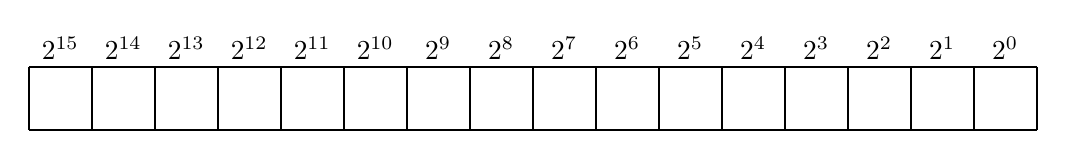
\begin{tikzpicture}[scale=0.8, every node/.style={scale=0.99}]
\draw[thick] (0,0) -- (16,0);
\draw[thick] (0,1) -- (16,1);
\foreach \i in {0,...,16}
{
     \draw[thick] (\i,1) -- (\i,0);
}

\foreach \i in {0,...,15}
{
     \node[] at (15-\i+0.5,1.3){$2^{\i}$}  ;
       
       
     
}
\end{tikzpicture}

 \caption{Integer layout.} \label{fig:int_layout}
 \end{figure}
The value of the sequence of bits \emph{0010010010010010}:
\begin{figure}[H]
\centering
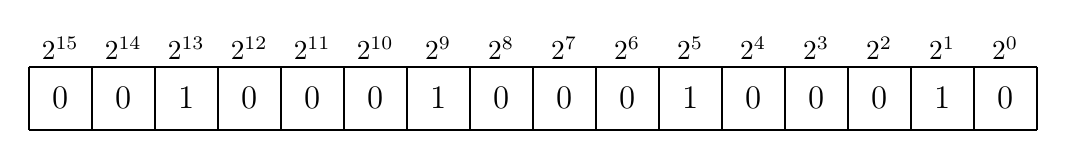
\begin{tikzpicture}[scale=0.8, every node/.style={scale=0.99}]
\draw[thick] (0,0) -- (16,0);
\draw[thick] (0,1) -- (16,1);
\foreach \i in {0,...,16}
{
     \draw[thick] (\i,1) -- (\i,0);
}

\foreach \i in {0,...,15}
{
     \node[] at (15-\i+0.5,1.3){$2^{\i}$}  ;
}

\tikzstyle{fontbf} = [font=\large]
\node[fontbf] at (0.5,0.5){0} ;
\node[fontbf] at (1.5,0.5){0};  
\node[fontbf] at (2.5,0.5){1} ; 
\node[fontbf] at (3.5,0.5){0} ;

\node[fontbf] at (4.5,0.5){0} ;
\node[fontbf] at (5.5,0.5){0};  
\node[fontbf] at (6.5,0.5){1} ; 
\node[fontbf] at (7.5,0.5){0} ;

\node[fontbf] at (8.5,0.5){0} ;
\node[fontbf] at (9.5,0.5){0};  
\node[fontbf] at (10.5,0.5){1} ; 
\node[fontbf] at (11.5,0.5){0} ;

\node[fontbf] at (12.5,0.5){0} ;
\node[fontbf] at (13.5,0.5){0};  
\node[fontbf] at (14.5,0.5){1} ; 
\node[fontbf] at (15.5,0.5){0} ;


\end{tikzpicture}

 \caption{Integer example.} \label{fig:mips}
 \end{figure}

Represents $ 2^{13} + 2^9 + 2^5 + 2^1 =  8738 $.\\
 \par

Fixed Point allows to keep track of fractions while still using the integer operations of the CPU. The machine manipulates what are supposed to be integer numbers but the programmers sees them as a value containing an integer part and a fractional part:\\
\par
\begin{figure}[H]
 \centering
  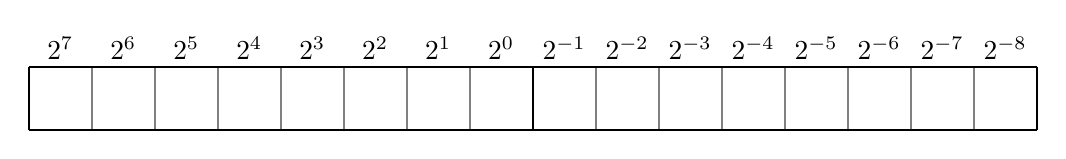
\begin{tikzpicture}[scale=0.8, every node/.style={scale=0.99}]


\colorlet{LighterMark}{black!50}

\foreach \i in {1,...,15}
{
     \draw[thick,LighterMark] (\i,1) -- (\i,0);
}

     \draw[thick,black] (0,1) -- (0,0);
      \draw[thick,black] (8,1) -- (8,0);
      \draw[thick,black] (16,1) -- (16,0);
      
\draw[thick,black] (0,0) -- (16,0);
\draw[thick,black] (0,1) -- (16,1);
 

%\foreach \i[evaluate={\pow=int(7-\i)}] in {0,...,7}
\foreach \i[evaluate={\pow=int(7-\i)}] in {0,...,7}
{
   \node[] at (\i+0.5,1.3){$2^{\pow}$  }  ;
      
         
     
}

%\foreach \i[evaluate={\pow=int((\i-7)*2)}]  in {8,...,15}
\foreach \i[evaluate={\pow=int(\i-7)}]  in {8,...,15}
{
     \node[] at (\i+0.5,1.3){$2^{-\pow}$}  ;
}




\end{tikzpicture}

 \caption{Fixed point layout 8:8 (8-bits for integer part and 8 bits for fractional part).} \label{fig:mips}
\end{figure}

So the same sequence of bits \emph{0010010010010010}:
\begin{figure}[H]
 \centering
   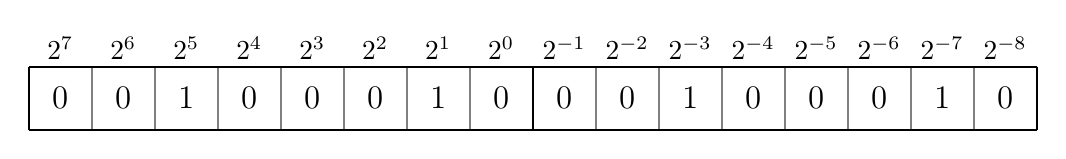
\begin{tikzpicture}[scale=0.8, every node/.style={scale=0.99}]


\colorlet{LighterMark}{black!50}

\foreach \i in {1,...,15}
{
     \draw[thick,LighterMark] (\i,1) -- (\i,0);
}

     \draw[thick,black] (0,1) -- (0,0);
      \draw[thick,black] (8,1) -- (8,0);
      \draw[thick,black] (16,1) -- (16,0);
      
\draw[thick,black] (0,0) -- (16,0);
\draw[thick,black] (0,1) -- (16,1);
 

%\foreach \i[evaluate={\pow=int(7-\i)}] in {0,...,7}
\foreach \i[evaluate={\pow=int(7-\i)}] in {0,...,7}
{
   \node[] at (\i+0.5,1.3){$2^{\pow}$  }  ;
      
         
     
}

%\foreach \i[evaluate={\pow=int((\i-7)*2)}]  in {8,...,15}
\foreach \i[evaluate={\pow=int(\i-7)}]  in {8,...,15}
{
     \node[] at (\i+0.5,1.3){$2^{-\pow}$}  ;
}

\tikzstyle{fontbf} = [font=\large]
\node[fontbf] at (0.5,0.5){0} ;
\node[fontbf] at (1.5,0.5){0};  
\node[fontbf] at (2.5,0.5){1} ; 
\node[fontbf] at (3.5,0.5){0} ;

\node[fontbf] at (4.5,0.5){0} ;
\node[fontbf] at (5.5,0.5){0};  
\node[fontbf] at (6.5,0.5){1} ; 
\node[fontbf] at (7.5,0.5){0} ;

\node[fontbf] at (8.5,0.5){0} ;
\node[fontbf] at (9.5,0.5){0};  
\node[fontbf] at (10.5,0.5){1} ; 
\node[fontbf] at (11.5,0.5){0} ;

\node[fontbf] at (12.5,0.5){0} ;
\node[fontbf] at (13.5,0.5){0};  
\node[fontbf] at (14.5,0.5){1} ; 
\node[fontbf] at (15.5,0.5){0} ;


\end{tikzpicture}

  \caption{Fixed point representation: 8738 is now 34.1328125.} \label{fig:mips}
\end{figure} 

Now represents:\\

$ 2^5 + 2^1 = 34 $ for the integer part.\\
$ 2^{-3}+2^{-7} = 0.1328125 $ for the fractional part.\\
$ = 34.1328125$\\

\bigskip

The beauty of fixed point is that addition and subtraction work exactly like integers from the CPU instruction side:\\




\par
\begin{figure}[H]
 \centering
   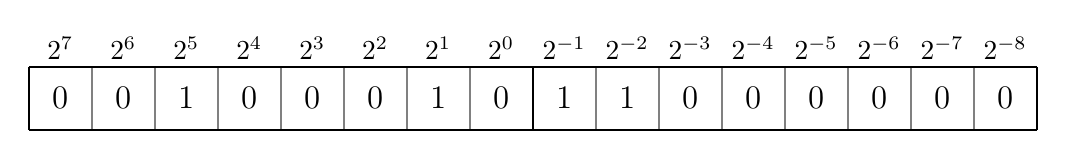
\begin{tikzpicture}[scale=0.8, every node/.style={scale=0.99}]


\colorlet{LighterMark}{black!50}

\foreach \i in {1,...,15}
{
     \draw[thick,LighterMark] (\i,1) -- (\i,0);
}

     \draw[thick,black] (0,1) -- (0,0);
      \draw[thick,black] (8,1) -- (8,0);
      \draw[thick,black] (16,1) -- (16,0);
      
\draw[thick,black] (0,0) -- (16,0);
\draw[thick,black] (0,1) -- (16,1);
 

%\foreach \i[evaluate={\pow=int(7-\i)}] in {0,...,7}
\foreach \i[evaluate={\pow=int(7-\i)}] in {0,...,7}
{
   \node[] at (\i+0.5,1.3){$2^{\pow}$  }  ;
      
         
     
}

%\foreach \i[evaluate={\pow=int((\i-7)*2)}]  in {8,...,15}
\foreach \i[evaluate={\pow=int(\i-7)}]  in {8,...,15}
{
     \node[] at (\i+0.5,1.3){$2^{-\pow}$}  ;
}

\tikzstyle{fontbf} = [font=\large]
\node[fontbf] at (0.5,0.5){0} ;
\node[fontbf] at (1.5,0.5){0};  
\node[fontbf] at (2.5,0.5){1} ; 
\node[fontbf] at (3.5,0.5){0} ;

\node[fontbf] at (4.5,0.5){0} ;
\node[fontbf] at (5.5,0.5){0};  
\node[fontbf] at (6.5,0.5){1} ; 
\node[fontbf] at (7.5,0.5){0} ;

\node[fontbf] at (8.5,0.5){1} ;
\node[fontbf] at (9.5,0.5){1};  
\node[fontbf] at (10.5,0.5){0} ; 
\node[fontbf] at (11.5,0.5){0} ;

\node[fontbf] at (12.5,0.5){0} ;
\node[fontbf] at (13.5,0.5){0};  
\node[fontbf] at (14.5,0.5){0} ; 
\node[fontbf] at (15.5,0.5){0} ;


\end{tikzpicture}


   \caption{34.75} 
\end{figure} 

\begin{figure}[H]
 \centering
   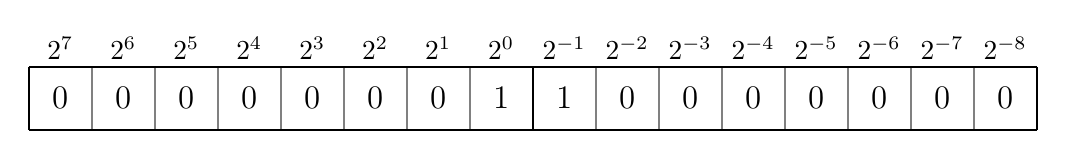
\begin{tikzpicture}[scale=0.8, every node/.style={scale=0.99}]


\colorlet{LighterMark}{black!50}

\foreach \i in {1,...,15}
{
     \draw[thick,LighterMark] (\i,1) -- (\i,0);
}

     \draw[thick,black] (0,1) -- (0,0);
      \draw[thick,black] (8,1) -- (8,0);
      \draw[thick,black] (16,1) -- (16,0);
      
\draw[thick,black] (0,0) -- (16,0);
\draw[thick,black] (0,1) -- (16,1);
 

%\foreach \i[evaluate={\pow=int(7-\i)}] in {0,...,7}
\foreach \i[evaluate={\pow=int(7-\i)}] in {0,...,7}
{
   \node[] at (\i+0.5,1.3){$2^{\pow}$  }  ;
      
         
     
}

%\foreach \i[evaluate={\pow=int((\i-7)*2)}]  in {8,...,15}
\foreach \i[evaluate={\pow=int(\i-7)}]  in {8,...,15}
{
     \node[] at (\i+0.5,1.3){$2^{-\pow}$}  ;
}

\tikzstyle{fontbf} = [font=\large]
\node[fontbf] at (0.5,0.5){0} ;
\node[fontbf] at (1.5,0.5){0};  
\node[fontbf] at (2.5,0.5){0} ; 
\node[fontbf] at (3.5,0.5){0} ;

\node[fontbf] at (4.5,0.5){0} ;
\node[fontbf] at (5.5,0.5){0};  
\node[fontbf] at (6.5,0.5){0} ; 
\node[fontbf] at (7.5,0.5){1} ;

\node[fontbf] at (8.5,0.5){1} ;
\node[fontbf] at (9.5,0.5){0};  
\node[fontbf] at (10.5,0.5){0} ; 
\node[fontbf] at (11.5,0.5){0} ;

\node[fontbf] at (12.5,0.5){0} ;
\node[fontbf] at (13.5,0.5){0};  
\node[fontbf] at (14.5,0.5){0} ; 
\node[fontbf] at (15.5,0.5){0} ;


\end{tikzpicture}

  \caption{+ 1.5} 
\end{figure} 

\begin{figure}[H]
 \centering
   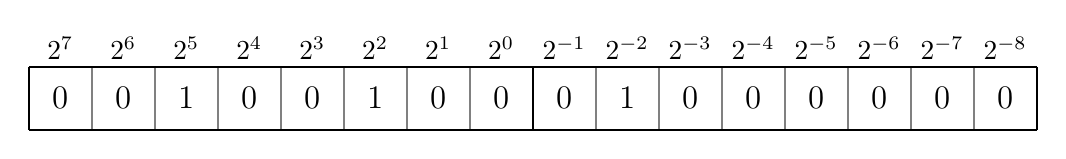
\begin{tikzpicture}[scale=0.8, every node/.style={scale=0.99}]


\colorlet{LighterMark}{black!50}

\foreach \i in {1,...,15}
{
     \draw[thick,LighterMark] (\i,1) -- (\i,0);
}

     \draw[thick,black] (0,1) -- (0,0);
      \draw[thick,black] (8,1) -- (8,0);
      \draw[thick,black] (16,1) -- (16,0);
      
\draw[thick,black] (0,0) -- (16,0);
\draw[thick,black] (0,1) -- (16,1);
 

%\foreach \i[evaluate={\pow=int(7-\i)}] in {0,...,7}
\foreach \i[evaluate={\pow=int(7-\i)}] in {0,...,7}
{
   \node[] at (\i+0.5,1.3){$2^{\pow}$  }  ;
      
         
     
}

%\foreach \i[evaluate={\pow=int((\i-7)*2)}]  in {8,...,15}
\foreach \i[evaluate={\pow=int(\i-7)}]  in {8,...,15}
{
     \node[] at (\i+0.5,1.3){$2^{-\pow}$}  ;
}

\tikzstyle{fontbf} = [font=\large]
\node[fontbf] at (0.5,0.5){0} ;
\node[fontbf] at (1.5,0.5){0};  
\node[fontbf] at (2.5,0.5){1} ; 
\node[fontbf] at (3.5,0.5){0} ;

\node[fontbf] at (4.5,0.5){0} ;
\node[fontbf] at (5.5,0.5){1};  
\node[fontbf] at (6.5,0.5){0} ; 
\node[fontbf] at (7.5,0.5){0} ;

\node[fontbf] at (8.5,0.5){0} ;
\node[fontbf] at (9.5,0.5){1};  
\node[fontbf] at (10.5,0.5){0} ; 
\node[fontbf] at (11.5,0.5){0} ;

\node[fontbf] at (12.5,0.5){0} ;
\node[fontbf] at (13.5,0.5){0};  
\node[fontbf] at (14.5,0.5){0} ; 
\node[fontbf] at (15.5,0.5){0} ;


\end{tikzpicture}

  {\caption{= 36.25}}
\end{figure} 
\par
 Even right shit and left shift trick work:\\
 
 \par
\begin{figure}[H]
 \centering
   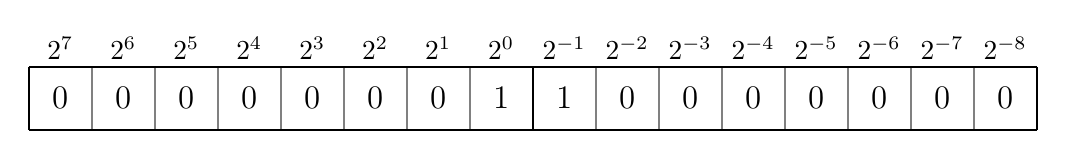
\begin{tikzpicture}[scale=0.8, every node/.style={scale=0.99}]


\colorlet{LighterMark}{black!50}

\foreach \i in {1,...,15}
{
     \draw[thick,LighterMark] (\i,1) -- (\i,0);
}

     \draw[thick,black] (0,1) -- (0,0);
      \draw[thick,black] (8,1) -- (8,0);
      \draw[thick,black] (16,1) -- (16,0);
      
\draw[thick,black] (0,0) -- (16,0);
\draw[thick,black] (0,1) -- (16,1);
 

%\foreach \i[evaluate={\pow=int(7-\i)}] in {0,...,7}
\foreach \i[evaluate={\pow=int(7-\i)}] in {0,...,7}
{
   \node[] at (\i+0.5,1.3){$2^{\pow}$  }  ;
      
         
     
}

%\foreach \i[evaluate={\pow=int((\i-7)*2)}]  in {8,...,15}
\foreach \i[evaluate={\pow=int(\i-7)}]  in {8,...,15}
{
     \node[] at (\i+0.5,1.3){$2^{-\pow}$}  ;
}

\tikzstyle{fontbf} = [font=\large]
\node[fontbf] at (0.5,0.5){0} ;
\node[fontbf] at (1.5,0.5){0};  
\node[fontbf] at (2.5,0.5){0} ; 
\node[fontbf] at (3.5,0.5){0} ;

\node[fontbf] at (4.5,0.5){0} ;
\node[fontbf] at (5.5,0.5){0};  
\node[fontbf] at (6.5,0.5){0} ; 
\node[fontbf] at (7.5,0.5){1} ;

\node[fontbf] at (8.5,0.5){1} ;
\node[fontbf] at (9.5,0.5){0};  
\node[fontbf] at (10.5,0.5){0} ; 
\node[fontbf] at (11.5,0.5){0} ;

\node[fontbf] at (12.5,0.5){0} ;
\node[fontbf] at (13.5,0.5){0};  
\node[fontbf] at (14.5,0.5){0} ; 
\node[fontbf] at (15.5,0.5){0} ;


\end{tikzpicture}

   \caption{1.5} 
\end{figure} 

\par
\begin{figure}[H]
 \centering
   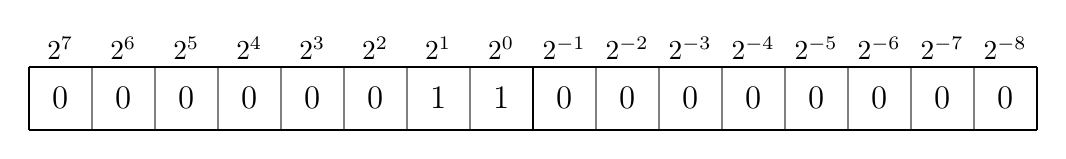
\begin{tikzpicture}[scale=0.8, every node/.style={scale=0.99}]


\colorlet{LighterMark}{black!50}

\foreach \i in {1,...,15}
{
     \draw[thick,LighterMark] (\i,1) -- (\i,0);
}

     \draw[thick,black] (0,1) -- (0,0);
      \draw[thick,black] (8,1) -- (8,0);
      \draw[thick,black] (16,1) -- (16,0);
      
\draw[thick,black] (0,0) -- (16,0);
\draw[thick,black] (0,1) -- (16,1);
 

%\foreach \i[evaluate={\pow=int(7-\i)}] in {0,...,7}
\foreach \i[evaluate={\pow=int(7-\i)}] in {0,...,7}
{
   \node[] at (\i+0.5,1.3){$2^{\pow}$  }  ;
      
         
     
}

%\foreach \i[evaluate={\pow=int((\i-7)*2)}]  in {8,...,15}
\foreach \i[evaluate={\pow=int(\i-7)}]  in {8,...,15}
{
     \node[] at (\i+0.5,1.3){$2^{-\pow}$}  ;
}

\tikzstyle{fontbf} = [font=\large]
\node[fontbf] at (0.5,0.5){0} ;
\node[fontbf] at (1.5,0.5){0};  
\node[fontbf] at (2.5,0.5){0} ; 
\node[fontbf] at (3.5,0.5){0} ;

\node[fontbf] at (4.5,0.5){0} ;
\node[fontbf] at (5.5,0.5){0};  
\node[fontbf] at (6.5,0.5){1} ; 
\node[fontbf] at (7.5,0.5){1} ;

\node[fontbf] at (8.5,0.5){0} ;
\node[fontbf] at (9.5,0.5){0};  
\node[fontbf] at (10.5,0.5){0} ; 
\node[fontbf] at (11.5,0.5){0} ;

\node[fontbf] at (12.5,0.5){0} ;
\node[fontbf] at (13.5,0.5){0};  
\node[fontbf] at (14.5,0.5){0} ; 
\node[fontbf] at (15.5,0.5){0} ;


\end{tikzpicture}

   \caption{1.5 << 2  = 3} 
\end{figure}

\par
\begin{figure}[H]
 \centering
   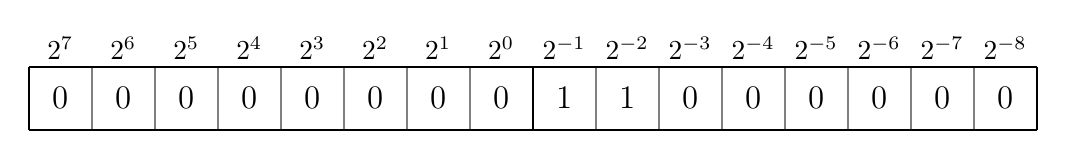
\begin{tikzpicture}[scale=0.8, every node/.style={scale=0.99}]


\colorlet{LighterMark}{black!50}

\foreach \i in {1,...,15}
{
     \draw[thick,LighterMark] (\i,1) -- (\i,0);
}

     \draw[thick,black] (0,1) -- (0,0);
      \draw[thick,black] (8,1) -- (8,0);
      \draw[thick,black] (16,1) -- (16,0);
      
\draw[thick,black] (0,0) -- (16,0);
\draw[thick,black] (0,1) -- (16,1);
 

%\foreach \i[evaluate={\pow=int(7-\i)}] in {0,...,7}
\foreach \i[evaluate={\pow=int(7-\i)}] in {0,...,7}
{
   \node[] at (\i+0.5,1.3){$2^{\pow}$  }  ;
      
         
     
}

%\foreach \i[evaluate={\pow=int((\i-7)*2)}]  in {8,...,15}
\foreach \i[evaluate={\pow=int(\i-7)}]  in {8,...,15}
{
     \node[] at (\i+0.5,1.3){$2^{-\pow}$}  ;
}

\tikzstyle{fontbf} = [font=\large]
\node[fontbf] at (0.5,0.5){0} ;
\node[fontbf] at (1.5,0.5){0};  
\node[fontbf] at (2.5,0.5){0} ; 
\node[fontbf] at (3.5,0.5){0} ;

\node[fontbf] at (4.5,0.5){0} ;
\node[fontbf] at (5.5,0.5){0};  
\node[fontbf] at (6.5,0.5){0} ; 
\node[fontbf] at (7.5,0.5){0} ;

\node[fontbf] at (8.5,0.5){1} ;
\node[fontbf] at (9.5,0.5){1};  
\node[fontbf] at (10.5,0.5){0} ; 
\node[fontbf] at (11.5,0.5){0} ;

\node[fontbf] at (12.5,0.5){0} ;
\node[fontbf] at (13.5,0.5){0};  
\node[fontbf] at (14.5,0.5){0} ; 
\node[fontbf] at (15.5,0.5){0} ;


\end{tikzpicture}

   \caption{1.5 >> 2 = 0.75} 
\end{figure}

The notation for fixed point is \cw{BITS\_FOR\_INTEGER\_PAR:BITS\_FOR\_FRACTIONNAL\_PART}. In the game, player position is \cw{16:16}. The grid location is one shift operation away \cw{player->x >> 16}.


 The special case is when performing multiplication. There are two ways to do it: Either multiply two 32 bits into a 64 bits or drop the precision of both fixed point and multiply then into a 32 bits. Since the 286 and 386 do not have 64 bits registers, wolf does the later (illustrated here with 8:8 for readability):


\par
\begin{figure}[H]
 \centering
   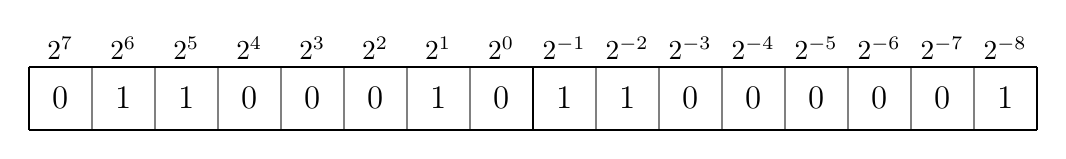
\begin{tikzpicture}[scale=0.8, every node/.style={scale=0.99}]


\colorlet{LighterMark}{black!50}

\foreach \i in {1,...,15}
{
     \draw[thick,LighterMark] (\i,1) -- (\i,0);
}

     \draw[thick,black] (0,1) -- (0,0);
      \draw[thick,black] (8,1) -- (8,0);
      \draw[thick,black] (16,1) -- (16,0);
      
\draw[thick,black] (0,0) -- (16,0);
\draw[thick,black] (0,1) -- (16,1);
 

%\foreach \i[evaluate={\pow=int(7-\i)}] in {0,...,7}
\foreach \i[evaluate={\pow=int(7-\i)}] in {0,...,7}
{
   \node[] at (\i+0.5,1.3){$2^{\pow}$  }  ;
      
         
     
}

%\foreach \i[evaluate={\pow=int((\i-7)*2)}]  in {8,...,15}
\foreach \i[evaluate={\pow=int(\i-7)}]  in {8,...,15}
{
     \node[] at (\i+0.5,1.3){$2^{-\pow}$}  ;
}

\tikzstyle{fontbf} = [font=\large]
\node[fontbf] at (0.5,0.5){0} ;
\node[fontbf] at (1.5,0.5){1};  
\node[fontbf] at (2.5,0.5){1} ; 
\node[fontbf] at (3.5,0.5){0} ;

\node[fontbf] at (4.5,0.5){0} ;
\node[fontbf] at (5.5,0.5){0};  
\node[fontbf] at (6.5,0.5){1} ; 
\node[fontbf] at (7.5,0.5){0} ;

\node[fontbf] at (8.5,0.5){1} ;
\node[fontbf] at (9.5,0.5){1};  
\node[fontbf] at (10.5,0.5){0} ; 
\node[fontbf] at (11.5,0.5){0} ;

\node[fontbf] at (12.5,0.5){0} ;
\node[fontbf] at (13.5,0.5){0};  
\node[fontbf] at (14.5,0.5){0} ; 
\node[fontbf] at (15.5,0.5){1} ;


\end{tikzpicture}

   \caption{98.7539} 
\end{figure} 
\par
\begin{figure}[H]
 \centering
   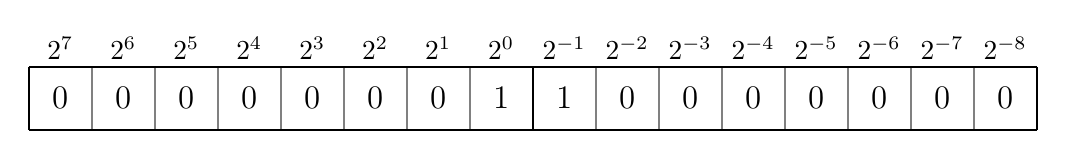
\begin{tikzpicture}[scale=0.8, every node/.style={scale=0.99}]


\colorlet{LighterMark}{black!50}

\foreach \i in {1,...,15}
{
     \draw[thick,LighterMark] (\i,1) -- (\i,0);
}

     \draw[thick,black] (0,1) -- (0,0);
      \draw[thick,black] (8,1) -- (8,0);
      \draw[thick,black] (16,1) -- (16,0);
      
\draw[thick,black] (0,0) -- (16,0);
\draw[thick,black] (0,1) -- (16,1);
 

%\foreach \i[evaluate={\pow=int(7-\i)}] in {0,...,7}
\foreach \i[evaluate={\pow=int(7-\i)}] in {0,...,7}
{
   \node[] at (\i+0.5,1.3){$2^{\pow}$  }  ;
      
         
     
}

%\foreach \i[evaluate={\pow=int((\i-7)*2)}]  in {8,...,15}
\foreach \i[evaluate={\pow=int(\i-7)}]  in {8,...,15}
{
     \node[] at (\i+0.5,1.3){$2^{-\pow}$}  ;
}

\tikzstyle{fontbf} = [font=\large]
\node[fontbf] at (0.5,0.5){0} ;
\node[fontbf] at (1.5,0.5){0};  
\node[fontbf] at (2.5,0.5){0} ; 
\node[fontbf] at (3.5,0.5){0} ;

\node[fontbf] at (4.5,0.5){0} ;
\node[fontbf] at (5.5,0.5){0};  
\node[fontbf] at (6.5,0.5){0} ; 
\node[fontbf] at (7.5,0.5){1} ;

\node[fontbf] at (8.5,0.5){1} ;
\node[fontbf] at (9.5,0.5){0};  
\node[fontbf] at (10.5,0.5){0} ; 
\node[fontbf] at (11.5,0.5){0} ;

\node[fontbf] at (12.5,0.5){0} ;
\node[fontbf] at (13.5,0.5){0};  
\node[fontbf] at (14.5,0.5){0} ; 
\node[fontbf] at (15.5,0.5){0} ;


\end{tikzpicture}

   \caption{* 1.5} 
\end{figure} 
\par
First right shift both operators:\\
\par
\begin{figure}[H]
 \centering
   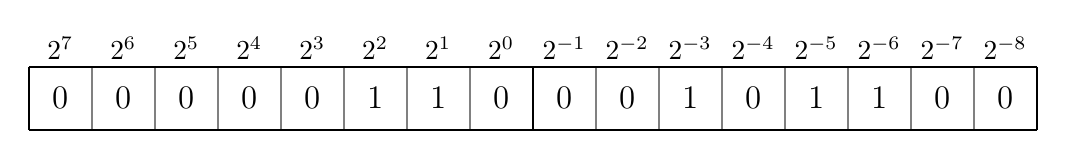
\begin{tikzpicture}[scale=0.8, every node/.style={scale=0.99}]


\colorlet{LighterMark}{black!50}

\foreach \i in {1,...,15}
{
     \draw[thick,LighterMark] (\i,1) -- (\i,0);
}

     \draw[thick,black] (0,1) -- (0,0);
      \draw[thick,black] (8,1) -- (8,0);
      \draw[thick,black] (16,1) -- (16,0);
      
\draw[thick,black] (0,0) -- (16,0);
\draw[thick,black] (0,1) -- (16,1);
 

%\foreach \i[evaluate={\pow=int(7-\i)}] in {0,...,7}
\foreach \i[evaluate={\pow=int(7-\i)}] in {0,...,7}
{
   \node[] at (\i+0.5,1.3){$2^{\pow}$  }  ;
      
         
     
}

%\foreach \i[evaluate={\pow=int((\i-7)*2)}]  in {8,...,15}
\foreach \i[evaluate={\pow=int(\i-7)}]  in {8,...,15}
{
     \node[] at (\i+0.5,1.3){$2^{-\pow}$}  ;
}

\tikzstyle{fontbf} = [font=\large]
\node[fontbf] at (0.5,0.5){0} ;
\node[fontbf] at (1.5,0.5){0};  
\node[fontbf] at (2.5,0.5){0} ; 
\node[fontbf] at (3.5,0.5){0} ;

\node[fontbf] at (4.5,0.5){0} ;
\node[fontbf] at (5.5,0.5){1};  
\node[fontbf] at (6.5,0.5){1} ; 
\node[fontbf] at (7.5,0.5){0} ;

\node[fontbf] at (8.5,0.5){0} ;
\node[fontbf] at (9.5,0.5){0};  
\node[fontbf] at (10.5,0.5){1} ; 
\node[fontbf] at (11.5,0.5){0} ;

\node[fontbf] at (12.5,0.5){1} ;
\node[fontbf] at (13.5,0.5){1};  
\node[fontbf] at (14.5,0.5){0} ; 
\node[fontbf] at (15.5,0.5){0} ;


\end{tikzpicture}

\end{figure} 
\par
\begin{figure}[H]
 \centering
   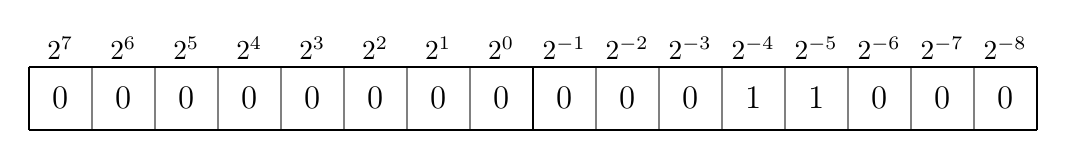
\begin{tikzpicture}[scale=0.8, every node/.style={scale=0.99}]


\colorlet{LighterMark}{black!50}

\foreach \i in {1,...,15}
{
     \draw[thick,LighterMark] (\i,1) -- (\i,0);
}

     \draw[thick,black] (0,1) -- (0,0);
      \draw[thick,black] (8,1) -- (8,0);
      \draw[thick,black] (16,1) -- (16,0);
      
\draw[thick,black] (0,0) -- (16,0);
\draw[thick,black] (0,1) -- (16,1);
 

%\foreach \i[evaluate={\pow=int(7-\i)}] in {0,...,7}
\foreach \i[evaluate={\pow=int(7-\i)}] in {0,...,7}
{
   \node[] at (\i+0.5,1.3){$2^{\pow}$  }  ;
      
         
     
}

%\foreach \i[evaluate={\pow=int((\i-7)*2)}]  in {8,...,15}
\foreach \i[evaluate={\pow=int(\i-7)}]  in {8,...,15}
{
     \node[] at (\i+0.5,1.3){$2^{-\pow}$}  ;
}

\tikzstyle{fontbf} = [font=\large]
\node[fontbf] at (0.5,0.5){0} ;
\node[fontbf] at (1.5,0.5){0};  
\node[fontbf] at (2.5,0.5){0} ; 
\node[fontbf] at (3.5,0.5){0} ;

\node[fontbf] at (4.5,0.5){0} ;
\node[fontbf] at (5.5,0.5){0};  
\node[fontbf] at (6.5,0.5){0} ; 
\node[fontbf] at (7.5,0.5){0} ;

\node[fontbf] at (8.5,0.5){0} ;
\node[fontbf] at (9.5,0.5){0};  
\node[fontbf] at (10.5,0.5){0} ; 
\node[fontbf] at (11.5,0.5){1} ;

\node[fontbf] at (12.5,0.5){1} ;
\node[fontbf] at (13.5,0.5){0};  
\node[fontbf] at (14.5,0.5){0} ; 
\node[fontbf] at (15.5,0.5){0} ;


\end{tikzpicture}

\end{figure} 
\par

Finally multiply them together:

\begin{figure}[H]
 \centering
   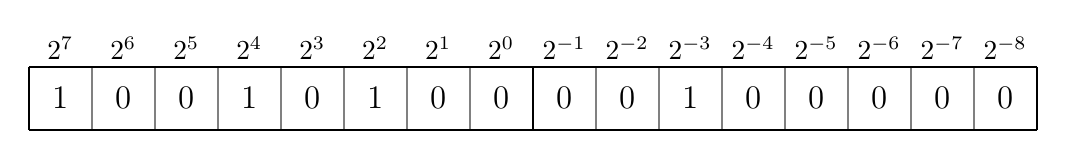
\begin{tikzpicture}[scale=0.8, every node/.style={scale=0.99}]


\colorlet{LighterMark}{black!50}

\foreach \i in {1,...,15}
{
     \draw[thick,LighterMark] (\i,1) -- (\i,0);
}

     \draw[thick,black] (0,1) -- (0,0);
      \draw[thick,black] (8,1) -- (8,0);
      \draw[thick,black] (16,1) -- (16,0);
      
\draw[thick,black] (0,0) -- (16,0);
\draw[thick,black] (0,1) -- (16,1);
 

%\foreach \i[evaluate={\pow=int(7-\i)}] in {0,...,7}
\foreach \i[evaluate={\pow=int(7-\i)}] in {0,...,7}
{
   \node[] at (\i+0.5,1.3){$2^{\pow}$  }  ;
      
         
     
}

%\foreach \i[evaluate={\pow=int((\i-7)*2)}]  in {8,...,15}
\foreach \i[evaluate={\pow=int(\i-7)}]  in {8,...,15}
{
     \node[] at (\i+0.5,1.3){$2^{-\pow}$}  ;
}

\tikzstyle{fontbf} = [font=\large]
\node[fontbf] at (0.5,0.5){1} ;
\node[fontbf] at (1.5,0.5){0};  
\node[fontbf] at (2.5,0.5){0} ; 
\node[fontbf] at (3.5,0.5){1} ;

\node[fontbf] at (4.5,0.5){0} ;
\node[fontbf] at (5.5,0.5){1};  
\node[fontbf] at (6.5,0.5){0} ; 
\node[fontbf] at (7.5,0.5){0} ;

\node[fontbf] at (8.5,0.5){0} ;
\node[fontbf] at (9.5,0.5){0};  
\node[fontbf] at (10.5,0.5){1} ; 
\node[fontbf] at (11.5,0.5){0} ;

\node[fontbf] at (12.5,0.5){0} ;
\node[fontbf] at (13.5,0.5){0};  
\node[fontbf] at (14.5,0.5){0} ; 
\node[fontbf] at (15.5,0.5){0} ;


\end{tikzpicture}

   \caption{148.125} 
\end{figure} 
$128 + 16 + 4 + 0.125 = 148.125 $


Notice that you have to be careful: In the previous example some precision was lost ($ 2^{-8}$) bit disappeared during the $\gg 4$ operation) and an overflow could have occurred (multiplying by 3 would have gone past the precision of 8:8). But with this system, fractions are possible and fast enough!\\
\par
\begin{minipage}{\textwidth}
 \lstinputlisting[language=C]{code/fixed_mul.c}
 \end{minipage}
\par
 \textbf{\underline{Trivia :}}  Fixed Point Arithmetic usage was not limited to PC gaming. Many game console manufactured in the 90s and later had no hardware floating point unit: Sony's original PlayStation (1994) and Sega's Saturn (1994) are examples among many with a design choice that not only reduced the production cost but also maximized the CPU pipeline throughput.
 

 
 


\subsubsection{Coordinate System}
With the CPU/\cw{float}/\cw{int} problem out of the way, it is almost time to study how a ray is cast. A quick reminder on the coordinate system used:
\begin{figure}[H]
  \centering
 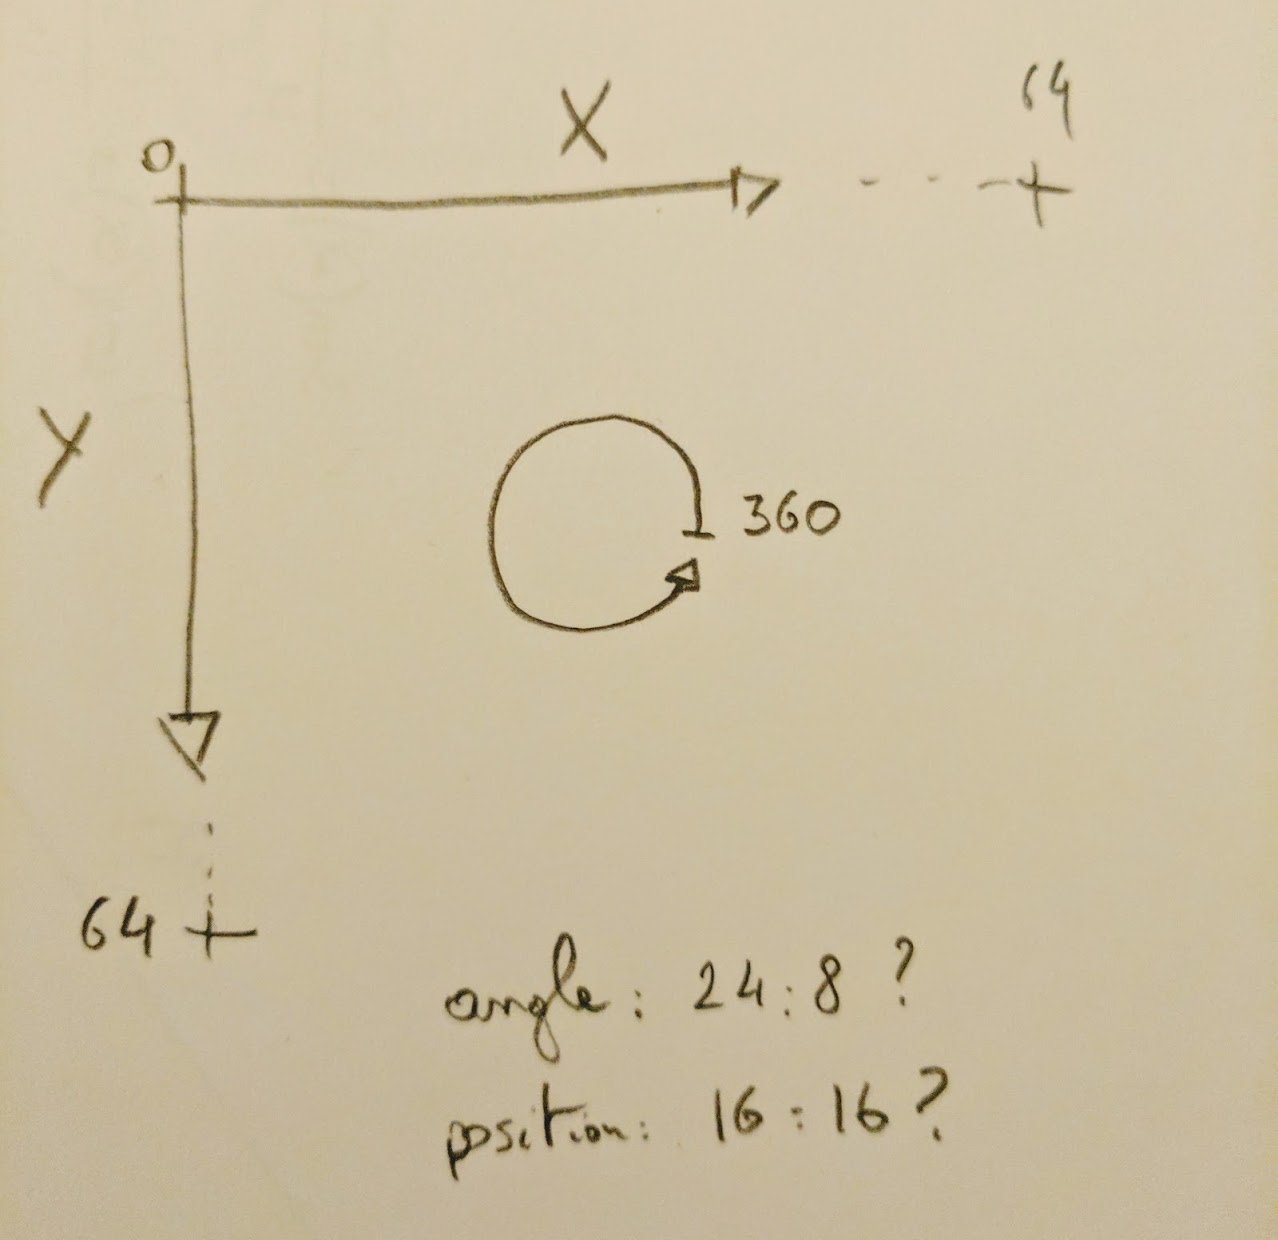
\includegraphics[width=\textwidth]{imgs/drawings/coordinate_system.png}
\end{figure}
\par
A map is 64 by 64. Since one block is 8 feet, maps can be 512 feet wide and tall. Fixed point variables are used all over the place: column height are 24:8. Position is also 24:8. Angle however is an int representing 10th of degrees with range [0, 3600].

















\subsubsection{Square World and RayCasting}
Drawing the walls is all about determining what is visible, what is not and what is in front of what. Michael Abrash's view on the topic tells it all:\\
\par
\begin{fancyquotes}
I want to talk about what is, in my book, the toughest 3-D problem of all, visible surface determination (drawing the proper surface at each pixel), and its close relative, culling (discarding non-visible polygons as quickly as possible, a way of accelerating visible surface determination). In the interests of brevity, I’ll use the abbreviation VSD to mean both visible surface determination and culling from now on.
 \bigskip \\
Why do I think VSD is the toughest 3-D challenge? Although rasterization issues such as texture mapping are fascinating and important, they are tasks of relatively finite scope, and are being moved into hardware as 3-D accelerators appear; also, they only scale with increases in screen resolution, which are relatively modest.
 \bigskip \\
In contrast, VSD is an open-ended problem, and there are dozens of approaches currently in use. Even more significantly, the performance of VSD, done in an unsophisticated fashion, scales directly with scene complexity, which tends to increase as a square or cube function, so this very rapidly becomes the limiting factor in doing realistic worlds. I expect VSD increasingly to be the dominant issue in realtime PC 3-D over the next few years, as 3-D worlds become increasingly detailed.
 \bigskip \\
\textbf{Michael Abrash - Programmer}
 \end{fancyquotes}
 \par
VSD is not only complicated to get right, it is also expensive to perform. It is easy to understand with a small example where objects are of free form with no alignment.

\par
\begin{figure}[H]
\centering
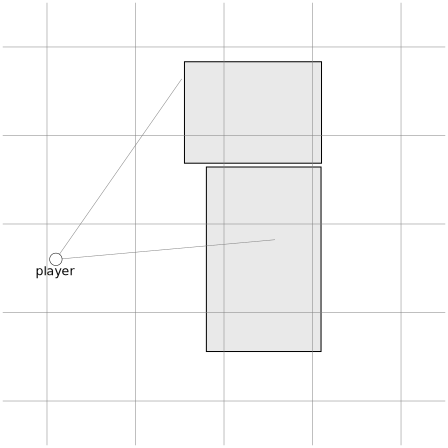
\includegraphics[width=\textwidth]{imgs/drawings/casting_a_ray/situation.pdf}
 %\documentclass[tikz,border=2pt,png]{standalone}
\usepackage{tkz-euclide}
\usetkzobj{all}
\begin{document}
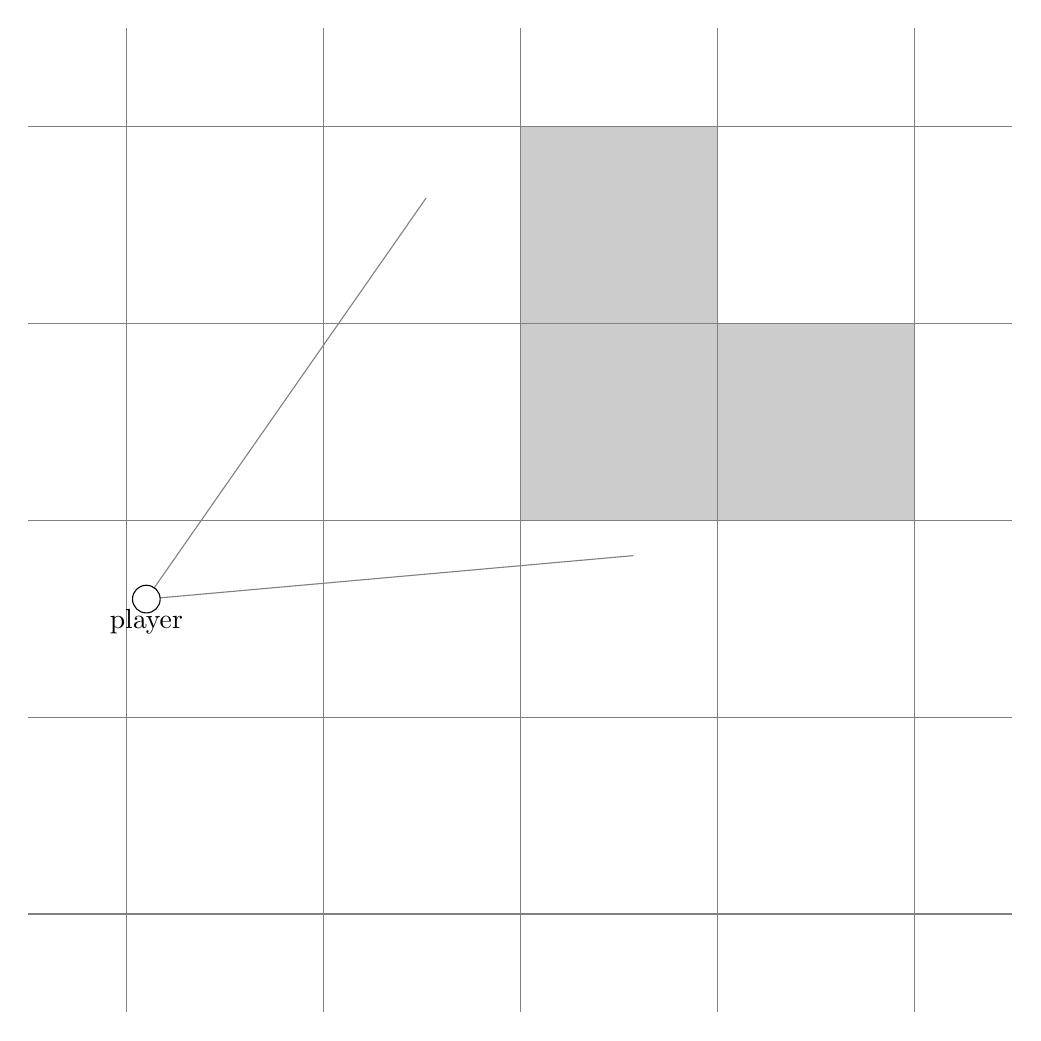
\begin{tikzpicture}[scale=2.5]


\coordinate(player) at (2.1,3.6) {};
\coordinate(intercept) at (4,5.2) {};






\fill[black!20!white, draw=black] (4,5) rectangle (5,6);
\fill[black!20!white, draw=black] (4,4) rectangle (5,5);
\fill[black!20!white, draw=black] (5,4) rectangle (6,5);

%grid
% vertical lines
\draw[draw=gray] (2,1.5) -- (2,6.5) ;
\draw[draw=gray] (3,1.5) -- (3,6.5) ;
\draw[draw=gray] (4,1.5) -- (4,6.5) ;
\draw[draw=gray] (5,1.5) -- (5,6.5) ;
\draw[draw=gray] (6,1.5) -- (6,6.5) ;

% horizontal lines
\draw[draw=gray] (1.5,2) -- (6.5,2) ;
\draw[draw=gray] (1.5,3) -- (6.5,3) ;
\draw[draw=gray] (1.5,4) -- (6.5,4) ;
\draw[draw=gray] (1.5,5) -- (6.5,5) ;
\draw[draw=gray] (1.5,6) -- (6.5,6) ;
%\draw[] 



\draw(player)node[below]{player};


\coordinate[](left_edge) at ($(player)!1!15:(intercept)$);
\coordinate[](right_edge) at ($(player)!1!325:(intercept)$);
\draw[draw=gray] (player) -> (left_edge) ;
\draw[draw=gray] (player) -> (right_edge) ;
\fill[draw=black, fill=white] (player) circle (2pt);



\end{tikzpicture}
\end{document}

\end{figure}


A possible approach to find wall intersection would be to do ray marching which consist in checking at regular interval. But that would be very CPU intensive and even with fixed point that would not be fast enough.
\begin{figure}[H]
\centering
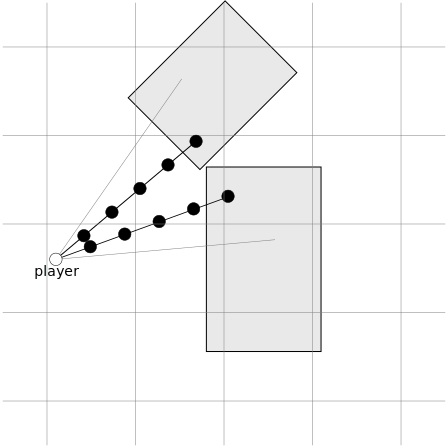
\includegraphics[width=\textwidth]{imgs/drawings/casting_a_ray/unaligned.pdf}
 %\documentclass[tikz,border=2pt,png]{standalone}
\usepackage{tkz-euclide}
\begin{document}
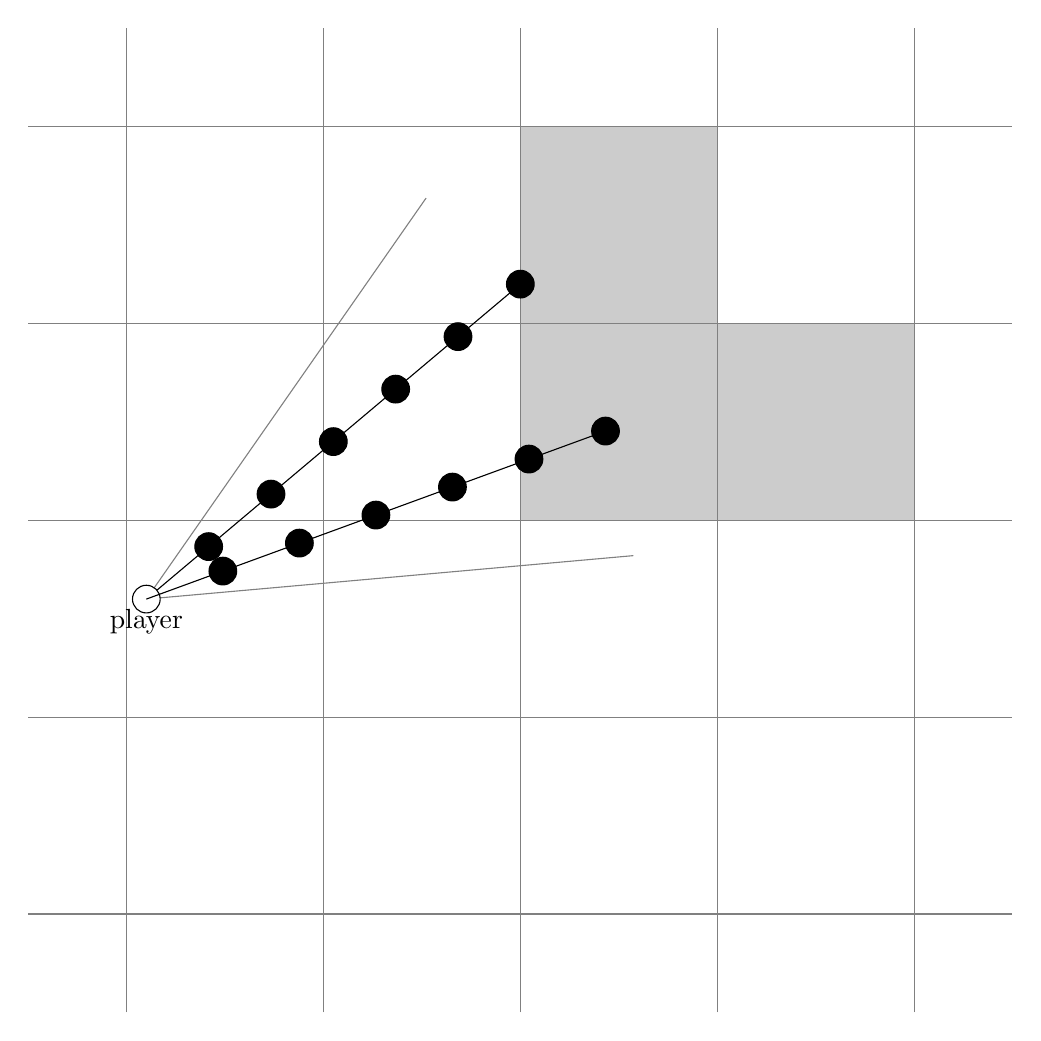
\begin{tikzpicture}[scale=2.5]


\coordinate(player) at (2.1,3.6) {};
\coordinate(intercept) at (4,5.2) {};

%FOV
\coordinate[](left_edge) at ($(player)!1!15:(intercept)$);
\coordinate[](right_edge) at ($(player)!1!325:(intercept)$);
\draw[draw=gray] (player) -> (left_edge) ;
\draw[draw=gray] (player) -> (right_edge) ;




\fill[black!20!white, draw=black] (4,5) rectangle (5,6);
\fill[black!20!white, draw=black] (4,4) rectangle (5,5);
\fill[black!20!white, draw=black] (5,4) rectangle (6,5);

%grid
% vertical lines
\draw[draw=gray] (2,1.5) -- (2,6.5) ;
\draw[draw=gray] (3,1.5) -- (3,6.5) ;
\draw[draw=gray] (4,1.5) -- (4,6.5) ;
\draw[draw=gray] (5,1.5) -- (5,6.5) ;
\draw[draw=gray] (6,1.5) -- (6,6.5) ;

% horizontal lines
\draw[draw=gray] (1.5,2) -- (6.5,2) ;
\draw[draw=gray] (1.5,3) -- (6.5,3) ;
\draw[draw=gray] (1.5,4) -- (6.5,4) ;
\draw[draw=gray] (1.5,5) -- (6.5,5) ;
\draw[draw=gray] (1.5,6) -- (6.5,6) ;
%\draw[] 

\draw[draw=black] (player) -- (intercept) ;
\fill[draw=black, fill=white] (player) circle (2pt);
\fill[draw=black] (intercept) circle (2pt);

\draw(player)node[below]{player};



\fill[draw=black] ( $ (player)!5/6!(intercept) $ ) circle (2pt);
\fill[draw=black] ( $ (player)!4/6!(intercept) $ ) circle (2pt);
\fill[draw=black] ( $ (player)!3/6!(intercept) $ ) circle (2pt);
\fill[draw=black] ( $ (player)!2/6!(intercept) $ ) circle (2pt);
\fill[draw=black] ( $ (player)!1/6!(intercept) $ ) circle (2pt);


\coordinate[](missed_intercept) at ($(player)!1!340:(intercept)$);
\draw[draw=black] (player) -- (missed_intercept) ;
\fill[draw=black] (missed_intercept) circle (2pt);
\fill[draw=black] ( $ (player)!5/6!(missed_intercept) $ ) circle (2pt);
\fill[draw=black] ( $ (player)!4/6!(missed_intercept) $ ) circle (2pt);
\fill[draw=black] ( $ (player)!3/6!(missed_intercept) $ ) circle (2pt);
\fill[draw=black] ( $ (player)!2/6!(missed_intercept) $ ) circle (2pt);
\fill[draw=black] ( $ (player)!1/6!(missed_intercept) $ ) circle (2pt);

\end{tikzpicture}
\end{document}

\end{figure}


However by adding some contraint to the world the problem can becomes much simpler. If the world is made of square block alixed with axis and evenly distributed on a grid, the solution giving 100\% accuracy and low runtime is to check for 'hit` each time a ray cross the grid. This is the choice Wolfenstein 3D made and that explains why it can only draw perpendicular walls, all of them being 8 feet by 8 feet by 8 feet cubes.
\begin{figure}[H]
\centering
\includegraphics[width=\textwidth]{imgs/drawings/casting_a_ray/fixed.pdf}
 %\documentclass[tikz,border=2pt,png]{standalone}
\usepackage{tkz-euclide}
\begin{document}
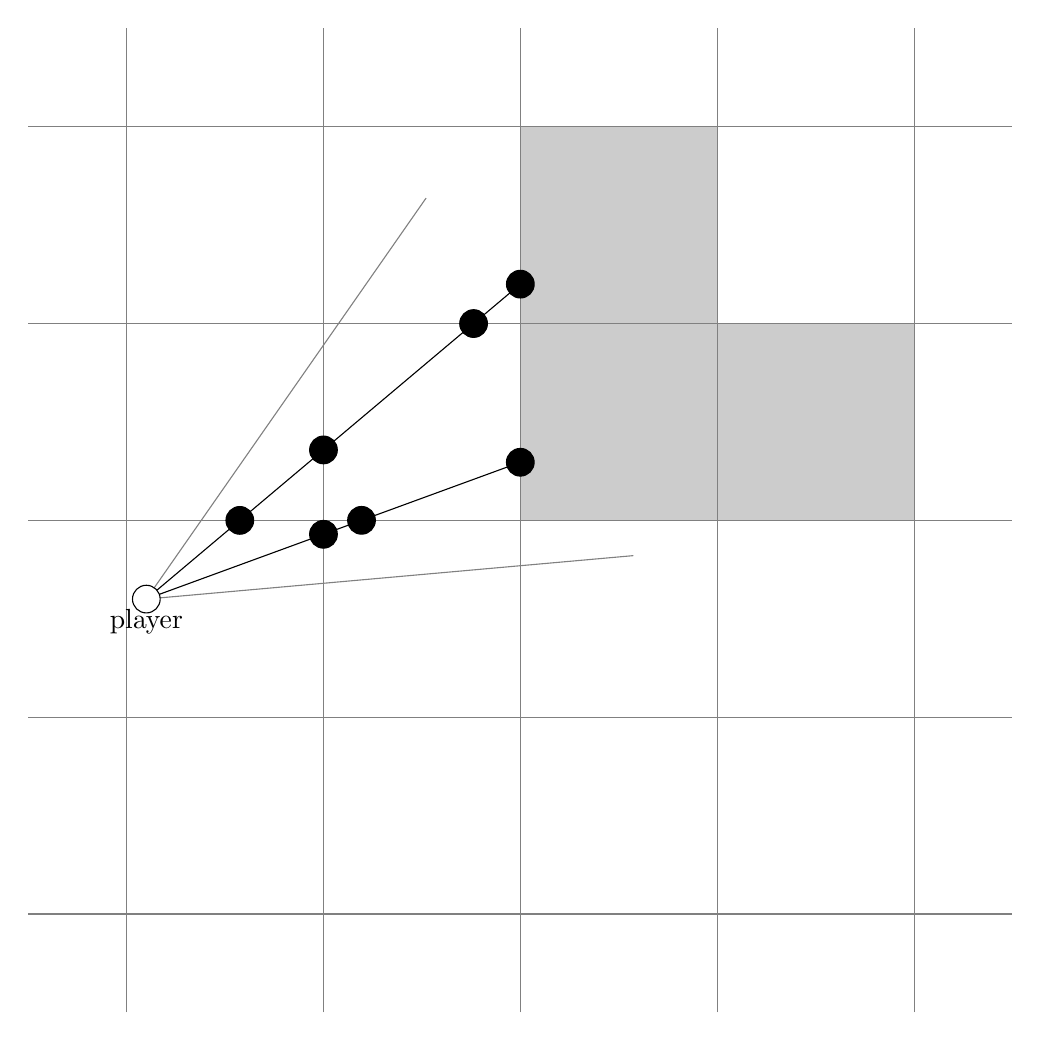
\begin{tikzpicture}[scale=2.5]


\coordinate(player) at (2.1,3.6) {};
\coordinate(intercept) at (4,5.2) {};






\fill[black!20!white, draw=black] (4,5) rectangle (5,6);
\fill[black!20!white, draw=black] (4,4) rectangle (5,5);
\fill[black!20!white, draw=black] (5,4) rectangle (6,5);

%grid
% vertical lines
\draw[draw=gray] (2,1.5) -- (2,6.5) ;
\draw[draw=gray] (3,1.5) -- (3,6.5) ;
\draw[draw=gray] (4,1.5) -- (4,6.5) ;
\draw[draw=gray] (5,1.5) -- (5,6.5) ;
\draw[draw=gray] (6,1.5) -- (6,6.5) ;

% horizontal lines
\draw[draw=gray] (1.5,2) -- (6.5,2) ;
\draw[draw=gray] (1.5,3) -- (6.5,3) ;
\draw[draw=gray] (1.5,4) -- (6.5,4) ;
\draw[draw=gray] (1.5,5) -- (6.5,5) ;
\draw[draw=gray] (1.5,6) -- (6.5,6) ;
%\draw[] 

%FOV
\coordinate[](left_edge) at ($(player)!1!15:(intercept)$);
\coordinate[](right_edge) at ($(player)!1!325:(intercept)$);
\draw[draw=gray] (player) -> (left_edge) ;
\draw[draw=gray] (player) -> (right_edge) ;

\draw[draw=black] (player) -- (intercept) ;

\fill[draw=black] (intercept) circle (2pt);

\draw(player)node[below]{player};

% check points for first intercept
\coordinate(line1_p1) at (0,4) {};
\coordinate(line1_p2) at (9,4) {};
\coordinate (check1) at (intersection of player--intercept and line1_p1--line1_p2);
\fill[draw=black] (check1) circle (2pt);

\coordinate(line2_p1) at (0,5) {};
\coordinate(line2_p2) at (9,5) {};
\coordinate (check2) at (intersection of player--intercept and line2_p1--line2_p2);
\fill[draw=black] (check2) circle (2pt);

%vertical intercelpt
\coordinate(line3_p1) at (3,0) {};
\coordinate(line3_p2) at (3,9) {};
\coordinate (check3) at (intersection of player--intercept and line3_p1--line3_p2);
\fill[draw=black] (check3) circle (2pt);



%intercept 2
\coordinate[](missed_intercept) at ($(player)!1!340:(intercept)$);


\coordinate(i2_line1_p1) at (0,4) {};
\coordinate(i2_line1_p2) at (9,4) {};
\coordinate (i2_check1) at (intersection of player--missed_intercept and i2_line1_p1--i2_line1_p2);
\fill[draw=black] (i2_check1) circle (2pt);

%vertical intercelpt
\coordinate(i2_line2_p1) at (4,0) {};
\coordinate(i2_line2_p2) at (4,9) {};
\coordinate (i2_check2) at (intersection of player--missed_intercept and i2_line2_p1--i2_line2_p2);
\fill[draw=black] (i2_check2) circle (2pt);


\coordinate(i2_line3_p1) at (3,0) {};
\coordinate(i2_line3_p2) at (3,9) {};
\coordinate (i2_check3) at (intersection of player--missed_intercept and i2_line3_p1--i2_line3_p2);
\fill[draw=black] (i2_check3) circle (2pt);
\draw[draw=black] (player) -- (i2_check2) ;

\fill[draw=black, fill=white] (player) circle (2pt);

\end{tikzpicture}
\end{document}

 
\end{figure}
\par
These constraints enable a variant of the DDA algorithm\footnote{Digital differential analyzer}: A fast and accurate way to detect where a ray hits a wall on the map.
\par
In retroscpect a rasterizer approach would a made more sense:\\
\begin{fancyquotes}
\par
Much was made about the "ray casting" used in Wolfenstein, but the real reason for it was that I had a lot of trouble with wall-span rendering in Catacombs 3D.  C3D (and Hovertank before that) shipped with various graphics glitches that you could get in some combinations of map block configurations, position, and viewing angle.  Some were due to fixed point precision issues not being handled optimally, and some were due to clipping and culling issues that I didn't really get a handle on until a couple years later.  In any case, they bothered me a lot.  Spurious graphics glitches do a lot of harm to the sense of immersion in a game, and I very much wanted Id games to feel "rock solid".
 \bigskip \\
There was a clear performance cost to it - doing 320 traces through a tile map and treating each column independently is much slower than looping through a few long wall segments.  However, the resulting code was small and very regular compared to the hairball of my wall span renderers, and it did deliver the rock-solid feel I wanted.
 \bigskip \\
If you made extremely jagged block maps that would turn into many dozen independent wall segments, the ray casting could start to look like a good performance choice, but few scenes were even close to that.  This is exactly the same ray tracing versus rasterization performance tradeoff that is still being made today, but now it is "how many tens of millions of triangles per frame to ray tracing break-even" instead of "how many dozen wall segments".
 \bigskip \\
\textbf{John Carmack - Programmer}
 \end{fancyquotes}



 \par
\begin{figure}[H]
  \centering
 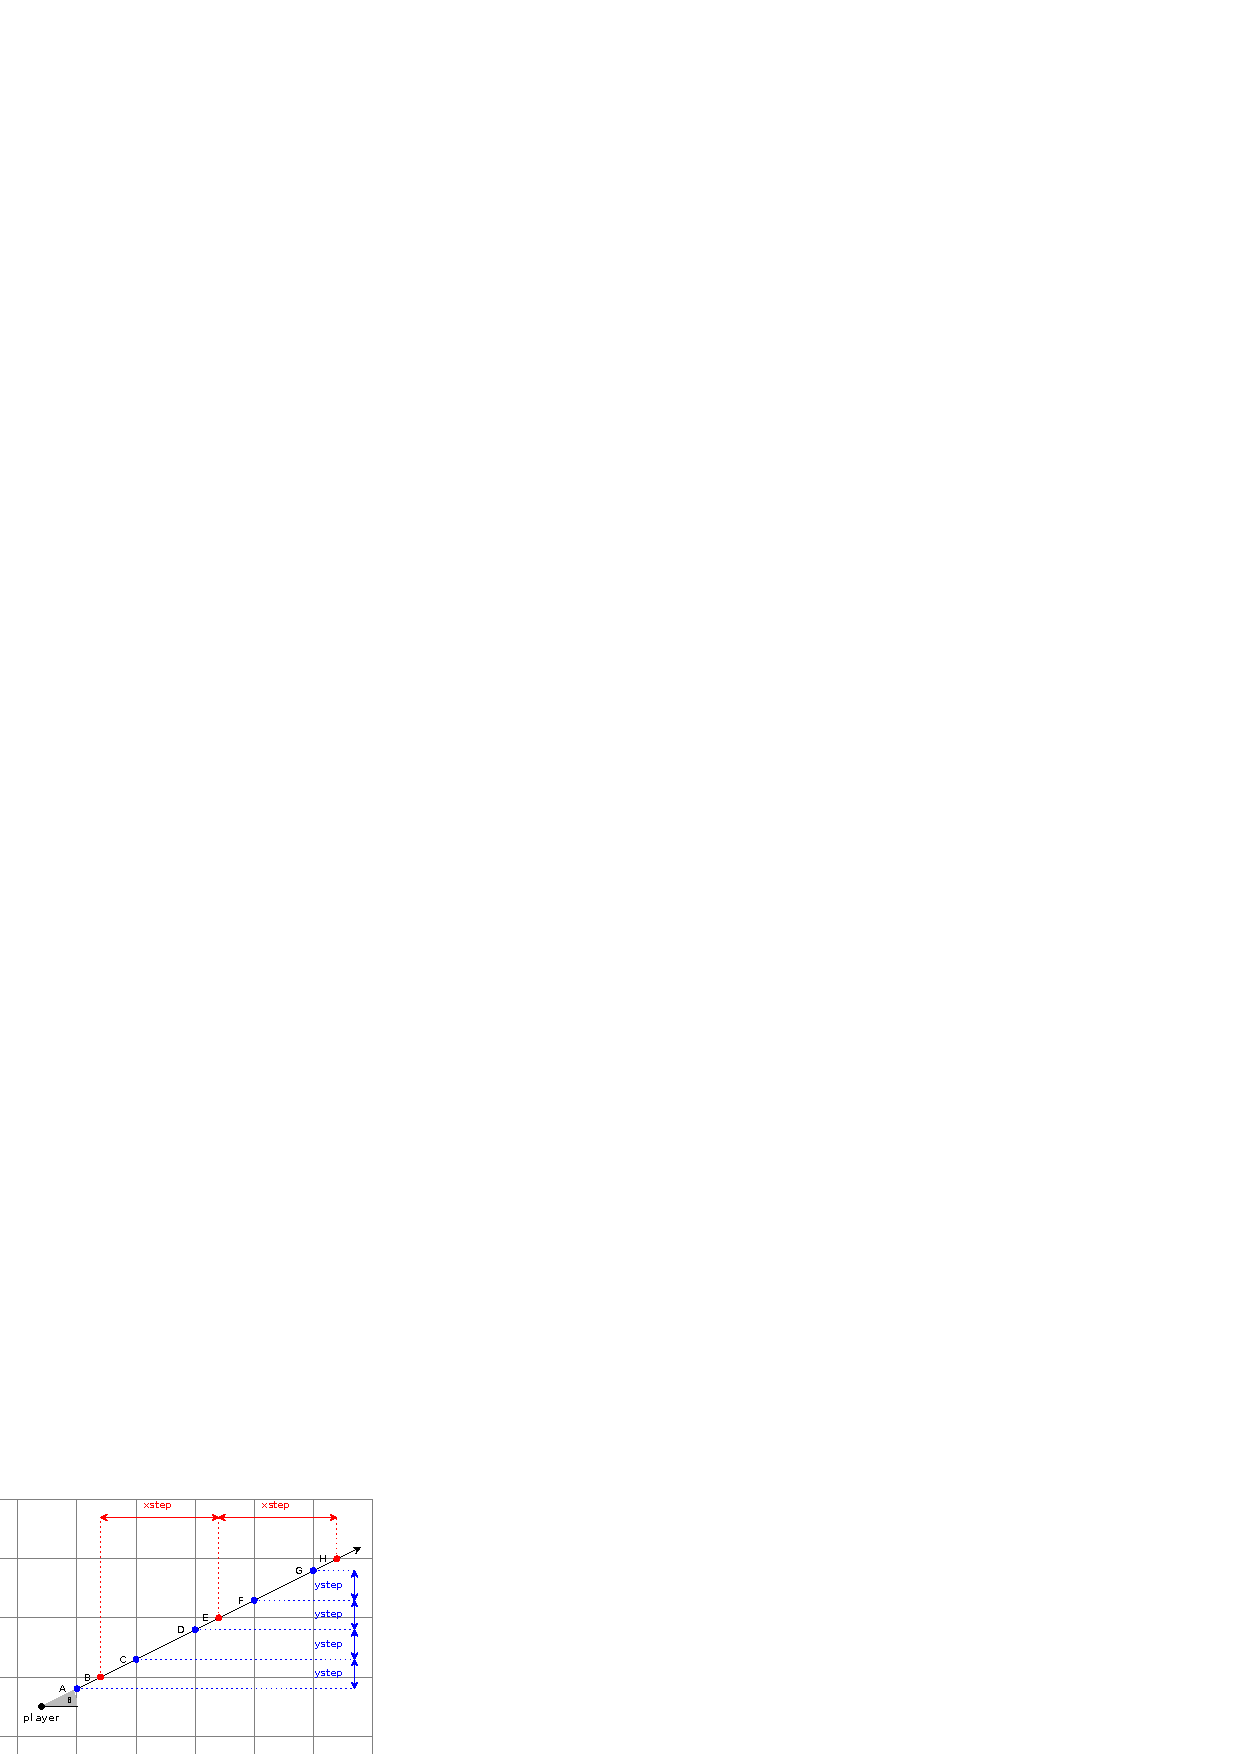
\includegraphics[width=\textwidth]{imgs/drawings/dda.pdf}
\end{figure}
\par
The reason DDA is so fast is because on the first intersection with an axis is known (A for Y axi and B for Y axis on the drawings) all subsequent intersection coordinate are one simple addition away.
\par


\begin{equation*}
    \scalebox{1.3}{
$C = (A.x +1, A.y + xstep)$\\
}
\end{equation*}
\begin{equation*}
    \scalebox{1.3}{
$D = (C.x +1, C.y + xstep)$\\
}
\end{equation*}
\begin{equation*}
    \scalebox{1.3}{
$F = (D.x +1, D.y + xstep)$\\
}
\end{equation*}
\begin{equation*}
    \scalebox{1.3}{
$G = (F.x +1, F.y + xstep)$\\
}
\end{equation*}



In a similar fashion:\\
  \begin{equation*}
    \scalebox{1.3}{

$E = (B.x + ystep, A.y + 1)$\\
}
\end{equation*}
  \begin{equation*}
    \scalebox{1.3}{
$D = (E.x + ystep, E.y + 1)$\\
}
\end{equation*}

This CPU limitation and grid solution bubbled up all the way to the game designer and it explains why all Wolfenstein 3D maps are made of square elements all aligned on axis:\\
\par
\begin{figure}[H]
  \centering
 \fullimage{e1m1.png}
 \caption{The legendary E1M1. Player is the green arrow at the bottom.}
\end{figure}


\subsubsection{Call Apogee}
With map being simple and fast to draw, a contest was to be held: Find a special item in a particularly difficult to access place in the game and call the publisher (Apogee). The maze is located in Episode 2, Map 8:\\
\par
\begin{figure}[H]
  \centering
 \fullimage{e2m8.png}
\end{figure}

\par
Behind a forest of push walls (white squares) and angry bosses (blue star), a sign finally showed up (the red triangle in the map above):\\
\par

\begin{figure}[H]
  \centering
 \fullimage{call_apogee.png}
\end{figure}
\par
However due to people reverse engineering the map format and cheat sites allowing players to find the maze, the sign was replaced with a skeleton with all game shipping during 1992.
\par
\begin{fancyquotes}
"Call Apogee and say Aardwolf."  It's a sign that to this day is something
that I get asked about a lot.  This is a sign that appears on a wall in a
particularly nasty maze in Episode 2 Level 8 of Wolfenstein 3D.  The sign
was to be the goal in a contest Apogee was going to have, but almost
immediately after the game's release, a large amount of cheat and mapping
programs were released.  With these programs running around, we felt that
it would have been unfair to have the contest and award a prize.  The sign
was still left in the game, but in hindsight, probably should have been
taken out.  To this day, Apogee gets letters and phone calls and asking
what Aardwolf is, frequently with the question, "Has anyone seen this yet?"\\
\\
Also, in a somewhat related issue, letters were shown after the highest score
in the score table in some revisions of the game.  These letters were to be
part of another contest that got scrapped before it got started, where we were
going to have people call in with their scores and tell us the code; we'd then
be able to verify their score.  However, with the cheat programs out there,
this got scrapped too.\\
\\
Basically, "Aardwolf" and the letters mean nothing now.  Also note that if
you found the Aardwolf sign in the game (without cheating), there's a VERY
strong chance that you're stuck in there.  The only way out may be to restart,
or load a saved game from before you went into that maze.\\
\\
\textbf{Joe Siegler - Past Pioneers of the Shareware Revolution}
\end{fancyquotes}
\par
\bu{Trivia :} What is Aardwolf? A maned striped mammal (Proteles cristatus) of southern and eastern Africa that resembles the related hyenas and feeds chiefly on carrion and insects. It was back them the mascot of Id, appearing on Tom's Gotta Lists and the Commander Keen 6 Hint Sheet.














 
 
 
 
 
 
 
 
\subsubsection{Raycasting: DDA Algorithm}
The variant of DDA is a fully handcrafted 740 lines of assembly routine \cw{PROC AsmRefresh}. Represented in C for readability it consists of two while looks (one checking vertical intersection and one checking the horizontal) ping-ponging with each other via goto. It is highly unorthodox and super efficient:\\
\par

\par
\begin{figure}[H]
\centering
 % \documentclass[crop,tikz,ifthenelse]{standalone}

% \usetikzlibrary{calc}
% \usepackage{tkz-euclide}
% \usetkzobj{all}


% \begin{document}
\begin{tikzpicture}[scale=2]

\coordinate(origin) at (0,0);
\coordinate(yaxis) at (0,6.5);
\coordinate(xaxis) at (6,0) ;

\draw (0,0) circle (2);
\draw[->,>= latex] (-2.4,0) -- (2.4,0);
\draw[->,>= latex] (0, -2.4) -- (0, 2.4);

// tangent line
\coordinate (tantop) at (2,2.4);
\coordinate (tanbottom) at (2,-2.4);
\draw[->,>= latex] (tanbottom) -- (tantop);

\coordinate (point) at (35:2);
\coordinate (origin) at (0,0);



\node[below left] {\Large $(0,0)$};

\coordinate (procsin) at ($(origin)!(point)!(yaxis)$);
\coordinate (projcos) at ($(origin)!(point)!(xaxis)$) ;

\node[left]  at (procsin) {\Large $sin(\theta)$};
\node[below] at (projcos) {\Large $cos(\theta)$};

\draw[dotted] (projcos) -- (point) ;
\draw[dotted] (procsin) -- (point) ;



\coordinate (extended_point) at (2,1.4);%(35:3);
%\coordinate (tan_point) at (intersection of origin--extended_point and tanbottom -- tantop );

\node[right] at (extended_point) {\Large $tan(\theta)$};

\tkzMarkAngle[fill= gray,size=0.6](xaxis,origin,extended_point);
\tkzLabelAngle[pos = 0.4](extended_point,origin,xaxis){\Large $\theta$};
\draw (origin) -- (extended_point) ;
\end{tikzpicture}
% \end{document}

\end{figure}

\begin{minipage}{\textwidth}
\lstinputlisting[language=C]{code/flipflop.c}
\end{minipage}
This algorithm results in \cw{jmp} heavy instructions but on a an architecture devoid of pipeline and code cache such as the 386 it is not a problem at am.\\
\bu{Trivia:} To accelerate \cw{cos}, \cw{sin} and \cw{tan} calculation, the engine uses lookup table: One entry for each 360 degres.





















\subsubsection{Calculate column height}
Before proceeding to the next session about fish eye projection correction, here is a reminder of something we all learned in highschool: SOH-CAH-TOA.

 \begin{fancyquotes}
  I'm no super mathematician-- I learned high school math well enough to solve real world problems with it.\\
 \par
\textbf{John Carmack - Programmer}
 \end{fancyquotes}


\par
\begin{figure}[H]
\centering
 % \documentclass{standalone}% 'crop' is the default for v1.0, before it was 'preview'
% \usepackage[x11names,dvipsnames]{xcolor} %Colocação de cores
% \usepackage{tikz,tikz-3dplot} %Para fazer desenhos
% \usepackage{tkz-euclide}
% \usetkzobj{all}
\begin{tikzpicture}[scale=1.5]

% \begin{document}
% \begin{tikzpicture}[]

\coordinate(A) at (0,0);
\coordinate(B) at (7,0);
\coordinate(C) at (0,5);

\draw[draw=black] (A) -- node[below] {\Large A} (B);
\draw[draw=black] (B) -- node[above] {\Large H} (C);
\draw[draw=black] (C) -- node[left] {\Large O} (A);

\tkzMarkRightAngle(B,A,C);
\tkzLabelAngle[pos = 1.0](A,B,C){\Large $\alpha$}
\tkzMarkAngle[fill= gray,size=1.8cm,opacity=.2](C,B,A)

\node (A) at (7.5,3.5) {\Large $sin(\alpha) = \frac{O}{H}$};
\node (A) at (7.5,2.5) {\Large $cos(\alpha) = \frac{A}{H}$};
\node (A) at (7.5,1.5) {\Large $tan(\alpha) = \frac{O}{A}$};

\end{tikzpicture}
%\end{document}
\end{figure}



This property is multiple places:\\
This is all you need to understand fish eye correction and coordinate projection (used to place player, and calculate sounds).

\par
Once a ray has hit a wall (from coordinate (\cw{viewx},\cw{viewy} to (\cw{xintercept},\cw{yintercept}) it is time to calculate how tall the 
column of pixel should be. This happens in function \cw{CalcHeight}:\\

\begin{minipage}{\textwidth}
\lstinputlisting[language=C]{code/CalcHeight.c}
\end{minipage}

The code is not what one would expect: The raycasting algorithm is supposed to cast a ray for each pixel column and use the distance \codeword{d} to infer the column's height on screen. So one would have expected to see a formula like:
\begin{figure}[H]
  \centering
  \begin{equation*}
    \scalebox{1.3}{
$ d = \sqrt{dx^2 + dy^2}$ 
 }
  \end{equation*}
\end{figure}
But instead the code looks like it is doing: 
\begin{figure}[H]
  \centering
  \begin{equation*}
    \scalebox{1.3}{
$d = dx * \cos(\alpha) - dy * \sin(\alpha) $
 }
  \end{equation*}
\end{figure}
Something is fishy here. Let's explain with an example:\\
\par
\begin{figure}[H]
\centering
 %\documentclass[tikz,border=2pt,png]{standalone}
%\usepackage{tkz-euclide}
%\usetkzobj{all}
%\begin{document}
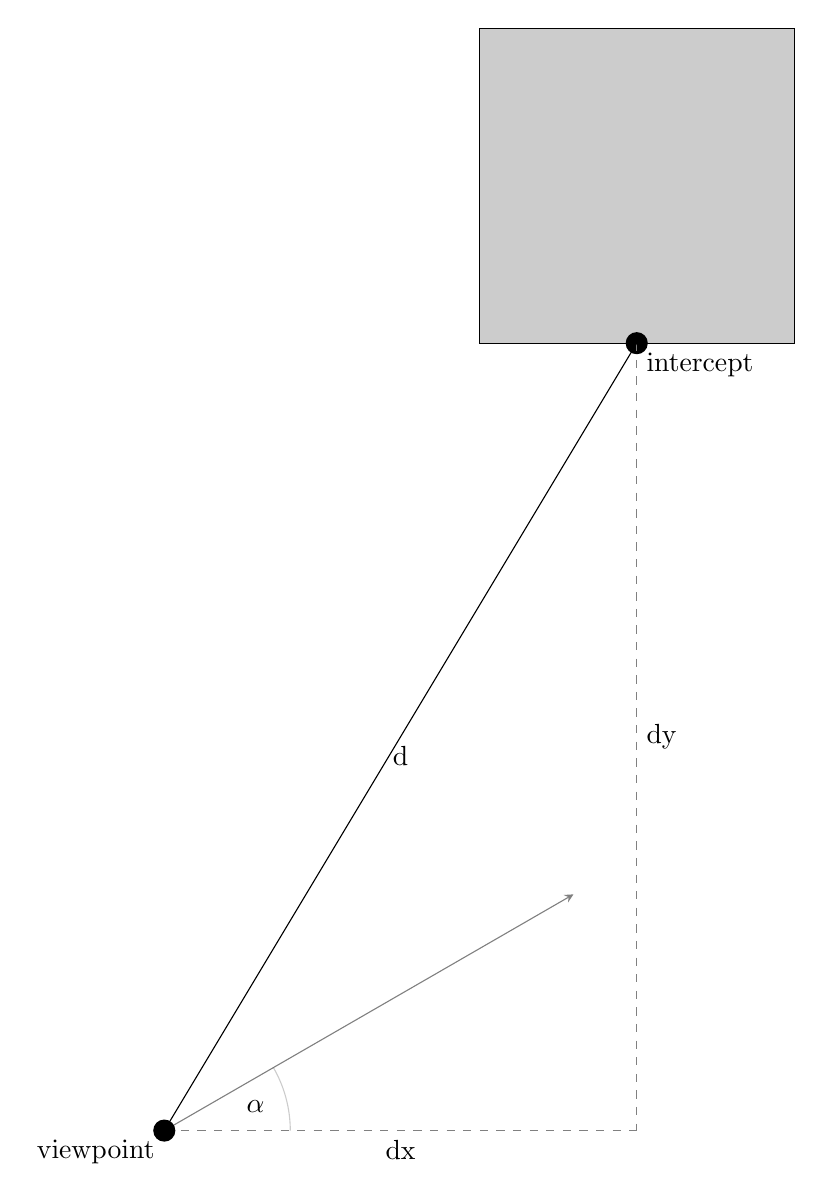
\begin{tikzpicture}[scale=2.0]

\coordinate(origin) at (0,0)[label=below:view] {};
\coordinate(yaxis) at (0,6.5){};
\coordinate(xaxis) at (6,0) {};
\coordinate(angle) at (30:3);
\coordinate(intercept) at (3,5) {};

\node[below left] (orign) {viewpoint};
\node[below right] (_XX) at (intercept) {intercept};

% AXIS
%\draw[->,draw=black,>=stealth] (origin)  -- (xaxis) ;
%\draw[->,draw=black,>=stealth] (origin)  -- (yaxis) ;
%\draw[draw=black] (origin)  -- (0,-0.5) ;
%\draw[draw=black] (origin)  -- (-0.5,0) ;

% WALL
\fill[black!20!white, draw=black] (2,5) rectangle (4,7);
%\fill[black!20!white, draw=black] (4,5) rectangle (6,7);
%\fill[black!20!white, draw=black] (4,3) rectangle (6,5);


\fill (intercept) circle (2pt);


\draw[->,draw=gray,>=stealth] (origin)  -- (angle) ;

\coordinate (dx) at ($(origin)!(intercept)!(xaxis)$);
\draw[draw=gray,>=stealth,dashed] (origin) -- node[below] {dx} (dx);
\draw[draw=gray,>=stealth,dashed] (intercept) -- node[right] {dy}(dx);

\tkzMarkAngle[fill= gray,size=0.8cm,opacity=.2](xaxis,origin,angle)
\tkzLabelAngle[pos = 0.6](xaxis,origin,angle){$\alpha$}

\fill[fill=black] (origin) circle (2pt);

\draw[] (origin) -- node[below] {d} ++(intercept) ;

%\draw[] 


\end{tikzpicture}
%\end{document}
 \caption{Raycasting using distance d} \label{fig:Raycasting2}
\end{figure}

In this drawing the player is located at viewpoint with a view angle \begin{math}\alpha\end{math}. A ray has been cast from \cw{viewpoint} and it hit a wall at \cw{intercept}. The distance \codeword{d} is a straight line between the player point of view and the location where the ray hit the line which can be obtained with $d = \sqrt{dx^2 + dy^2}$. Repeated for all rays, such an algorithm would result in a "fisheye effect".

\begin{figure}[H]
\centering
  \fullimage{fish_eye/bad_mild.png}
 \caption{Fish eye effect: Mild}. \label{fig:mips}
 \end{figure}








\begin{minipage}{.5\textwidth}
To demonstrate the fish eye distorstion we will show three screenshots of a modified version of the engine. it was altered to use distance \cw{d} instead of "something else" to calculate column heights. In the next three screenshots the player get progressively closer to a wall. At first the distorsion is barely noticeable.
 \end{minipage}
\begin{minipage}{.5\textwidth}
\begin{figure}[H]
  \begin{flushright}
 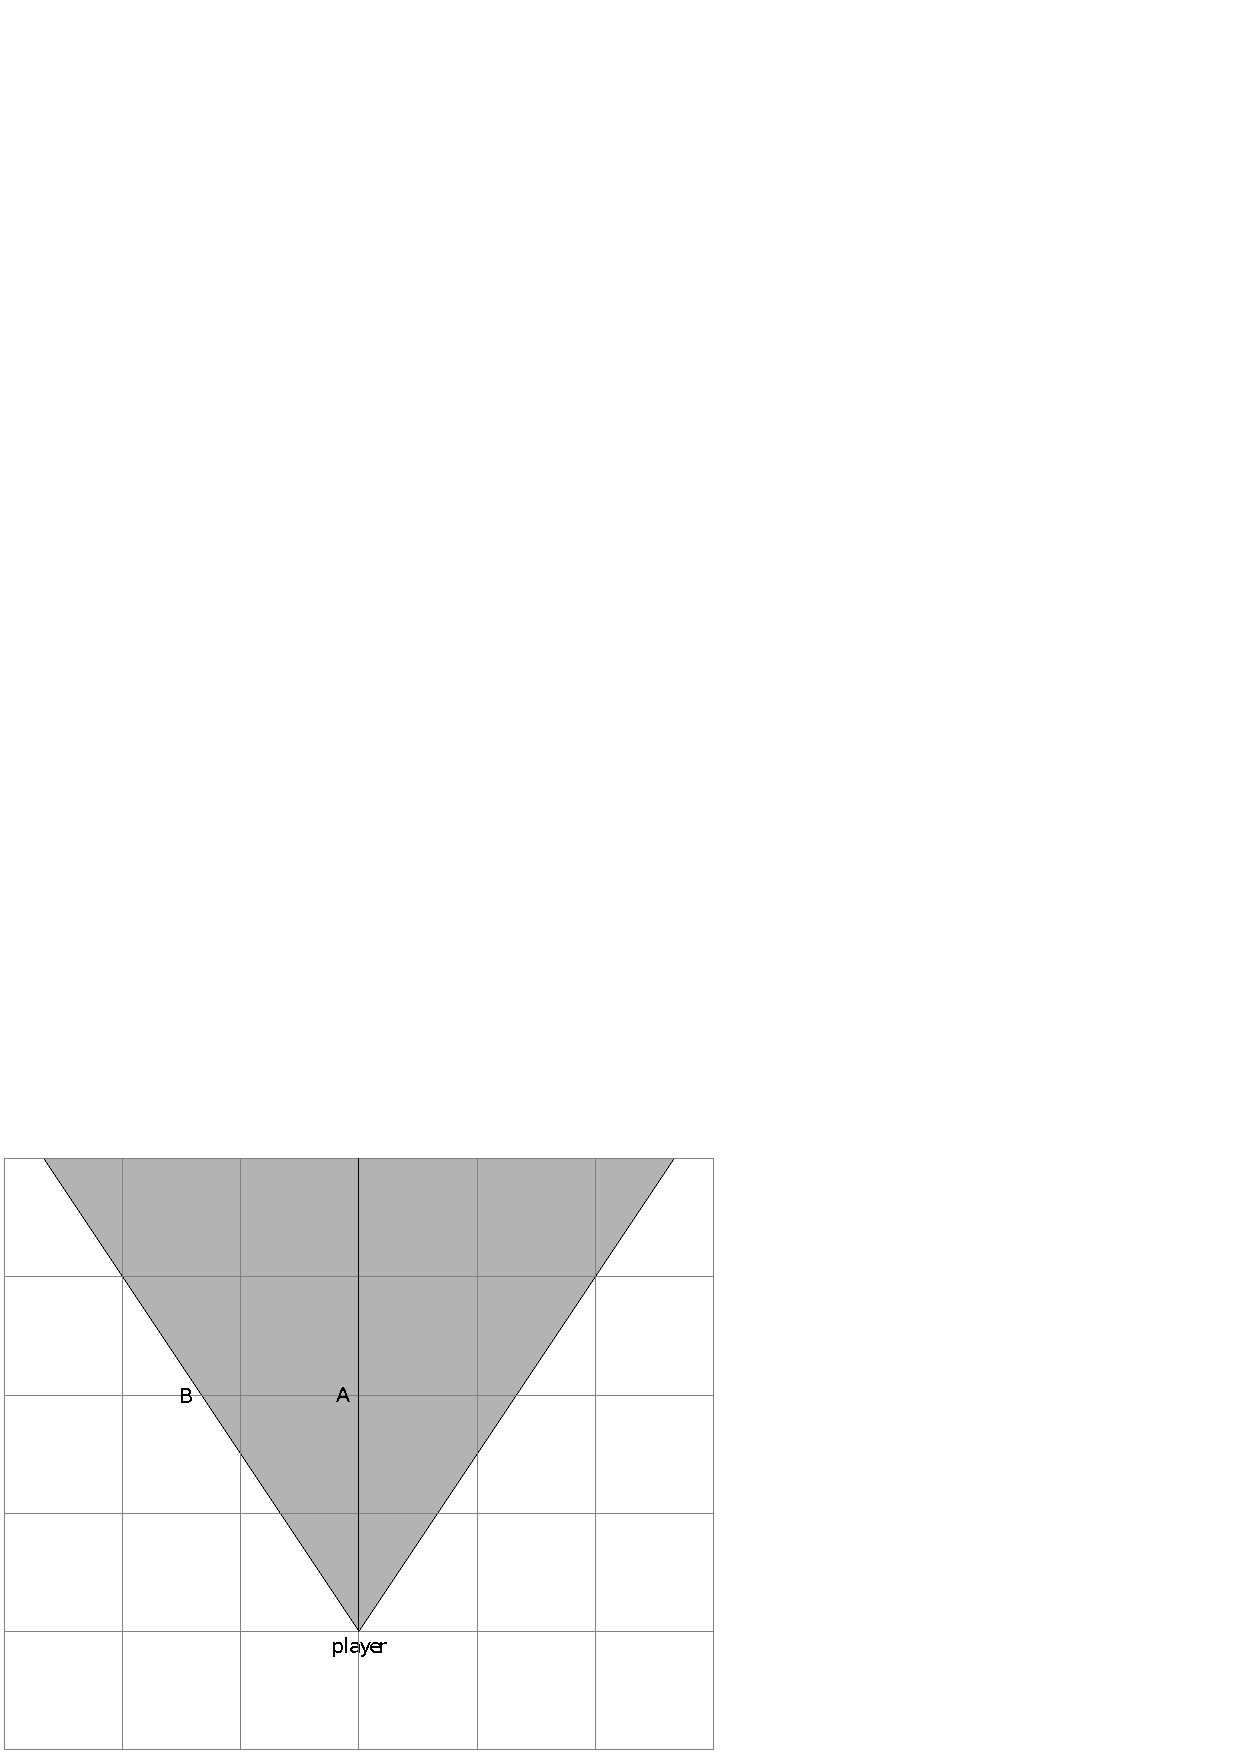
\includegraphics[width=.9\textwidth]{imgs/drawings/fish_eye/top_view_far.pdf}
   \end{flushright}
\end{figure}
\end{minipage}

\par




\begin{figure}[H]
\centering
  \fullimage{fish_eye/bad_ok.png}
 \caption{Fish eye effect: Bad} \label{fig:mips}
 \end{figure}




\begin{minipage}{.5\textwidth}
At a distance of 24 feet, the distorstion cannot be ignored. Note that even though the player is getting closer to the wall, the ratio of A and B remain the same. The absolute difference however becomes noticeable.
 \end{minipage}
\begin{minipage}{.5\textwidth}
\begin{figure}[H]
  \begin{flushright}
 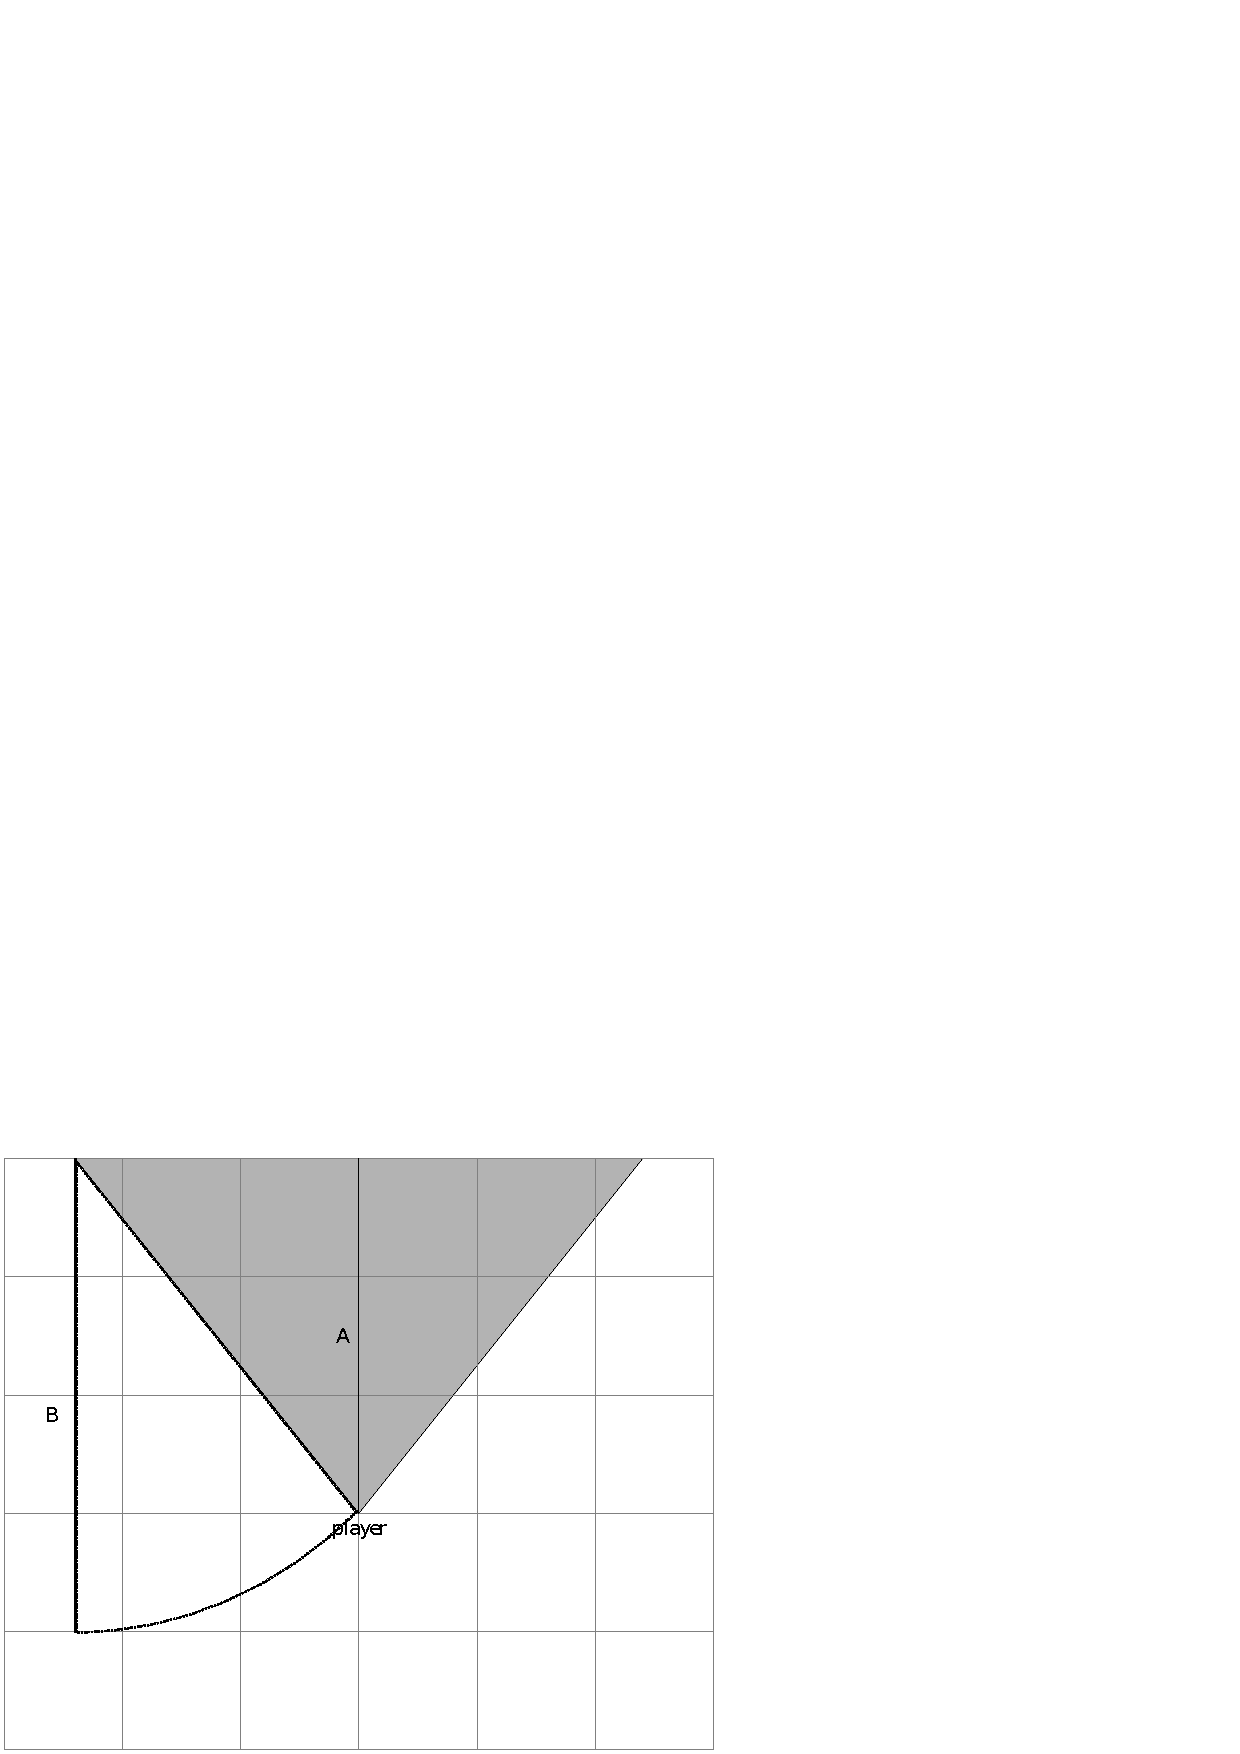
\includegraphics[width=.9\textwidth]{imgs/drawings/fish_eye/top_view_middle.pdf}
 \end{flushright}
\end{figure}
\end{minipage}






 \begin{figure}[H]
\centering
  \fullimage{fish_eye/bad_bad.png}
 \caption{Fish eye effect: AAAAARG} \label{fig:mips}
 \end{figure}
 

\begin{minipage}{.5\textwidth}
At close range (8 feet) the distorsion is straight up unpleasant. To avoid this distortion and get a more pleasant rendition, what must be used is not the direct distance \cw{d} but \cw{d} projected on the perpendicular of the view direction (\cw{z}):
 \end{minipage}
\begin{minipage}{.5\textwidth}
 \begin{figure}[H]
  \begin{flushright}
  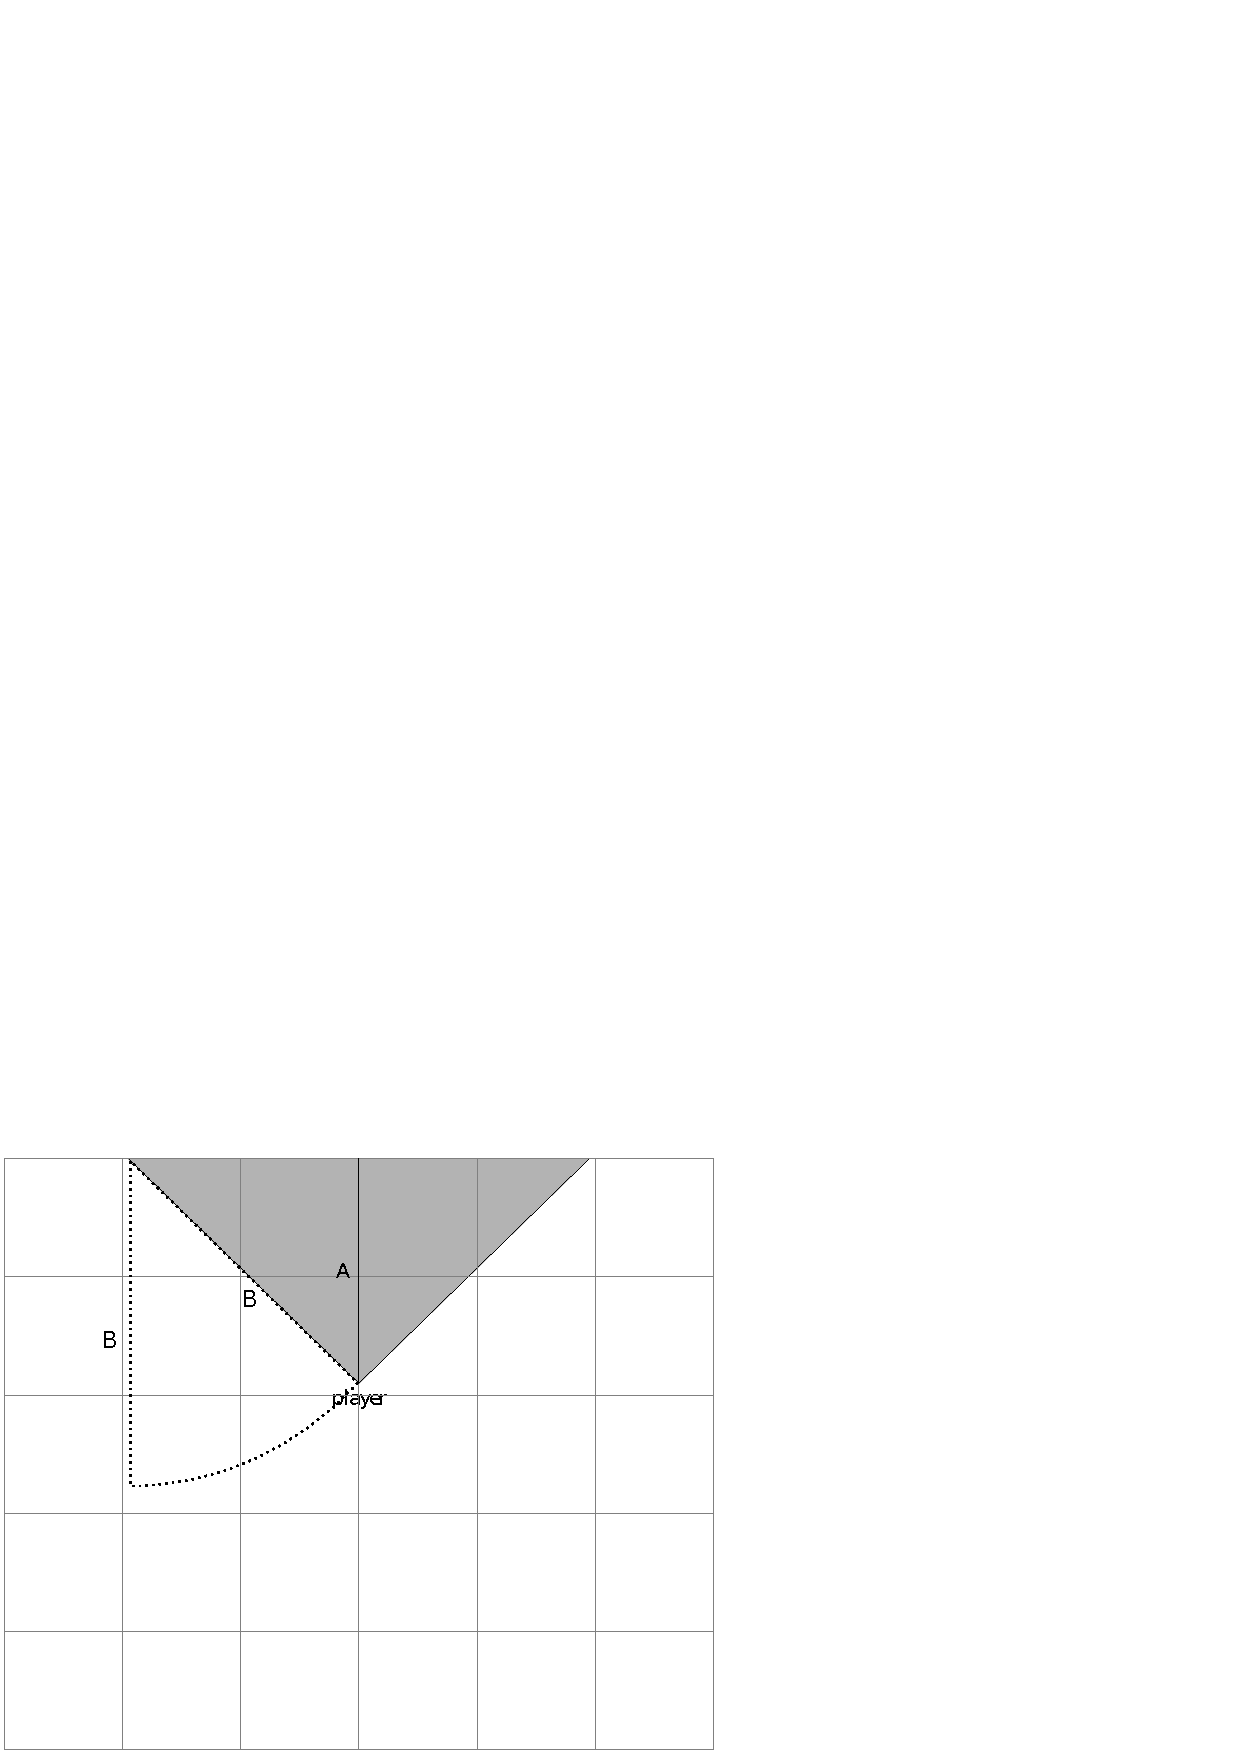
\includegraphics[width=.9\textwidth]{imgs/drawings/fish_eye/top_view_close.pdf}
 \end{flushright}
\end{figure}
 \end{minipage}

\par



\begin{figure}[H]

 %\documentclass[tikz,border=2pt,png]{standalone}
%\usepackage{tkz-euclide}
%\usetkzobj{all}
%\begin{document}
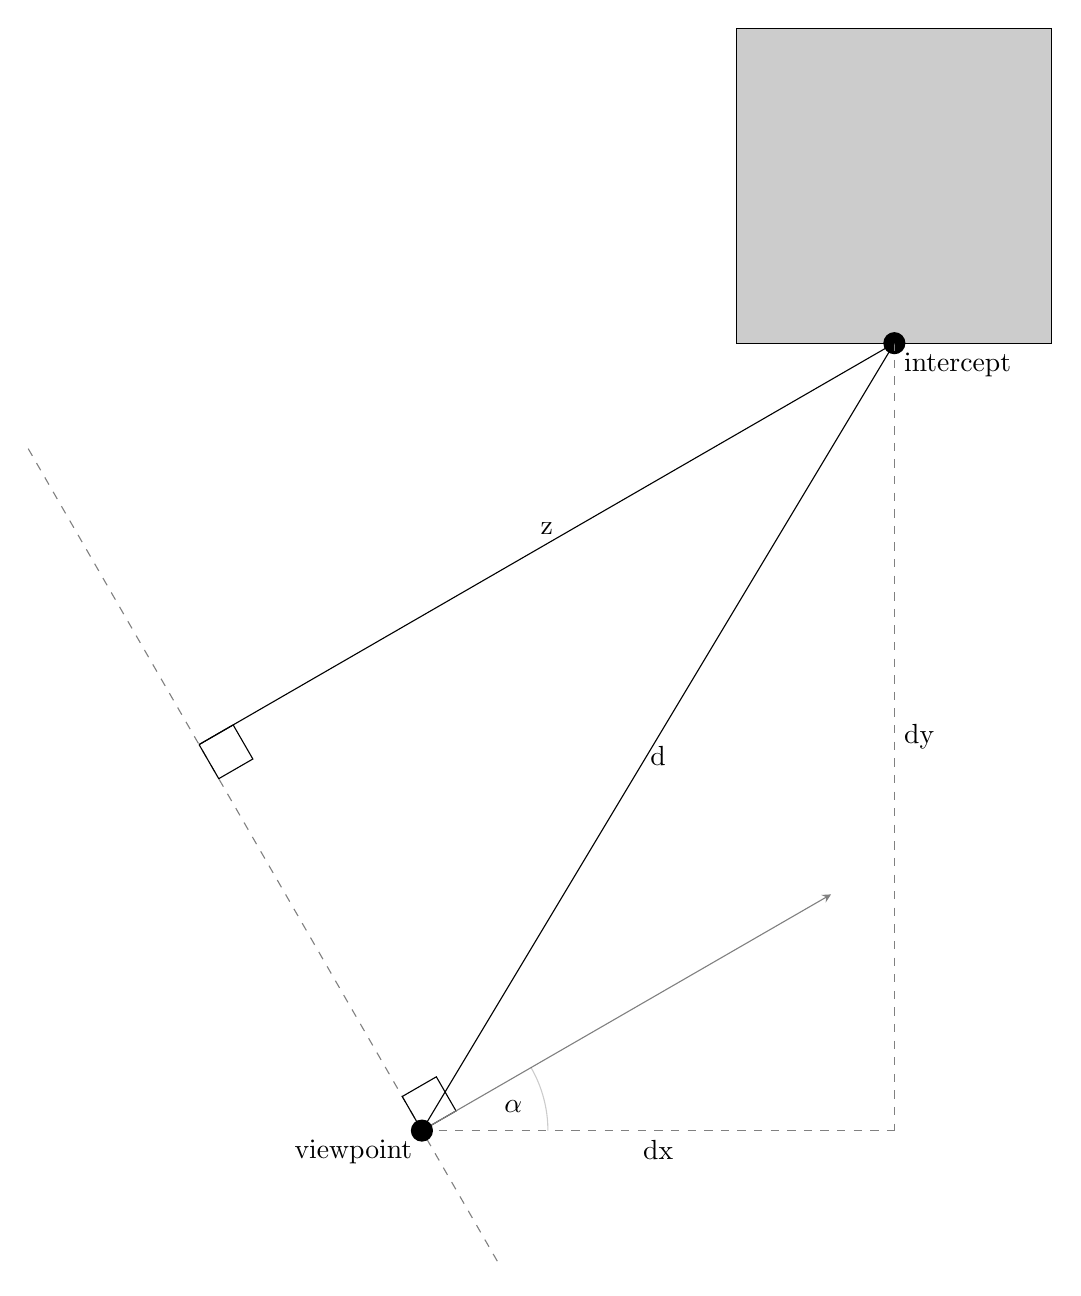
\begin{tikzpicture}[scale=2.0]

\coordinate(origin) at (0,0)[label=below:view] {};
\coordinate(yaxis) at (0,6.5){};
\coordinate(xaxis) at (6,0) {};
\coordinate(angle) at (30:3);
\coordinate(intercept) at (3,5) {};

\node[below left] (orign) {viewpoint};
\node[below right] (_XX) at (intercept) {intercept};

% plan
\coordinate(planA) at (120:5);
\coordinate(planB) at (-60:1);
\draw[draw=gray,dashed] (planA) -- (planB);
% AXIS
%\draw[->,draw=black,>=stealth] (origin)  -- (xaxis) ;
%\draw[->,draw=black,>=stealth] (origin)  -- (yaxis) ;
%\draw[draw=black] (origin)  -- (0,-0.5) ;
%\draw[draw=black] (origin)  -- (-0.5,0) ;

% WALL
\fill[black!20!white, draw=black] (2,5) rectangle (4,7);
%\fill[black!20!white, draw=black] (4,5) rectangle (6,7);
%\fill[black!20!white, draw=black] (4,3) rectangle (6,5);

% projected intercept
\coordinate (proj_intercept) at ($(planA)!(intercept)!(planB)$);
\draw[draw=black] (proj_intercept) -- node[above] {z} (intercept);

\tkzMarkRightAngle(intercept,proj_intercept,origin);
\tkzMarkRightAngle(angle,origin,proj_intercept);

\fill (intercept) circle (2pt);

% Angle
\draw[->,draw=gray,>=stealth] (origin)  -- (angle) ;

\coordinate (dx) at ($(origin)!(intercept)!(xaxis)$);
% DX and DY
\draw[draw=gray,>=stealth,dashed] (origin) -- node[below] {dx} (dx);
\draw[draw=gray,>=stealth,dashed] (intercept) -- node[right] {dy}(dx);

\tkzMarkAngle[fill= gray,size=0.8cm,opacity=.2](xaxis,origin,angle)
\tkzLabelAngle[pos = 0.6](xaxis,origin,angle){$\alpha$}

\fill[fill=black] (origin) circle (2pt);

% D libe
\draw[] (origin) -- node[below] {d} ++(intercept) ;

%\draw[] 


\end{tikzpicture}
%\end{document}
 \caption{blabla.} \label{fig:Raycasting2}
 
\end{figure}

This projection (z) is mathematically hard to calculate in one go (especially with fixed point). The trick is to break it down in two components and use the highschool mnemonic: SOH-CAH-TOA.\\


\begin{figure}[H]
\centering
 %\documentclass[tikz,border=2pt,png]{standalone}
%\usepackage{tkz-euclide}
%\usetkzobj{all}
%\begin{document}
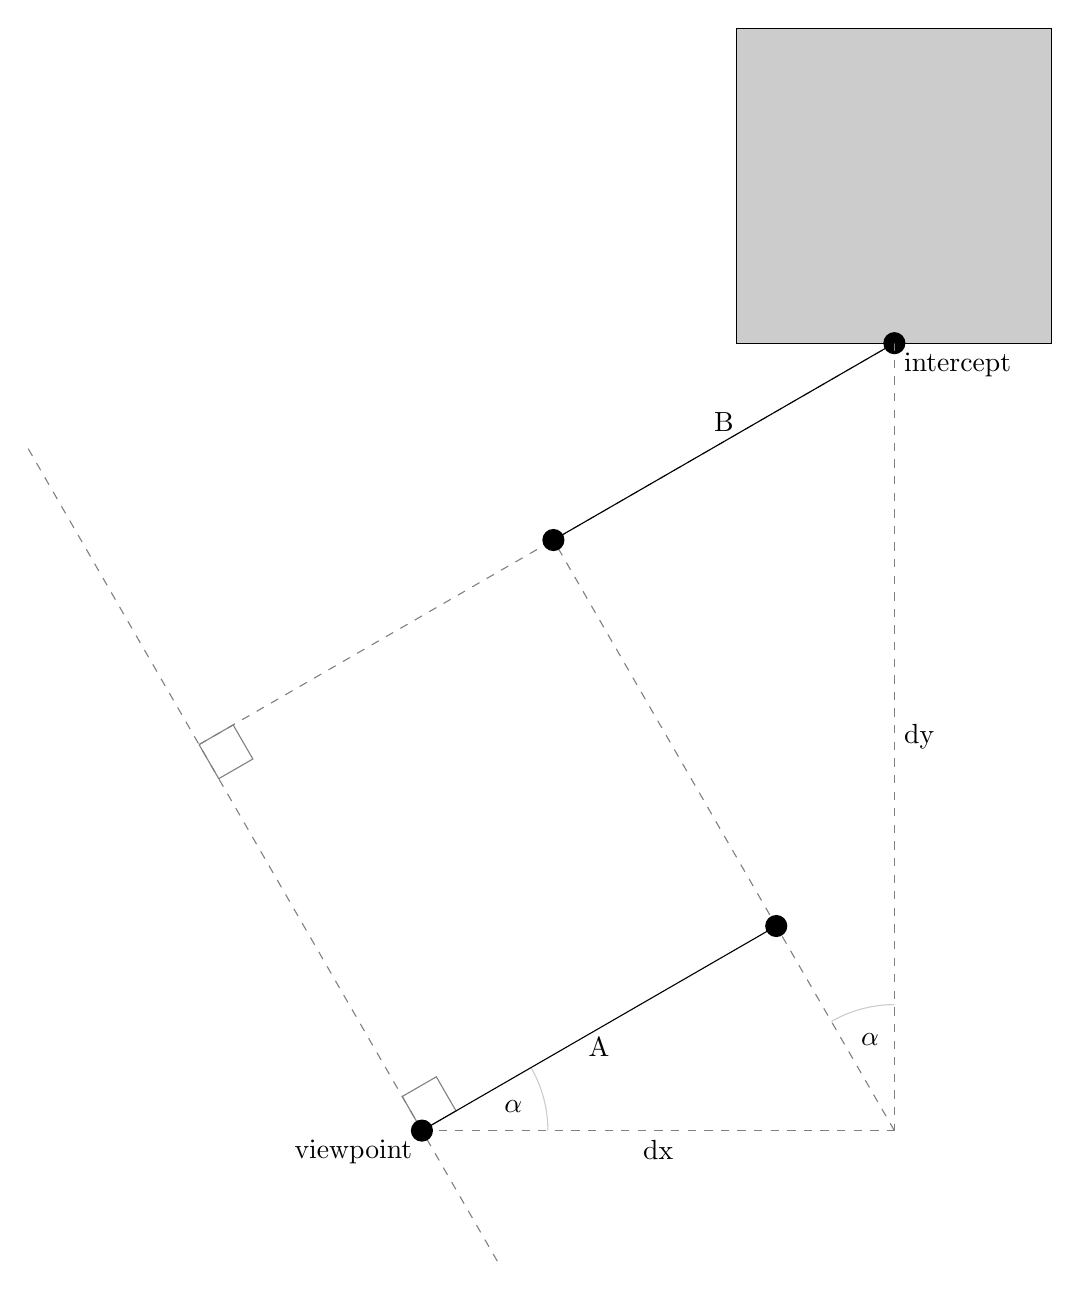
\begin{tikzpicture}[scale=2.0]

\coordinate(origin) at (0,0)[label=below:view] {};
\coordinate(yaxis) at (0,6.5){};
\coordinate(xaxis) at (6,0) {};
\coordinate(angle) at (30:3);
\coordinate(intercept) at (3,5) {};

\node[below left] (orign) {viewpoint};
\node[below right] (_XX) at (intercept) {intercept};

% plan
\coordinate(planA) at (120:5);
\coordinate(planB) at (-60:1);
\draw[draw=gray,dashed] (planA) -- (planB);
% AXIS
%\draw[->,draw=black,>=stealth] (origin)  -- (xaxis) ;
%\draw[->,draw=black,>=stealth] (origin)  -- (yaxis) ;
%\draw[draw=black] (origin)  -- (0,-0.5) ;
%\draw[draw=black] (origin)  -- (-0.5,0) ;

% WALL
\fill[black!20!white, draw=black] (2,5) rectangle (4,7);
%\fill[black!20!white, draw=black] (4,5) rectangle (6,7);
%\fill[black!20!white, draw=black] (4,3) rectangle (6,5);

% projected intercept
\coordinate (proj_intercept) at ($(planA)!(intercept)!(planB)$);
\draw[draw=gray,dashed] (proj_intercept) -- node[above] {} (intercept);

\tkzMarkRightAngle[draw=gray](intercept,proj_intercept,origin);
\tkzMarkRightAngle[draw=gray](angle,origin,proj_intercept);

\fill (intercept) circle (2pt);

% Angle
%\draw[->,draw=gray,>=stealth] (origin)  -- (angle) ;

\coordinate (dx) at ($(origin)!(intercept)!(xaxis)$);
% DX and DY
\draw[draw=gray,>=stealth,dashed] (origin) -- node[below] {dx} (dx);
\draw[draw=gray,>=stealth,dashed] (intercept) -- node[right] {dy}(dx);

\tkzMarkAngle[fill= gray,size=0.8cm,opacity=.2](xaxis,origin,angle)
\tkzLabelAngle[pos = 0.6](xaxis,origin,angle){$\alpha$}

\fill[fill=black] (origin) circle (2pt);

\coordinate (A) at ($(origin)!(dx)!(angle)$);
\draw[] (origin)  -- node[below] {A} (A) ;

\coordinate (B) at ($(proj_intercept)!(dx)!(intercept)$);
\draw[] (intercept)  -- node[above] {B} (B) ;

\draw[draw=gray,dashed] (dx) -- (B) ;

\fill (A) circle (2pt);
\fill (B) circle (2pt);

\tkzMarkAngle[fill= gray,size=0.8cm,opacity=.2](intercept,dx,A)
\tkzLabelAngle[pos = 0.6](intercept,dx,A){$\alpha$}

\end{tikzpicture}
%\end{document}
 
\end{figure}
Using CAH gives $A = dx * \cos(\alpha)$ and SOH gives $B = dy * \sin(\alpha) $. So:



The overall operation can be seen as a rotation of y intercept around the viewpoint.\\
 Which is enough to give pleasant straigh lines. Following a wall uncorrected and the same location with projected distance:


 \begin{figure}[H]

 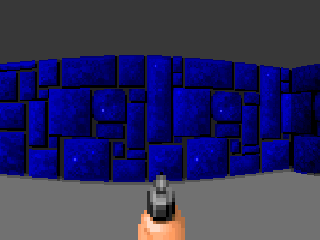
\includegraphics[width=\textwidth]{screenshots/fish_eye/fish_eye.png}
  \caption{Fish eye: Uncorrected} 
  
 \end{figure}
\par
\begin{figure}[H]
  \centering
  \begin{equation*}
    \scalebox{1.3}{
$d = A + B = dx * \cos(\alpha) + dy * \sin(\alpha) $. 
 }
  \end{equation*}
\end{figure}
But since dx and dy are not distances but vectors (with a sign) the equation becomes 


\begin{figure}[H]
  \centering
  \begin{equation*}
    \scalebox{1.3}{
$d = A + B = dx * \cos(-\alpha) + dy * \sin(-\alpha) $ 
 }
  \end{equation*}
\end{figure}
which simplified becomes: 

\begin{figure}[H]
  \centering
  \begin{equation*}
    \scalebox{1.3}{
$d = A + B = dx * \cos(\alpha) - dy * \sin(\alpha) $
 }
  \end{equation*}
\end{figure}
\par
For people who like equations, the overall operation can be seen as the multiplication of a rotation matrix with the vector intercept (dx,dy), which transforms coordinate from map space (origin in upper left corner with axis aligned with the map) to player space (origin at player position with axis aligned with player orientation).
\begin{figure}[H]
  \centering
  \begin{equation*}
    \scalebox{1.3}{
    $
      \begin{bmatrix} 
        \cos(\alpha) & -\sin(\alpha) \\ 
        \sin(\alpha) & \cos(\alpha) 
      \end{bmatrix} 
       *
      \begin{bmatrix} 
        dx \\ 
        dy 
      \end{bmatrix}
       =
      \begin{bmatrix} 
        dx*\cos(\alpha) - dy*\sin(\alpha) \\ 
        dx*\sin(\alpha) + dy*\cos(\alpha) 
      \end{bmatrix} 
      $
    }
  \end{equation*}
\end{figure}

\begin{figure}[H]
\centering
 \includegraphics[width=\textwidth]{imgs/drawings/spaces.pdf}
 \end{figure}


I personally find the graphic explanation with SOH-CAH-TOA much more clear!
\par

 Which is enough to give pleasant straight lines. Following a wall uncorrected and the same location with projected distance:\\

 \begin{minipage}{\textwidth}
 
\centering
  \scaledimage{0.9}{fish_eye/fish_eye.png}
\vspace*{0.5cm}
\centering
  \scaledimage{0.9}{fish_eye/fish_eye_corrected.png}


 \end{minipage}


 \par
 
 \begin{minipage}{\textwidth}
\centering
  \scaledimage{0.9}{fish_eye/fish_eyed_start_screen2.png}
\vspace*{0.5cm}
\centering
 \scaledimage{0.9}{wolf3d_7_fullframe.png}
\end{minipage}

 \par
 \bu{Note :} Why subtract values instead of adding them ? The coordinate system has its origin at the upper left which inverse the vertical axis and therefore the sin value. To compensate for it, the formula subtract the negative value, resulting in an addition.













\subsection{Drawing walls}
Drawing the wall column for each rays may sound easy but it is in fact difficult. It is not hard in terms of mathematics but hard in terms of instructions clock consumption. To scale a texture of 64 pixels tall on the screen centered vertically is expensive. It turns out if you want to do it fast you need a few optimization. This part is where wolfenstein 3d took off and left other 3d engine in the dust. This is the part where lies the two secrets of the engine speed: Compiled scalers and deferred column rendering.\\
\par

\subsubsection{Compiled scalers}
With a distance available for a column, the engine is able to calculate a corresponding pixel height. All columns of pixels representing the walls are centered vertically and either magnified or minified. The goal of the exercice is to scale as fast as possible a column of 64 pixels to any height ranging from 2 pixels to max view height (152 pixels):\\
\par
 \begin{figure}[H]
\centering
 \fullimage{scaler_valign.png}
 \caption{As the added pink line show, every column of pixels are centered vertically. There is no horizontal placing.}
 \end{figure}
\par

\par
 The naive approach would be to use a generic routine with the following prototype:\\


\par
\begin{minipage}{\textwidth}
\lstinputlisting[language=C]{code/generic_draw.c}
\end{minipage}

\par
But that would be a lot of instruction due mostly to the genericity of the function: Indeed it can accept any height from \cw{0} to \cw{INT\_MAX}. But there is a faster way and it involves the eternal RAM vs speed tradeoff: Pre-generate x86 code specialized to drawing all height of wall from 1 pixels to 200 (the height of the screen).\\
\par
\begin{minipage}{\textwidth}
\lstinputlisting[language=C]{code/compscale.c}
\end{minipage}

\par
What is the cost of the precompiling these scalers? How much RAM does it use? It takes 7 instructions of one byte each to write a pixel. So if all size were generated from 2,4,6...152, we could use Gauss method to calculate the size:\\
\par
$154*38*7=40,964$ bytes\\
\par
That cost was deemed too high, so past size 76 only every other size are generated (2,4,6,,..,72,74,76) and (78,82,86,...,144,148,152):\\
\par
$78*19*7+9*230*7=26,474$ bytes\\
\par











\subsubsection{Deferred column drawing}
There is a second level of tricks to draw a column of pixel. A naive raycaster/compiled scaler coupling would look like this:\\

\begin{minipage}{\textwidth}
\lstinputlisting[language=C]{code/naive_raycaster_pseudocode.c}
\end{minipage}
\par
But the engine is not done this way. Instead it buffers what to draw:\\
\par
\begin{minipage}{\textwidth}
\lstinputlisting[language=C]{code/wolf3d_raycaster_pseudocode.c}
\end{minipage}

\par
The important thing to understand with this approach is that if a ray is deemed similar enough to the last casts, the height
is not calculated again. Instead if uses the same height as the other similar rays. Allowing itself to cheat a little bit introduce a little distortion but unlock formidable speed up: now the engine can write multiple column (up to eight) simulatenously.\par
To understand how this work, let's take a look at a frame and how it is stored in the VGA banks.
 \par


  \begin{minipage}{\textwidth}
 
\centering
  \scaledimage{0.9}{vga_layout/wolf3d_7.png}
\vspace*{0.5cm}
\centering
  \scaledimage{0.9}{vga_layout/wolf3d_7_bank.png}


 \end{minipage}
Notice how column representing wall are at the same address in the banks. Leveraging the VGA mask allowing to write in multiple banks at the same time, it is possible to render column of pixels simultaneously. But this is only done when the distortion would not be too noticeable. Columns of wall must be deemed similar enough. Now the interesting question is: What makes rays similar? The answer is two rays hiting the same wall and resulting in the same
texture coordinate.
\par

That is theory. In practice the engine must be very careful. The engine allows itself to cheat and render up to eight column at the same height. But it means factoring in the four bytes alignment. The details of this are in the method \codeword{ScalePost} in \codeword{WL\_DRAW.C}.\\

Note: A \quotes{post} is a column of pixel belonging to a wall.\\
ScalePost is written in assembly and performs a maximum of three pass to draw a maximum of eight columns of pixels.\\
\par 
\begin{minipage}{\textwidth}
\lstinputlisting[language=C]{code/ScalePost.c}
\end{minipage}
Because there can be many combinations of VGA bank alignment and number of pixels to draw:

\begin{figure}[H]
\centering
 \includegraphics[width=\textwidth]{imgs/drawings/mask_banks.pdf}
 \end{figure}



\begin{figure}[H]
\centering
 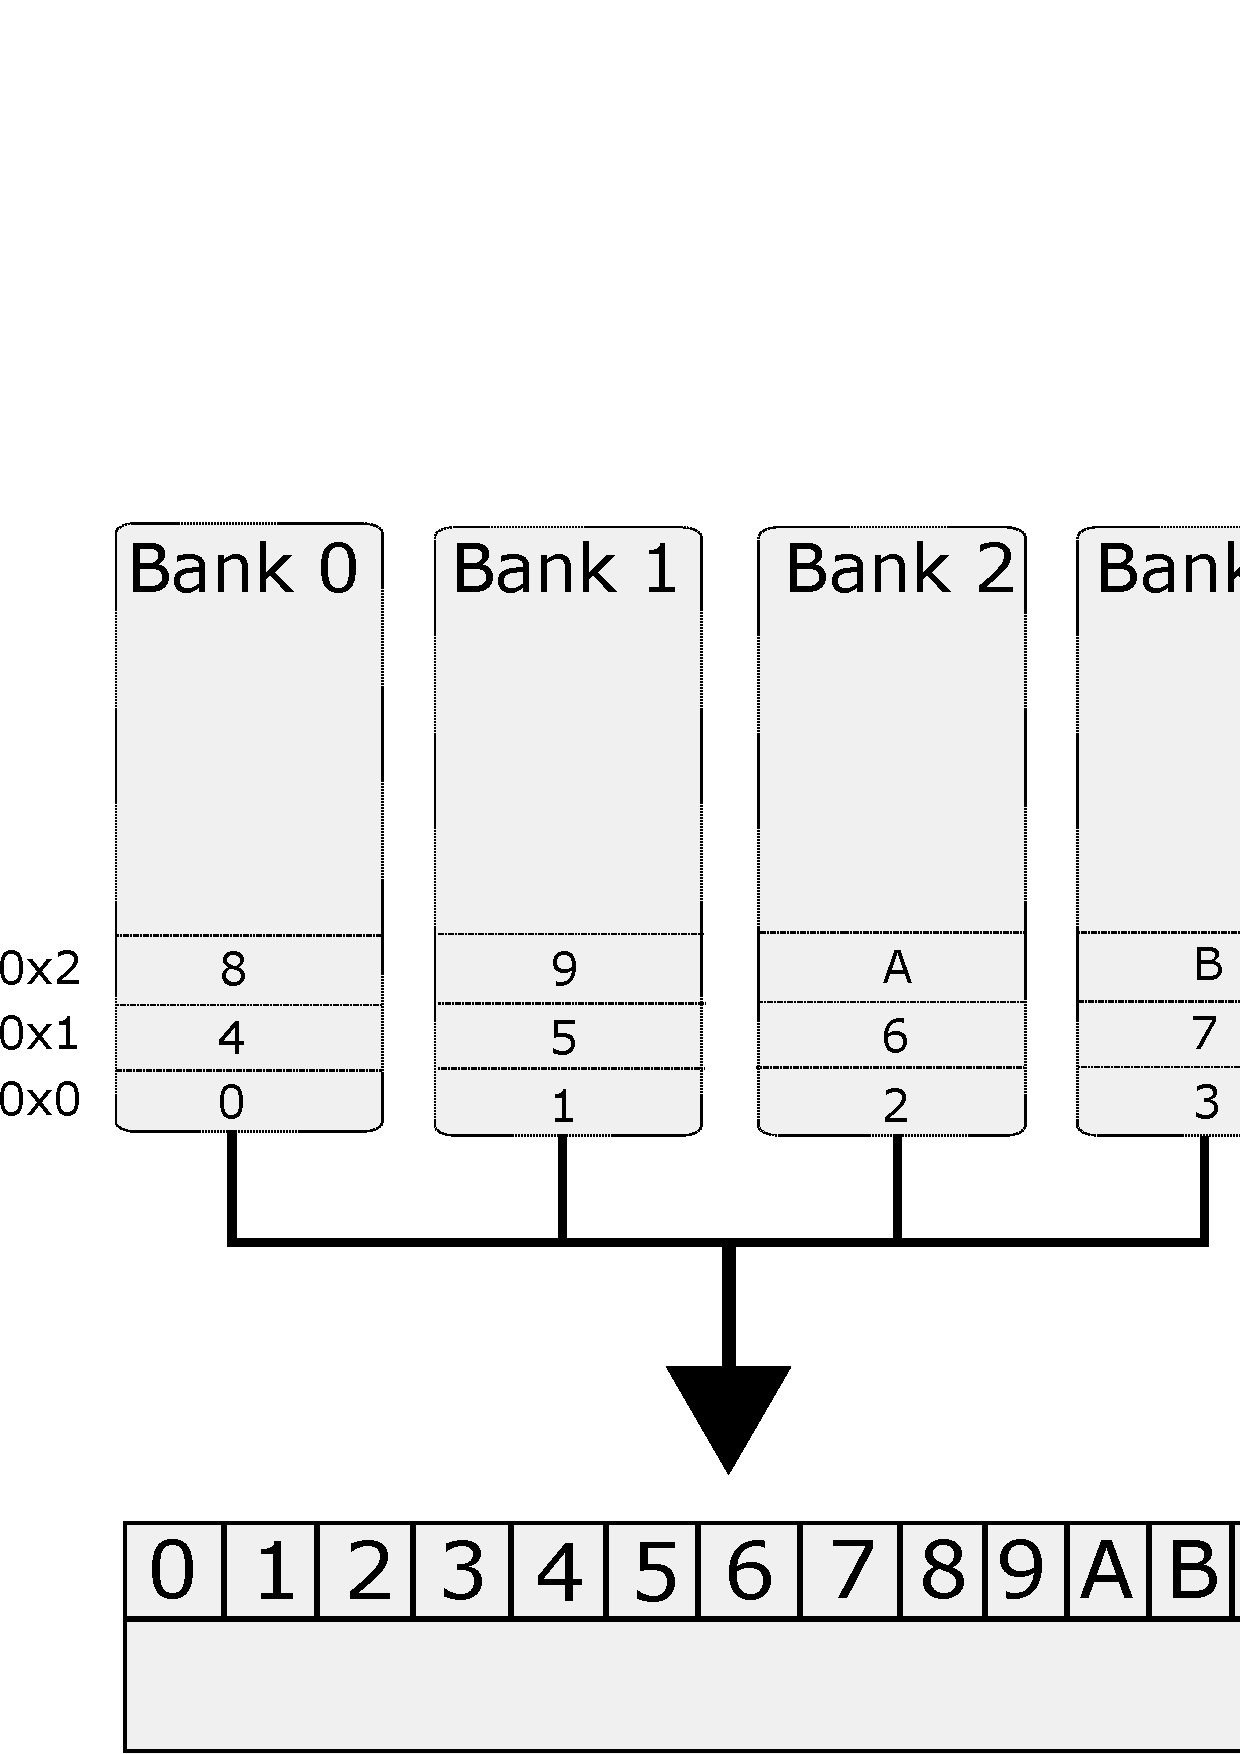
\includegraphics[width=.7\textwidth]{imgs/drawings/scalePost_explanation1.pdf}
 \end{figure}
 One pass with mask set to 1+2=3.\\
 \begin{figure}[H]
 \centering
 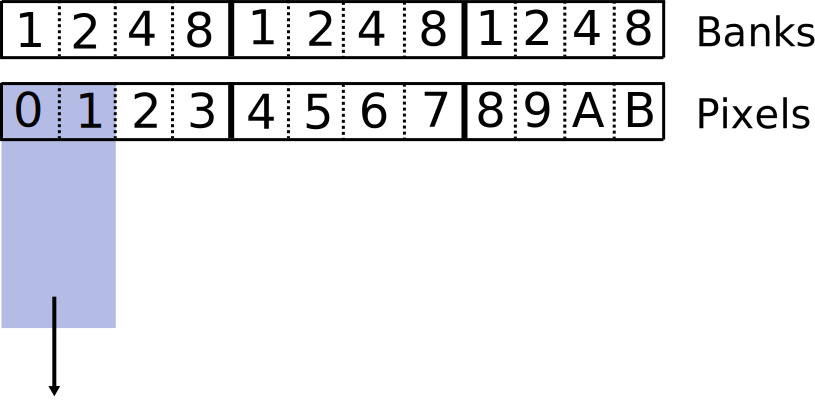
\includegraphics[width=.7\textwidth]{imgs/drawings/scalePost_explanation2.pdf}
 \end{figure}
Two passes with mask set to 8 and then 1.
  \begin{figure}[H]
 \centering
 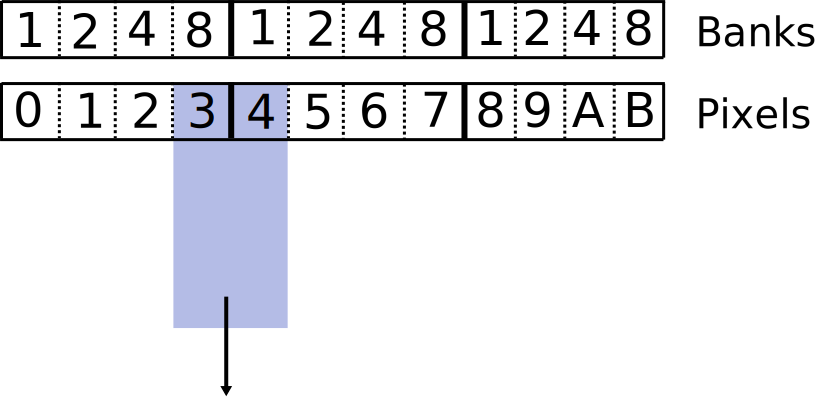
\includegraphics[width=.7\textwidth]{imgs/drawings/scalePost_explanation3.pdf}
 \end{figure}

  \begin{figure}[H]
 \centering
 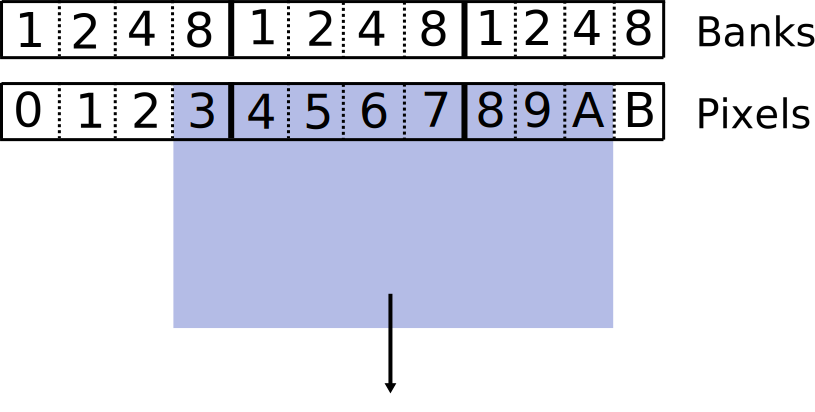
\includegraphics[width=.7\textwidth]{imgs/drawings/scalePost_explanation4.pdf}
 \caption{Thee Passes with mask set to: 8,15,14}
 \end{figure}

   \begin{figure}[H]
 \centering
 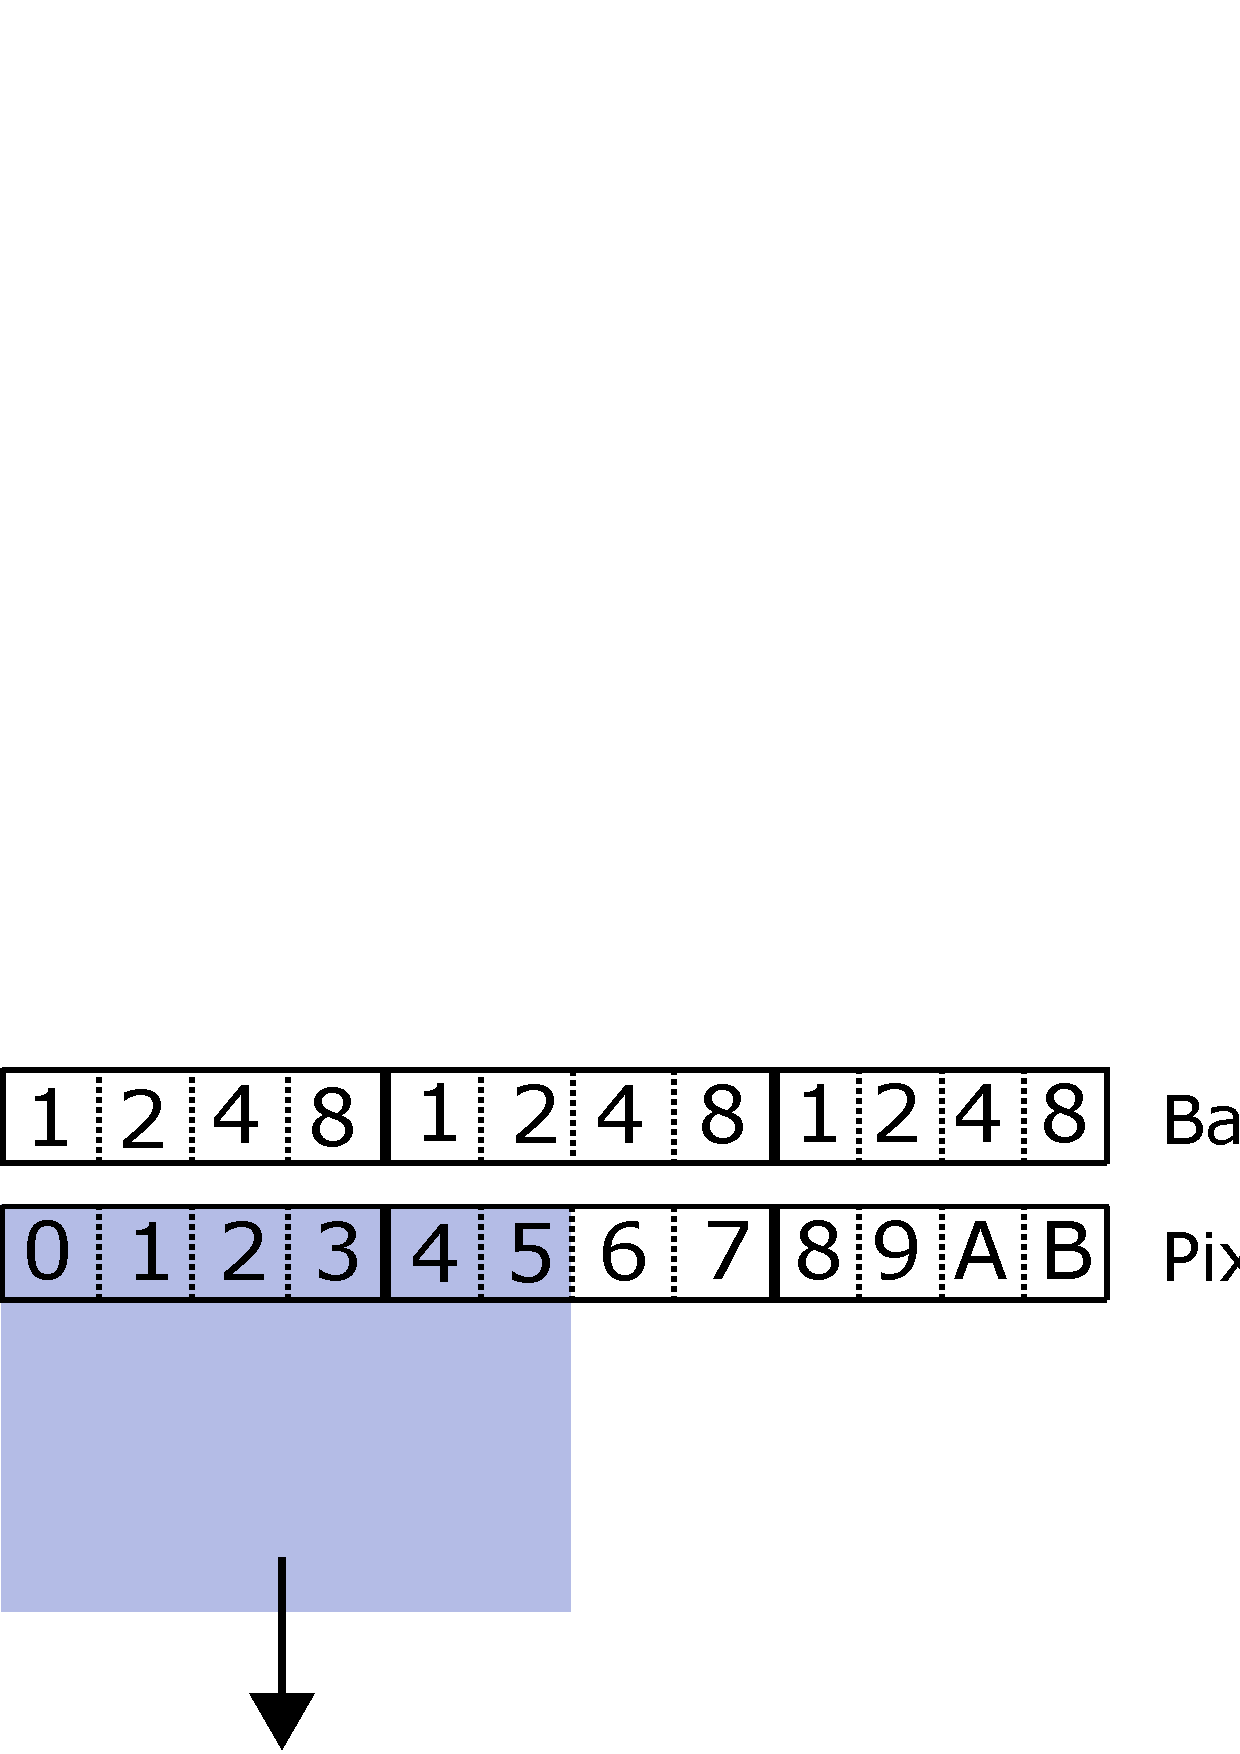
\includegraphics[width=.7\textwidth]{imgs/drawings/scalePost_explanation5.pdf}
  \caption{wo Passes with mask set to: 15 and then 3}
 \end{figure}


The instruction \codeword{or al , al} can be surprising. It means test if al is equal to zero and set the flag. Back in the day it was more populate than \codeword{test al, al}
 the VGA bank masks are harcoded in an array: One for each pass:\\
 \par
 \begin{minipage}{\textwidth}
\lstinputlisting[language=C]{code/hardcoded_masks.c}
\end{minipage}
TODO: Were images stored rotated 90 degres to increase cache hit ? No way, this was aimed at 386. BUT that would make the drawing easier !!

In the following example, the left wall is magnified. several rays hit the wall at the same texture location.
\begin{figure}[H]
 \centering
 \fullimage{post_optimization_1_show.png}
\end{figure}
The engine takes advantage of it and draw several columns (posts) efficiently with the VGA. The engine was altered to show the optimized posts in pink.
\begin{figure}[H]
 \centering
 \fullimage{post_optimization_1_pink_show.png}
\end{figure}

In the previous scene, 20\% of the wall was optimized away. In the next two screenshot, the same process, this time with the `eagle' texture:
\begin{figure}[H]
 \centering
 \fullimage{post_optimization_2_show.png}
\end{figure}


\begin{figure}[H]
 \centering
 \fullimage{post_optimization_2_pink_show.png}
\end{figure}
 
To draw several column of pixels at the same time, the engine exploit the VGA banks and the masking mechanism seen in the Hardware section.
Since up to eight column can be similar, there are many case of figure depending on the alignment with the VGA banks and how many pixels to draw:























\subsubsection{Texturing}
A subtle but extremely efficient trick used to improve rendition is pre-baked light texture. The wall textures are generated twice by the artists: Once light and once dark:\\
  \begin{figure}[H]
\centering
 \fullimage{baked_lights_wood.png}
 \end{figure}
\par
  \begin{figure}[H]
\centering
 \fullimage{baked_lights_stone.png}
 \end{figure}
\par
At runtime, upon casting each ray: if the ray hit a vertical wall the engine uses a light texture. If the ray hits an horizontal wall, it uses the dark version of the same texture. it is not obvious but when the same scene is rendered with and without and both screenshots are next to each others, the difference is vivid:\\
\begin{minipage}{\textwidth}
\begin{figure}[H]
\centering
 \fullimage{backed_off.png}
 \caption{Here: Baked texture off. Next: Backed texture on.}
 \end{figure}

\begin{figure}[H]
\centering
 \fullimage{backed_on.png}
 
 \end{figure}
 \end{minipage}




 





\subsubsection{Door}
Doors have no tickness.\\
doorposition[] holds the amount the door is open, ranging from 0 to 0xffff
  this is directly accessed by AsmRefresh during rendering\\
  // don't close on anything solid\\
\begin{figure}[H]
 \centering
 \fullimage{door_flat.png}
\end{figure}

\par
TODO: Explaih half step added.\\
\par 
 \par
\begin{figure}[H]
  \centering
 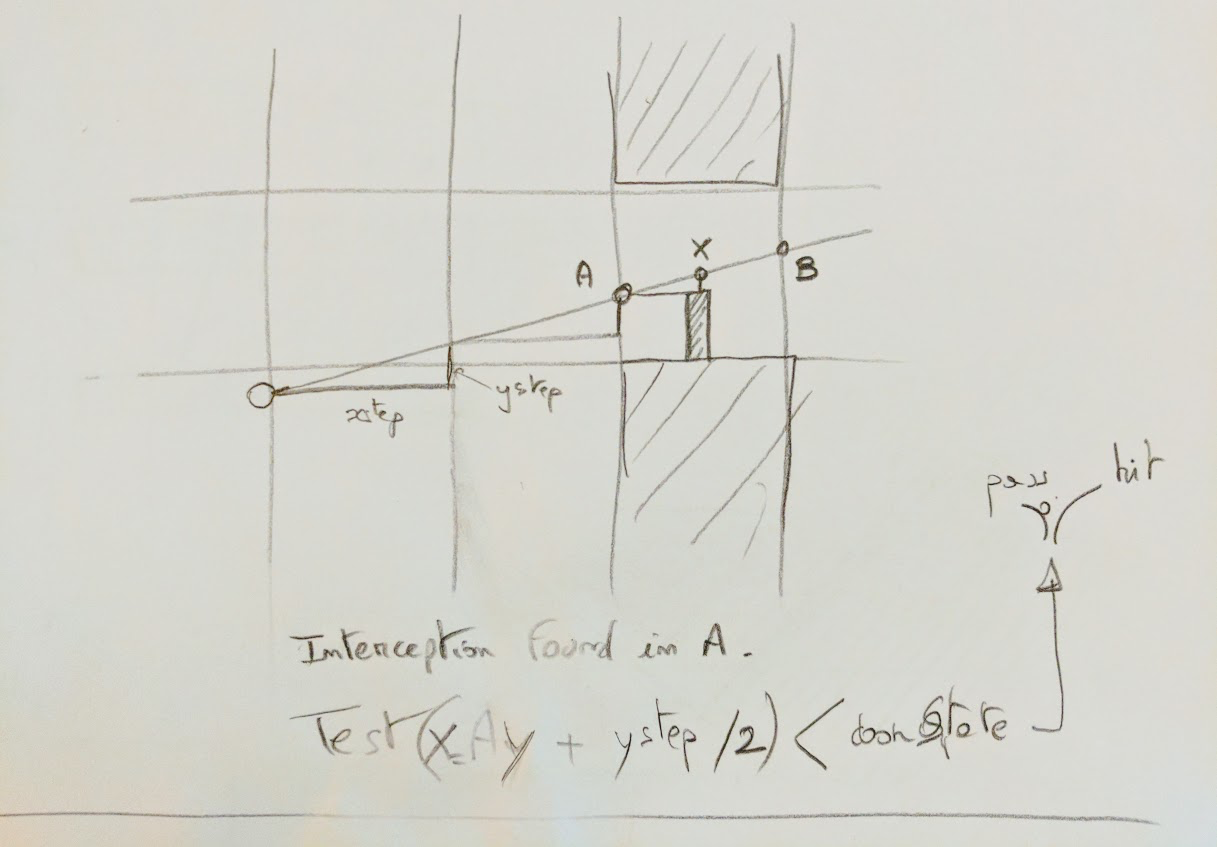
\includegraphics[width=\textwidth]{imgs/drawings/test_door.png}
\end{figure}
\par












\subsubsection{Push walls} 
Push walls are very similar to doors except they "open" away from the player instead of sideway.\\
\par
Tom had to really push to get pushwalls (hidden walls).\\


















\subsection{Drawing things}
Once the walls are drawn, it is time to render sprites such as enemies, items (ammos, weapons) and decoration (lamps, table, etc). Two goals must be reached:
 \begin{enumerate}
  \item Find which sprites are visible.
  \item Draw them correctly (parts hidden behind a wall should not be drawn)
 \end{enumerate}



\subsubsection{Visible Sprite Determination}
Building a list of visible sprite is done indirectly by leveraging raycaster information. The visible sprites are on visible tiles. So the raycaster remember all tiles it visited.\\
\begin{figure}[H]
  \centering
  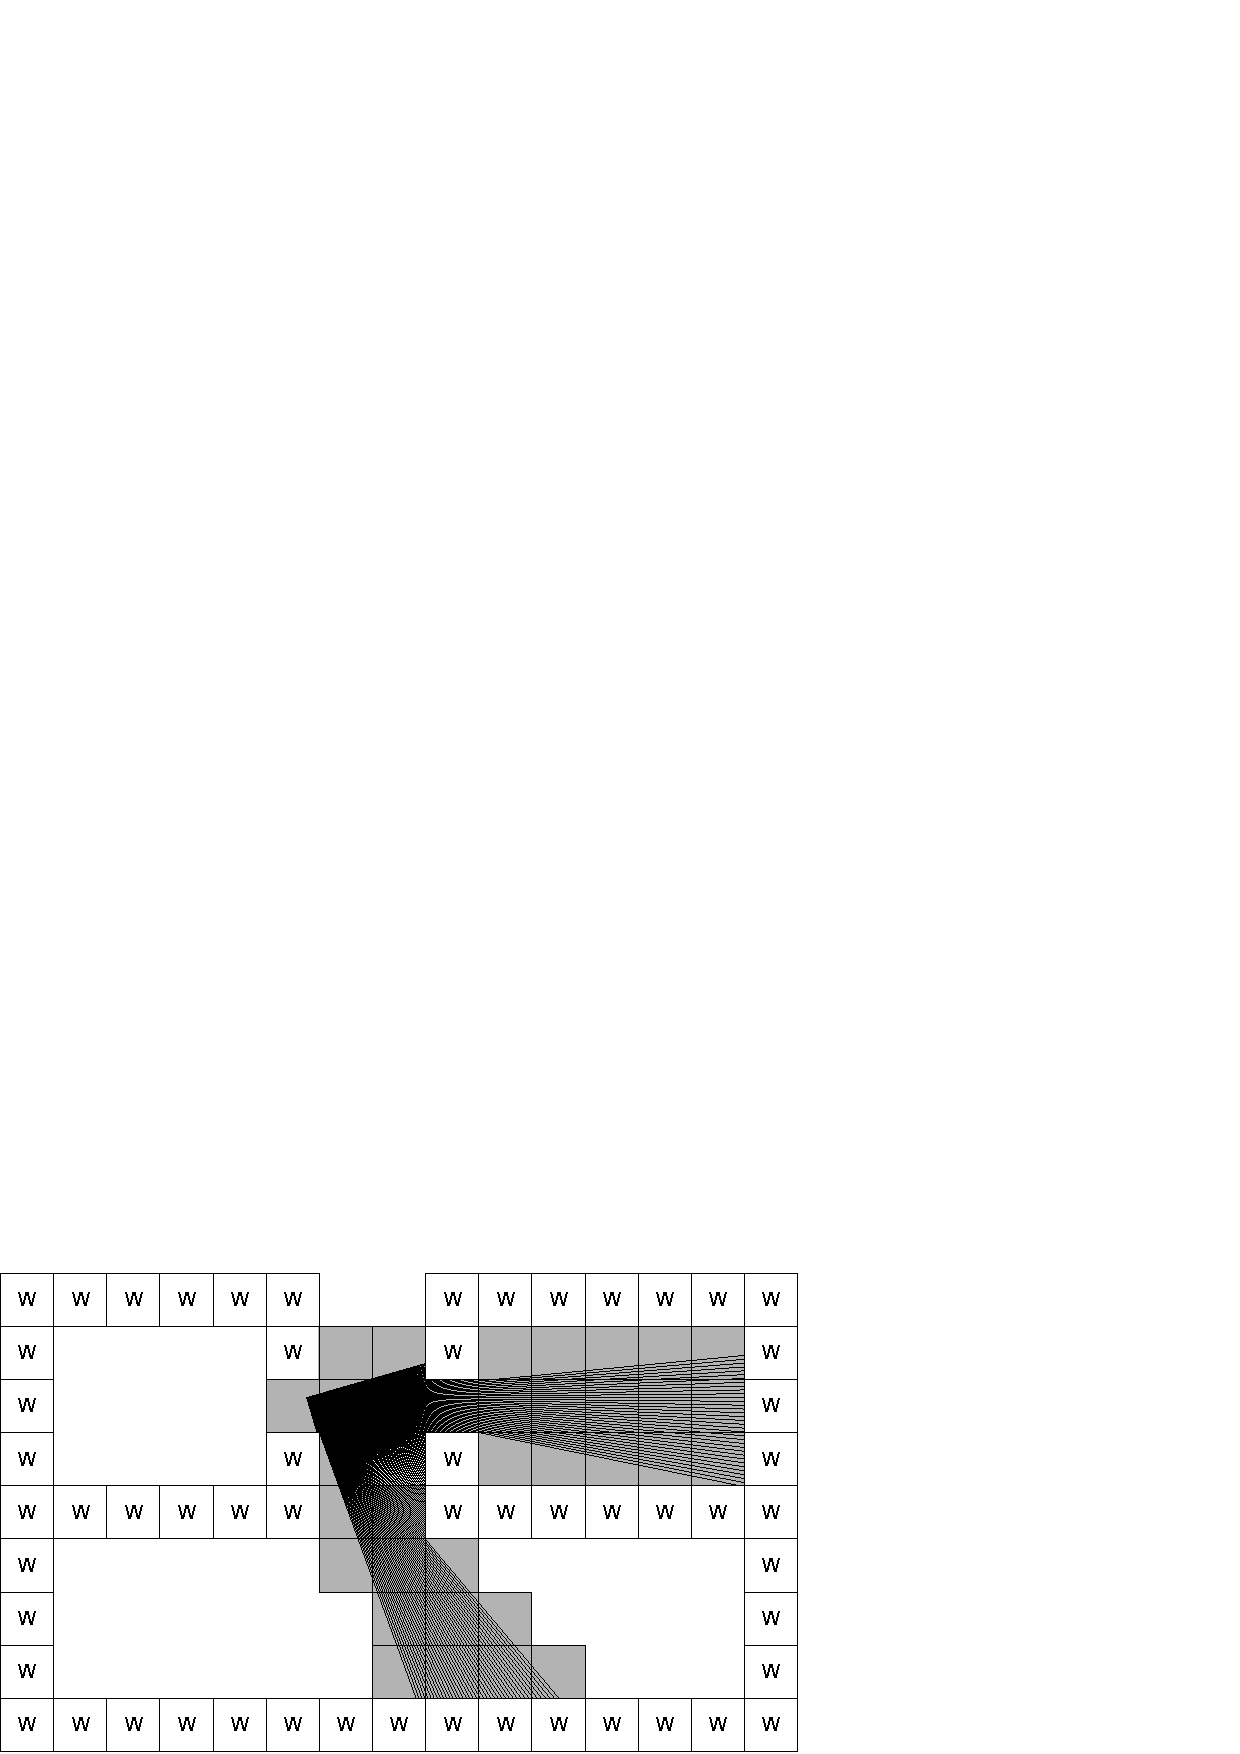
\includegraphics[width=\textwidth]{imgs/drawings/ray_caster_explained/marked_out_room.pdf}
 \caption{Ray cast and visible spots.} 
\end{figure}
This is done with a 64x64 boolean array indicating if a tile was visited during raycasting. At the beginning of each frame, the engine clears the array:
 \lstinputlisting[language=C]{code/clear_vis_wold3d.c}
 Note that because register are 2 bytes wide, an array of 64x64=4096 bytes can be zeroed in 2048 iterations. Nowadays it is more efficient to use the C library.
 \lstinputlisting[language=C]{code/clear_vis_modern.c}
 Later in the assembly hand crafted procedure \codeword{AsmRefresh}
  \lstinputlisting[language={[x86masm]Assembler}]{code/mark_vis_wold3d.asm}
  
 To build a list of visible sprites, the engine goes over the full map and for each entity, check if a ray passed by its tile coordinate. If yes, the sprite is added to the visible list.
\par
\bu{Trivia :} MAXVISABLE=50\\
\par




\subsubsection{Rendition}
With a list of visible entities, the engine news to draw them on screen correctly. Each sprites is transformed from map space to player space. 

\par
\begin{figure}[H]
\centering
 \includegraphics[width=\textwidth]{imgs/drawings/spaces.pdf}
 \end{figure}
\par
The X coordinate is used to place a sprite horizontally on the screen. They don't need to be place vertically for the good reason that all sprites and texture are drown in the same 64x64 space representing 8 feet by 8 feet. As shown in the following screenshot, scaling vertically a sprite is enough to give the illusion of perspective:\\
\par
\begin{figure}[H]
 \centering
 \fullimage{drawing_things.png}
\end{figure}

Even objects with only a part on the ground (meat) of with wide empty in between (lamp with shadow) are actually just one sprite centered and scaled vertically:\\

\par
  \begin{minipage}{.5\textwidth}
     \fullimage{guard_sprite.png}
  \end{minipage}
   \begin{minipage}{.5\textwidth} 
     \fullimage{wall_texturw.png} 
   \end{minipage}

\par

  \begin{minipage}{.5\textwidth} 
     \fullimage{sprite_food.png} 
   \end{minipage}
  \begin{minipage}{.5\textwidth} 
     \fullimage{light_sprite.png}
   \end{minipage}

\par

Trivia: The sprites with a lot of transparency (such as the food and the lamp shown previously) would later turn out a major fillrate issue with hardware accelerated renderer for the iOS port:

\begin{fancyquotes}
Wolfenstein (and Doom) originally drew the characters as sparse stretched columns of solid pixels (vertical instead of horizontal for efficiency in interleaved planar mode-X VGA), but OpenGL versions need to generate a square texture with transparent pixels.  Typically this is then drawn by either alpha blending or alpha testing a big quad that is mostly empty space.  You could play through several early levels of Wolf without this being a problem, but in later levels there are often large fields of dozens of items that stack up to enough overdraw to max out the GPU and drop the framerate to 20 fps.  The solution is to bound the solid pixels in the texture and only draw that restricted area, which solves the problem with most items, but Wolf has a few different heavily used ceiling lamp textures that have a small lamp at the top and a thin but full width shadow at the bottom.  A single bounds doesn't exclude many texels, so I wound up including two bounds, which made them render many times faster. 
\bigskip \\
\textbf{John Carmack - Programmer}
 \end{fancyquotes}

\par

The transparency of the sprite is exploited to reduce the storage and RAM consumption. They are stored in a special format skipping transparent section. The routine in charge of drawing decompress a column of sprite while it draws which mean the precomiled scaler cannot be used to draw sprite since they don't handle transparency. Instead a custom assembly crafter routine takes care of decompressing sprite and scaling them on screen.
\par
TODO: C code sample?















\subsubsection{Clipping}
There is a second benefit to have wall and sprite in the same 64x64 coordinate system: It is easy to clip. Once the actor's distance is calculated, a height can be generated. There height are the same type calculated for the walls. As a result, for each column to find out if a column if behind a wall, the engine just compare the height from the occlusion array to the height of the actor:\\
\par
Drawing things far to near is good for transparency but does not guaranty correctness. When a sprite is partially behind a wall or a door, it has to be clipped. This is done thanks to an occlusion array. While drawing the walls and doors, the engine also maintains an array in which it records the height of the column:\\
\par
\begin{minipage}{\textwidth}
\lstinputlisting[language=C]{code/wallheight_declaration.c}
\end{minipage}
\begin{minipage}{\textwidth}
\lstinputlisting[language=C]{code/wallheight_population.c}
\end{minipage}
\begin{minipage}{\textwidth}
\lstinputlisting[language=C]{code/wallheight_usage.c}
\end{minipage}
\par
Since all sprite and walls are in the same coordinate system, clipping is as easy as a height comparison:\\
















\subsection{Drawing weapon}
Drawing the weapon at the bottom is straight forward. This part of the code just uses the precompiled scalar with no clipping. Nothing much to say about that :/!\\


















\subsection{A.I}
The 3D engine not only draw things, it also allows all objects to "think" and take actions. Those thinking objects are called "actors" and help to keep the game exciting and improve immersion. If enemies are too predictable and easy to defeat the game becomes boring. The designer and programmers worked in tandem on this one: The engine maintains a state machine for each thinker but it also relies heavily on hints and clues on the map provided by the designers to make enemies appear smarter than they are.\\
\par







"Actors" can be aggressive, they can be sneaky or they can be dumb (like when they are a rockets). To mode the behavior, all enemies have an associated state:
\begin{itemize}
\item Standing
\item Attack
\item Path
\item Pain
\item Shoot
\item Chase
\item Die
\item Special Boss state
\end{itemize}

With each state are associated think and action method pointer. There is also a \cw{next} to indicate which state the actor should transition to once it is finished with the current state/action:\\
\par
\begin{minipage}{\textwidth}
\lstinputlisting[language=C]{code/statetype.c}
\end{minipage}
\par


A guard in standing position always stays in the same state (\cw{next} points to itself):\\
\par

\begin{minipage}{\textwidth}
\lstinputlisting[language=C,style=mystyle,basicstyle=\small,morekeywords={statetype, NULL, true, false}]{code/s_grdstand.c}
\end{minipage}
\par
Some state chain are more complex like for example chasing:\\

\par
\begin{minipage}{\textwidth}
\lstinputlisting[language=C,style=mystyle,basicstyle=\small]{code/s_grdchase.c}
\end{minipage}
\par
This example was just for guards. All different types of enemies including bosses have their own state machine. They often share action (e.g: \cw{T\_Stand} and \cw{T\_Path} but they also occassionally have their own).\\

\par
What makes enemies interesting to interact with is how the go from standing to being aggressive via \cw{T\_Stand}. They have three ways to detect the player:\\
\begin{itemize}
\item Proximity
\item Sight
\item Noise
\end{itemize}
By far the sound is the most important and what makes the player feel like the A.I is smart. Sound propagation has always been well done in id Software engines despite receiving little coverage.





\subsubsection{Sound propagation reaction}
Early one the game teaches the player that enemies will react to gunfire and seek where the sound was coming from. Sound is an essential part of the experience. The engine takes care of it in a simple and resource efficient way: Maps are preprocessed, with each room defining an area. At runtime, the engine keeps track of what door opens and what door closes and maintains a matrix of portal connecting areas.
Knowing if an enemy can hear the main character gunfire is a simple lookup in a table.

\par
\begin{figure}[H]
 \centering
 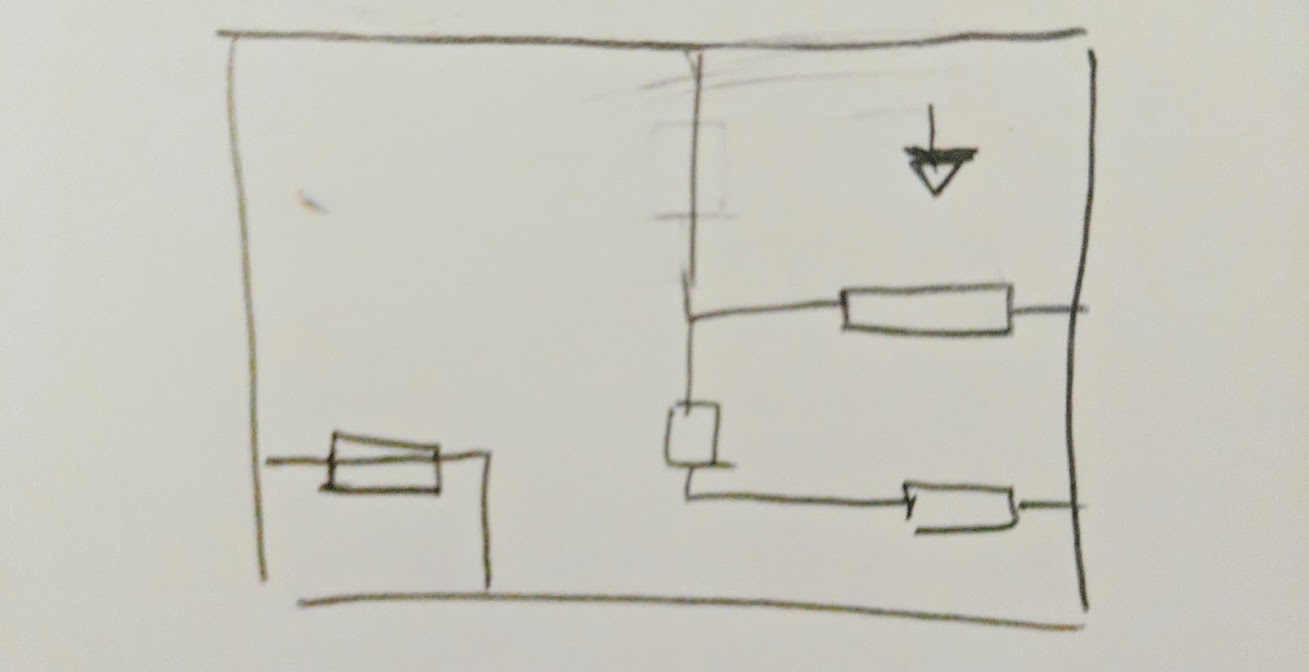
\includegraphics[width=.75\textwidth]{imgs/drawings/sound_area/map.pdf}
\end{figure}
\par

\par
\begin{figure}[H]
 \centering
 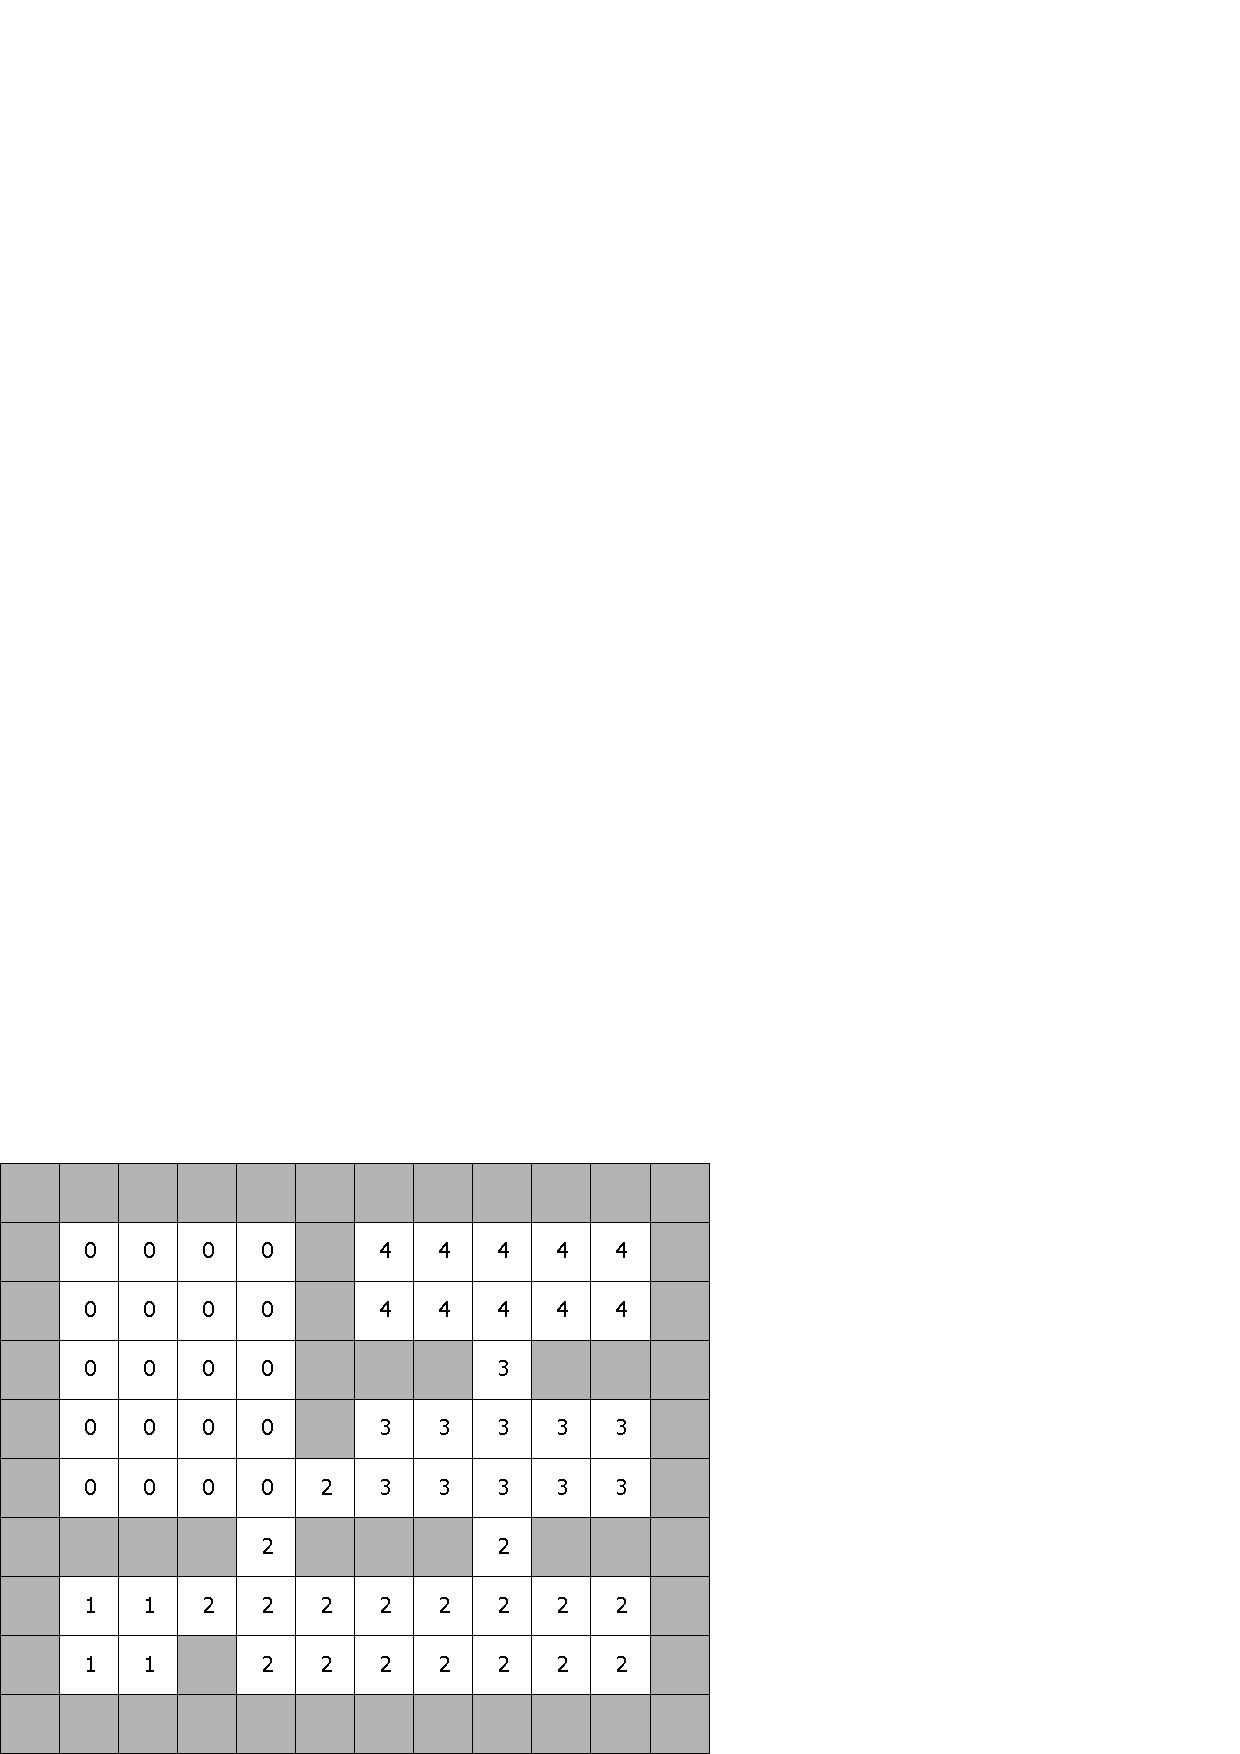
\includegraphics[width=.75\textwidth]{imgs/drawings/sound_area/area.pdf}
\end{figure}
\par
% $
% \begin{bmatrix} 1 & 2 & 3 \\ 4 & 5 & 6 \end{bmatrix}
% $
\par
\begin{figure}[H]
 \centering
 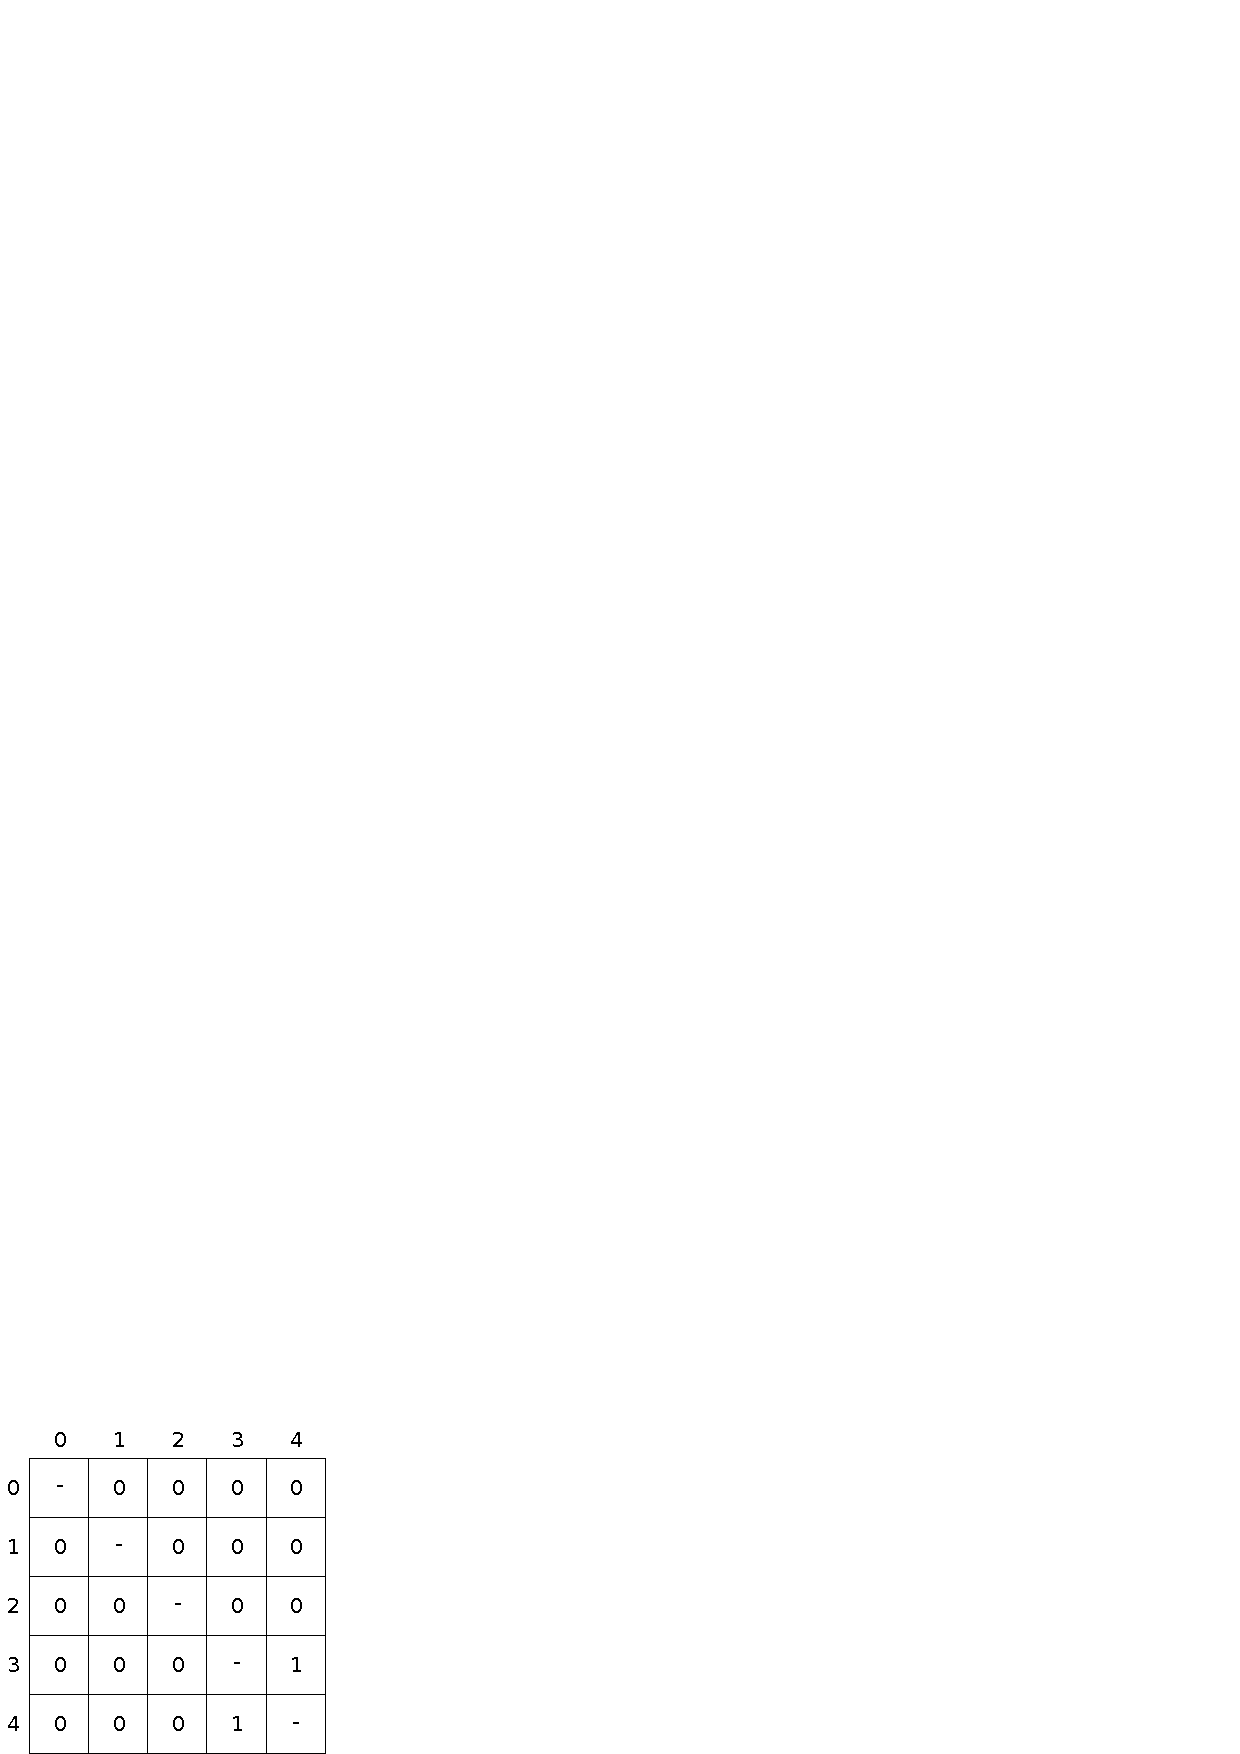
\includegraphics[width=.5\textwidth]{imgs/drawings/soud_propagation/areaconnect.pdf}
\end{figure}
\par

\par
\begin{figure}[H]
 \centering
 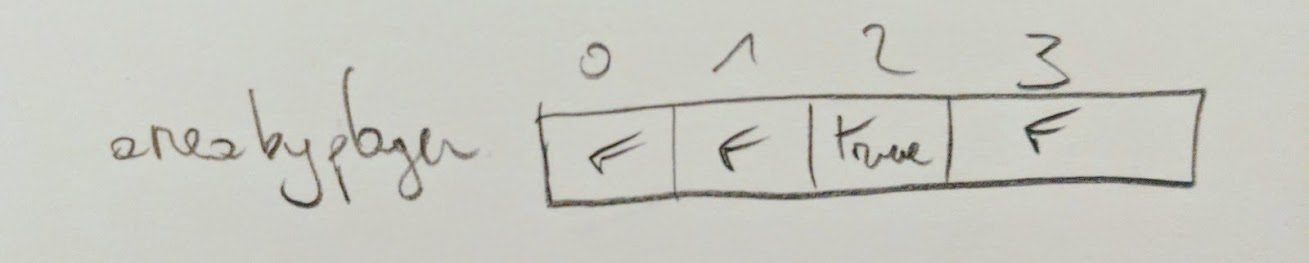
\includegraphics[width=.5\textwidth]{imgs/drawings/soud_propagation/areabyplayer.pdf}
\end{figure}
\par
37 long. Empirical value?








However this is a simple model. When a gun is fired, all enemies which could hear it will shout "Achtung!" (Attention!") and converge toward the origin of the sound. That would get old pretty fast. So the designers introduced a little hack that goes a long way.

\par
\begin{figure}[H]
 \centering
 \fullimage{ambush/map_unknown.png}
\end{figure}
\par

\begin{minipage}{0.6\textwidth}
Some tiles in the map can be marked as "AMBUSH" tile. If a guard is standing on it, he will NOT react to sounds. He is deaf. Or smart if you prefer. This is introduced early on in E1M1, the character just neutralized an enemy in a corridor. At this point it has never encountered an ambush so the player assumes the area is clear:\\
\end{minipage}
\begin{minipage}{0.4\textwidth}
\begin{flushright}
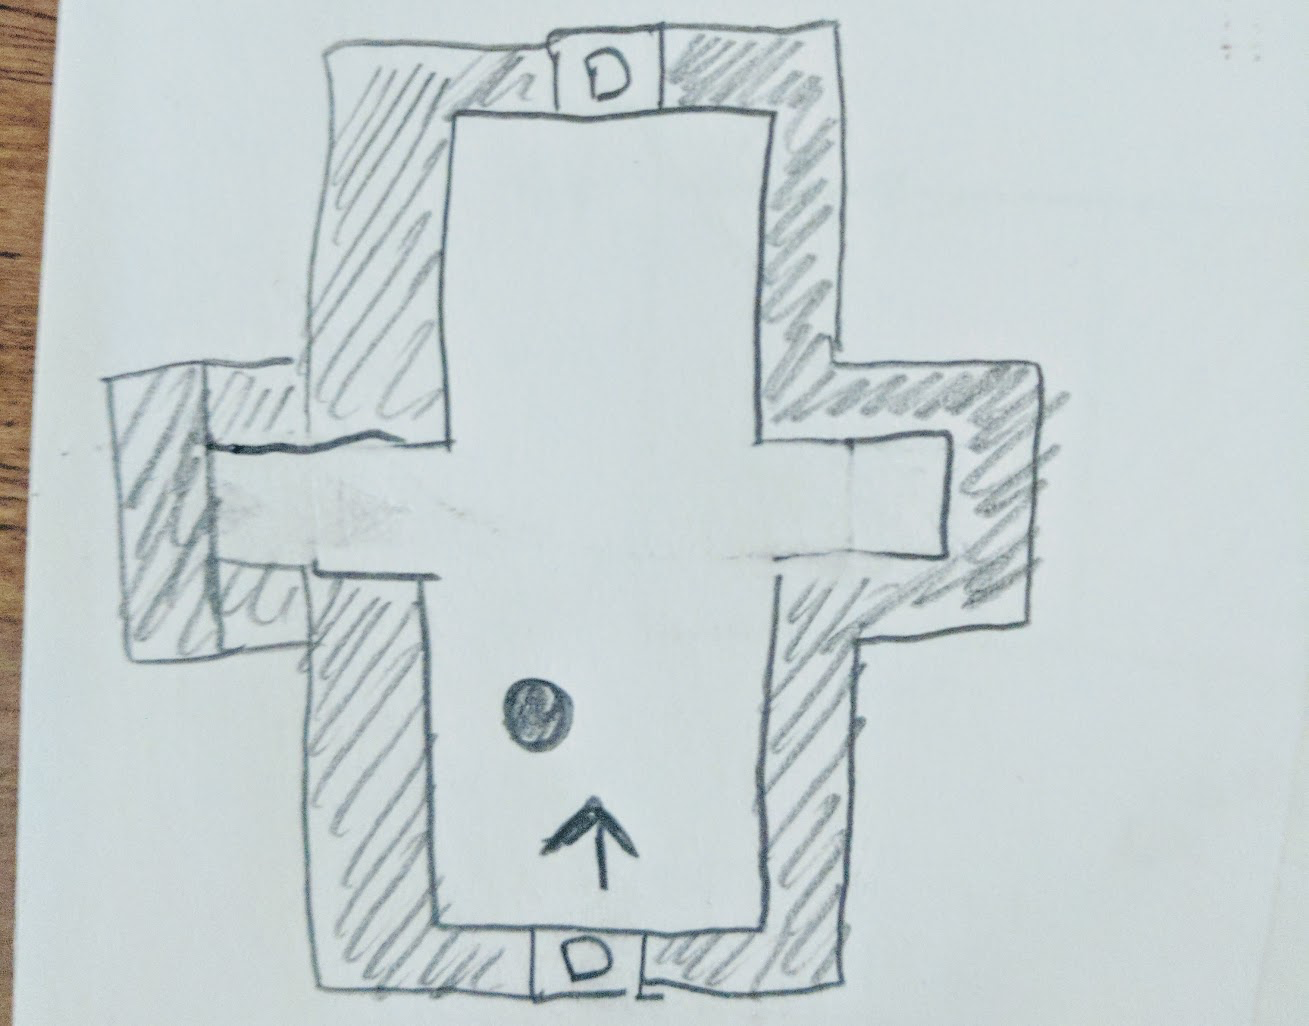
\includegraphics[width=0.98\textwidth]{imgs/drawings/ambush/map_unknown_drawing.pdf}
\end{flushright}  
\end{minipage}
\noindent
\\


\par
\begin{figure}[H]
 \centering
 \fullimage{ambush/map_ambushed.png}
\end{figure}
\par
\begin{minipage}{0.6\textwidth}
So the player will relax and either go straight to the door or maybe go left (or worse: right) to see what is in these corners. And bam: AMBUSH.
\end{minipage}
\begin{minipage}{0.4\textwidth}
\begin{flushright}
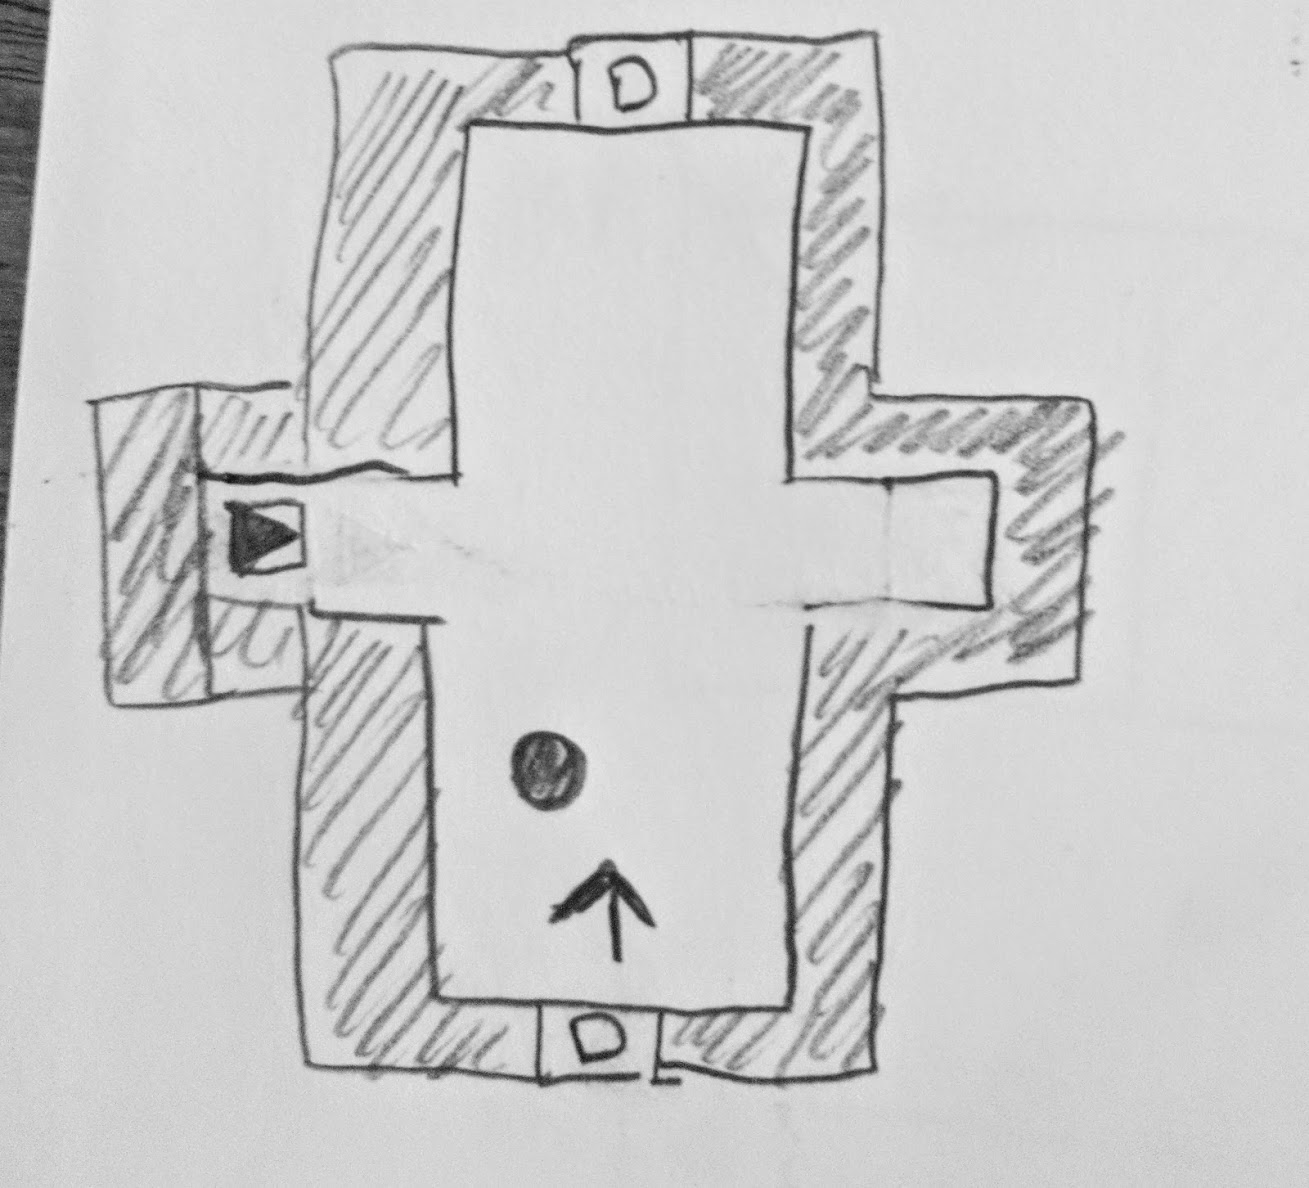
\includegraphics[width=0.98\textwidth]{imgs/drawings/ambush/map_ambushed_drawing.pdf}
\end{flushright}
\end{minipage}
\noindent
\\

This is probably one of the cheapest feature in the engine which yet resulted in what most would agree is the soul of the game: Immersion.\\
\par

\bu{Trivia :} The ambush behavior is explained in the Hint Book as follow:\\
\par
\begin{fancyquotes}
Each enemy is given specific orders which dictate his actions once he knows of your presence. Some are ordered to immediately attack, while others are trained to act only upon visual contact.
 \bigskip \\
\bigskip \\
\textbf{Kevin Cloud. The Official Hint Manual for Wolfenstein 3D}
 \end{fancyquotes}

\bu{Trivia :} Bug or dedication to ambush, a guard on a n AMBUSH tile will react ONLY to the player sight. Seeing an other actor die in front of him will not activate him.\\


\subsubsection{Patrolling}
I/A also faked with map waypoint for patrolling.\\
\par
\par
\begin{figure}[H]
 \centering
 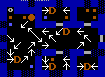
\includegraphics[width=0.98\textwidth]{imgs/drawings/path.png}
\end{figure}
\par

% \subsubsection{Vision reaction}
% \subsubsection{Proximity reaction}
% \subsection{Pursuit and opening doors}
% \subsubsection{Firing at player}






